%%%%%%%%%%% seconda parte del corso - MobiDEV %%%%%%%%%%% 
\chapter{Posizionamento indoor - MobiDEV}
\lhead{Posizionamento indoor - MobiDEV}
\rhead{Lezione 1 - 1 marzo}
\begin{center}
    \textbf{--------- Lezione 1 - 1 marzo 2021 ---------}
\end{center}

\section{Concetti preliminari}
\subsection{Calcolo della posizione indoor vs outdoor}
La maggior parte delle app richiede una maggior precisione, l'altezza infatti è fondamentale: sono al primo o al quinto piano di un edificio?
Negli ambienti outdoor l'altezza non è così fondamentale.

Le tecniche che utilizziamo in outdoor non possono essere utilizzate in indoor:
\begin{itemize}
    \item GPS: linea di comunicazione tra la sorgente (satellite) e il dispositivo
    \item le interferenze possono rendere inutilizzabile il sistema segnale, come il segnale radio che viene disturbato da muri o da altri ostacoli
\end{itemize}  

L'area di copertura in indoor è ridotta. 
Nel maggior parte dei casi lo spostamento avviene a piedi ed il vantaggio spostandosi lentamente è che si ha una minore rapidità di spostamento degli utenti, lo svantaggio è che siamo soggetti a rumori come a cambiamenti di direzione improvvisi. 

Attualmente l'indoor positioning è ancor poco comune.

\textit{\textbf{Chi è il soggetto da localizzare?}}
\\ Possiamo voler monitorare la posizione di persone, robot o oggetti come ad esempio il carrello delle emergenze in un ospedale. 
\\ Soggetti diversi implicano tecnologie diverse:
\begin{itemize}
    \item per le persone abbiamo tecniche di posizionamento che sfruttano i dispositivi mobili degli utenti
    \item per i robot e gli oggetti possiamo prevedere un hardware apposito
\end{itemize}

\textit{\textbf{Chi effettua il calcolo della posizione?}} 
\\ Ci sono due tipi di tecniche: 
\begin{itemize}
    \item tecniche attive: il calcolo della posizione viene effettuato dal dispositivo in movimento (le tecniche trattate nel corso)
    \item tecniche passive: l'hardware distribuito nell'ambiente capisce in che posizione sono gli utenti 
\end{itemize}

\subsection{Applicazioni principali}
\begin{itemize}
    \item navigazione: non è una tecnologia molto utilizzata. Sapere dove muovermi all'interno di un aeroporto sarebbe comodo, come ad esempio "guidami fino al gate 15"
    \item location based services: vengono utilizzati per l'outdoor, non ancora per l'indoor 
    \item home automation: es. un sistema che in base alla stanza nel quale mi sposto, accende le luci
    \item context detection: es. il riconoscimento precoce di malattie degenerative tramite un'analisi del comportamento degli utenti
    \item social networking: es. friend finder
    \item emergenze: es. in caso di incendio i vigili del fuoco sanno dove sono le persone da salvare
\end{itemize}

\subsection{Paradigmi di navigazione}
\begin{itemize}
    \item Navigazione allocentrica: il sistema fornisce le indicazioni di navigazione rispetto all'ambiente come ad esempio la vista dall'alto con la mappa. 
    \item Navigazione egocentrica: il sistema fornisce le indicazioni di navigazione rispetto all'utente, come ad esempio una freccia che indica dove andare
\end{itemize}
L'interpretazione da parte dell'utente delle informazioni allocentriche richiede all'utente di conoscere com'è orientato e non sempre questa navigazione è possibile quando c'è ad esempio del fumo o della nebbia. 

\subsection{Caratteristiche dei sistemi di posizionamento indoor}
Quali caratteristiche deve avere il sistema per adattarsi alle necessità dell'utente?
\begin{itemize}
    \item il sistema indoor deve essere preciso nel calcolo della posizione
    \item area di copertura (stanza, edificio, globale)
    \item il costo (di installazione, di manutenzione, ecc.)
    \item infrastruttura (nessuna, trasmettitori sparsi nell'ambiente, ecc.)
    \item maturità della tecnologia (prototipo, prodotto, ecc.)
    \item tipo di informazione di posizione che viene prodotto (posizione 2D/3D, orientamento, ecc)
    \item privacy (il sistema viene a sapere dove si trova l'utente?)
    \item frequenza di update (quando l'utente fa qualcosa, automatico ogni 4 secondi)
    \item azione richiesta all’utente (nessuna, inquadrare il marker, ecc.)
    \item interfaccia (grafica, vocale, ecc.)
    \item robustezza della misura (nelle giornate affollate, ecc.)
    \item robustezza della sistema (i beacon si possono rubare, i marcatori si staccano, ecc.)
    \item scalabilità (non scalabile, scalabile aumentando l’infrastruttura, scalabile diminuendo l’accuratezza, ecc.)
    \item impatto sull'ambiente (i marcatori visivi rovinano l’aspetto estetico, ecc.)
\end{itemize}

\section{Tecniche di posizionamento}
Ci sono 4 tecniche di posizionamento indoor che verranno approfondite:
\begin{itemize}
    \item immagini
    \item segnali radio
    \item sistemi inerziali
    \item soluzioni ibride
\end{itemize}

\section{Tecniche basate su immagini}
Ci sono diverse tecniche che permettono di calcolare la posizione usando le immagini tra cui i marcatori visivi.
I marcatori visivi sono oggetti facilmente riconoscibili tramite tecniche di computer vision. Distinguiamo marcatori:
\begin{itemize}
    \item espliciti: progettati per essere facilmente riconoscibili come i QR-code
    \item impliciti: creati per altri scopi, ma facilmente riconoscibili con tecniche di computer vision come i cartelli stradali
\end{itemize}

I marcatori visivi possono essere installati nell'ambiente. Quando un utente ad esempio inquadra il marcatore, so che l'utente si trova lì vicino. Ciascun marcatore contiene la propria posizione oppure un identificatore che il device sa associare alla posizione. 

\subsection{Pro e contro dei marcatori espliciti}
\begin{table}[!ht]
    \centering
    \begin{tabular}{p{.45\textwidth}|p{.45\textwidth}}
        \textbf{Vantaggi} & \textbf{Svantaggi} \\
        \hline
        \begin{itemize}
            \item tecnologia semplice e stabile 
            \item i marcatori sono economici
        \end{itemize} & 
        \begin{itemize}
            \item la precisione è legata alla distanza alla quale il device riesce a riconoscere il marcatore
            \item non permettono di calcolare l'angolo
            \item è richiesta un'azione esplicita all'utente
        \end{itemize}
    \end{tabular}
\end{table}

\subsection{I marcatori impliciti}
Se so la dimensione in centimetri del marcatore, dove viene appeso e con che angolo, quando il marcatore viene inquadrato, posso usare tecniche di geometria per capire dove si trova l'utente rispetto al marcatore. 

Però ho un problema: ho il sistema dove ho cartelli facilmente riconoscibili e sviluppo una tecnica che riconosca i cartelli ma ci potrebbero essere due cartelli uguali. 
Bisogna combinare la tecnica con altre tecniche ad esempio usando i segnali radio. 
La tecnica funziona da sola nel caso in cui i marcatori impliciti siano tutti diversi. 

\subsubsection{Pro e contro}
\begin{table}[!ht]
    \centering
    \begin{tabular}{p{.45\textwidth}|p{.45\textwidth}}
        \textbf{Vantaggi} & \textbf{Svantaggi} \\
        \hline
        Non devo installare altri segnali nell'ambiente (in alcuni ambienti potrebbe essere impossibile, ad esempio nei musei) & se i marcatori non sono univoci la tecnica da sola non permette di calcolare la posizione e deve essere combinata con altre tecniche
    \end{tabular}
\end{table}

\subsubsection{Tecniche marker-less}
Per risolvere i problemi posso usare tecniche marker-less, non vengono scelti marcatori da me programmatore ma il sistema estrae da solo delle informazioni visive che permettono poi all'utente di capire dove si trova.
Questa tecnica opera a due fasi:
\begin{itemize}
    \item setup: viene costruita una mappa 3D dell'ambiente, il sistema identifica diversi punti di riferimento con caratteristiche geometriche peculiari
    \item calcolo posizione: quando l'utente è nell'ambiente, vengono identificati alcuni punti di riferimento e poi vengono confrontati con quelli ottenuti in fase di setup, per risalire alla posizione
\end{itemize}

Ho però un problema: durante la fase di setup ho un dispositivo che mentre si muove, deve creare una mappa dell'ambiente e deve sapere dove sono rispetto all'ambiente. 

Durante la fasi di calcolo della posizione, dal device mobile si cerca di trovare gli stessi punti di riferimento identificati in fase di setup e di stimare la posizione della camera rispetto ad essi. 

Ho un problema: due zone possono avere le stesse caratteristiche, ad esempio possono esserci due stanze che presentano le stesse feature su piani diversi di un edificio.



\rhead{Lezione 2 - 4 marzo}
\begin{center}
    \textbf{--------- Lezione 2 - 4 marzo 2021 ---------}
\end{center}
\subsection{Uso di tecniche di visione per posizione outdoor}
Dalle immagini catturate dalla macchina google (street view) possiamo estrarre dei punti di riferimento (feature points). 
La posizione da cui sono scattate le foto stradali è nota con buona precisione, quindi si riesce a conoscere la posizione dei feature points.
\\ Quando l'utente inquadra attorno a sé, si conosce più o meno la posizione, e dalle immagini dell'utente si identificato le feature che corrispondono a quelle identificate dalle immagini stradali. Poi si fa un match con i feature points della macchina google in modo tale che si possa calcolare la posizione dell'utente rispetto alla macchina (dato che so come si trova la macchina rispetto ai feature points).
Si calcola la posizione (molto precisa) e l'orientamente dell'utente. 

Una funzione simile è messa a disposizione per le librerie AR da Apple (ARKit).    

\section{Calcolo della posizione basato su segnale radio}
I dispositivi mobili al momento sono dotati di hardware per questi segnali radio:
\begin{itemize}
    \item WiFi: abbiamo un problema applicativo, con le tecnologie attuali non è possibile da programma accedere alle antenne WiFi nelle vicinanze, il SO operativo conosce le informazioni ma le API dei dispositivi iOS non consentono al programmatore di accedere. 
    \item bluetooth: dispositivi detti beacon da acquistare ed installare specificamente per il calcolo della posizione
    \item Near Field Communication (NFC)
    \item Ultra Wide-Band (UWB): ancora poco diffuso nei dispositivi mobili
\end{itemize}
RSSI indica la potenza del segnale ricevuto dal dispositivo mobile. 

Ci sono 3 diverse tecniche basate su segnale radio:
\begin{itemize}
    \item prossimità
    \item multilaterazione
    \item fingerprinting
\end{itemize}

\subsection{Posizionamento per prossimità}
Il dispositivo mobile percepisce il segnale radio inviato da un'antenna con un certo identificativo. 
Se conosciamo l'id dell'antenna e la distanza massima con la quale si può percepire il segnale da quell'antenna, allora riusciamo a scoprire la posizione di un device. 

L'accuratezza con Wifi e bluetooth è bassa mentre con NFC è alta ma il calcolo della posizione avviene solo quando l'utente avvicina il device ad un sensore NFC installato nell'ambiente.

Ci sono due limiti parlando di prossimità:
\begin{itemize}
    \item si considera una sola antenna
    \item si considera solo il fatto di percepire il segnale di quell'antenna, non si prova a stimare la distanza dall'antenna stessa
\end{itemize} 

\subsection{Multilaterazione}
Posso sapere che sono vicino ad un'antenna senza sapere la distanza oppure posso provare a stimare la distanza usando RSSI ma mi aspetto che la potenza decresca con l'aumentare della distanza.

\subsubsection{Calcolo della distanza con RSSI}
Conosciamo la potenza del segnale inviato, le caratteristiche dell'antenna, vogliamo calcolare la distanza ma abbiamo un altro fattore da prendere in considerazione che non conosciamo, il path lost factor che dipende dall'ambiente (è un fattore di attenuazione del segnale). 
\\ In ambienti aperti assume un valore di 2, in ambienti indoor tra 4 e 6 e in particolari indoor ha un valore minore di 2. 
\\ Stimando con RSSI si ottengono errori troppo grandi.
\\ Una tecnica per risolvere il problema è utilizzare un WiFi Round Trip Time.
\\ Google ha proposto una soluzione basata su RTT. 
RTT è la misura che rappresenta quanto ci mette un segnale ad andare e tornare da un'antenna. 

\subsection{Fingerprinting (o "scene analysis")}
La soluzione più adottata per risolvere i problema della multilaterazione è quella del fingerprinting.
Il valore di un RSSI in un punto è più o meno sempre quello, ma se metto più antenne, è difficile che la combinazione di questi valori si ripeta in un altro punto.

Data una posizione, il fingerprint è l’insieme di coppie $<$ID, RSSI\_ID$>$ dove ID è l’identificatore di un’antenna e RSSI\_ID il suo valore di RSSI misurato nella data posizione.

Un addetto si sposta all'interno dell'edificio segnalando al sistema la posizione corrente (es: toccando con il dito sulla mappa) e poi misura la potenza del segnale.
Questa operazione viene ripetuta in tutto l'ambiente, ad esempio ogni metro e prende le misure per tutte le antenne del fingerprint. 
\\ Il risultato prende il nome di radio map. 

La radio map contiene un insieme di coppie \textbf{$<$posizione, fingerprint$>$}, quindi \textbf{$<$posizione, [$<$ID, RSSI\_ID$>$]$>$}.

Quando un utente si trova nell'ambiente e vuole calcolare la posizione, possiamo prendere il fingerprint nella posizione corrente. 

Il modo più semplice per trovare la posizione dell'utente è: 
\begin{itemize}
    \item considerare tutti fingerprint in tutte le posizioni della radio-map
    \item calcolare il fingerprint dell'utente
    \item calcolare la distanza dal fingerprint in radio map
    \item vedere a quale campione l'utente è più vicino e assumo che quel campione sia la sua posizione
\end{itemize}


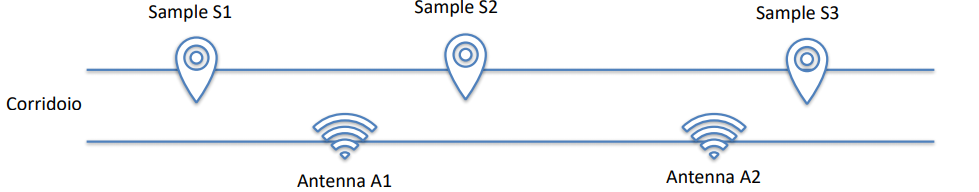
\includegraphics[width = \textwidth]{images/MobiDEV/1. posizionamento indoor/fingerprinting 1.PNG}

Ad esempio ho un corridoio con due antenne e riesco a percepirne sempre il segnale. Un incaricato misura i fingerprint in 3 posizioni campione e misura su ognuna la potenza del segnale. 
La radio map è l'insieme composto dai seguenti elementi: 
\begin{itemize}
    \item $<$S1, [$<$A1, 0,5$>$, $<$A2, 0,01$>$]$>$
    \item $<$S2, [$<$A1, 0,4$>$, $<$A2, 0,6$>$]$>$
    \item $<$S3, [$<$A1, 0,1$>$, $<$A2, 0,8$>$]$>$
\end{itemize}

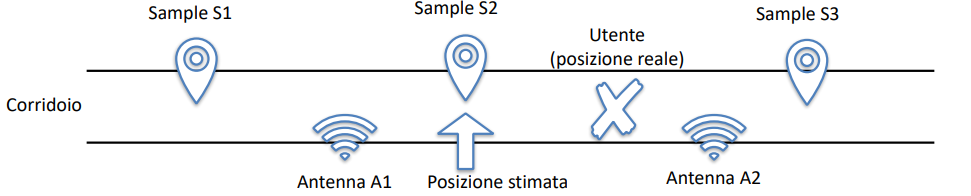
\includegraphics[width = \textwidth]{images/MobiDEV/1. posizionamento indoor/fingerprinting 2.PNG}

Il fingerprint calcolato dell'utente è [$<$A1, 0,3$>$, $<$A2, 0,7$>$].
Si procede con il calcolo delle distanze da fingerprint in radio map:
\begin{itemize}
    \item S1: $|$0,3-0,5$|$ + $|$0,7-0,01$|$ = 0,2 + 0,699 = 0,899
    \item S2: $|$0,3-0,4$|$ + $|$0,7-0,6$|$ = 0,1 + 0,1 = 0,2
    \item S3: $|$0,3-0,1$|$ + $|$0,7-0,8$|$ = 0,2 + 0,1 = 0,3
\end{itemize}
La distanza è minore rispetto ad S2 e quindi assumo che la posizione dell'utente sia quella di S2. 

Se tutto va bene trovo effettivamente il fingerprint vicino alla mia posizione. Se in fase di calibrazione ho collezionato pochi fingerprint l’errore potrebbe essere ampio, ad esempio se in un corridoio ho un fingerprint ogni 10 metri, l’errore potrebbe essere anche di 5 metri. 

Se invece, per via dei dati inesatti, scelgo un fingerprint che non è il più vicino alla mia posizione, l’errore potrebbe essere anche più grande.
\\ Per risolvere questo problema, calcolo la stessa distanza di prima ma al posto di prendere il più vicino, considero i due campioni più vicini e assumo che la posizione dell'utente sia tra quei campioni. 

Prendiamo sempre come esempio il corridoio. \\
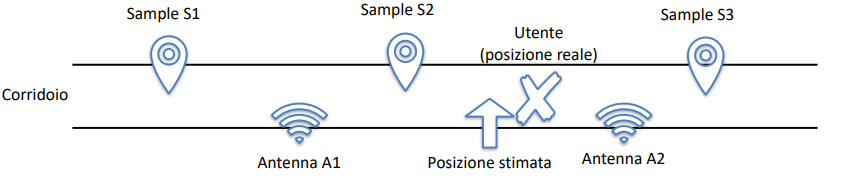
\includegraphics[width=\textwidth]{images/MobiDEV/1. posizionamento indoor/fingerprinting 3.PNG}
Si procede con il calcolo delle distanze da fingerprint in radio map, come nel caso precedente:
\begin{itemize}
    \item S1: $|$0,3-0,5$|$ + $|$0,7-0,01$|$ = 0,2 + 0,699 = 0,899
    \item S2: $|$0,3-0,4$|$ + $|$0,7-0,6$|$ = 0,1 + 0,1 = 0,2
    \item S3: $|$0,3-0,1$|$ + $|$0,7-0,8$|$ = 0,2 + 0,1 = 0,3
\end{itemize}
Successivamente stimo che la posizione dell'utente sia tra S2 ed S3 ad una distanza da S2 di 0,2 / (0,2+0,3) rispetto alla distanza totale tra S2 ed S3.

Abbiamo diversi problemi: la tecnica non è robustissima, abbiamo i dati che sono approssimativi, l'ambiente può cambiare (una porta che si apre o chiude influenza il radiomap), il numero di persone nell'ambiente influenza la radiomap, il tipo di antenna del device, l'umidità.

Bisogna avere quindi un sistema più robusto che riesca a gestire tutti questi fattori, quindi si usano tecniche probabilistiche o basate su machine learning (es: reti neurali).

C'è un altro problema, la fase di setup è molto onerosa. 
Ogni misurazione può durare anche decine di secondi. 
Ci sono vari modi per risolvere il problema:
\begin{itemize}
    \item interpolazione: l'incaricato parte da un certo punto, cammina con velocità regolare, il sistema misura la potenza del segnale e l'incaricato arriva al punto di destinazione. Il sistema sa interpolare i punti, avendo il punto di inizio e quello di fine e la velocità che è costante, l'applicazione calcola i vari fingerprint lungo il percorso
    \item robot: un sistema basato su ruote. In questo modo è più facile misurare lo spostamento. I robot esplorano l'ambiente, sappiamo quanto si spostano, in base a quanto girano le ruote
    \item crowdsourcing: non faccio fare la lettura all'incaricato ma faccio in modo che i dati vengano inseriti dagli utenti finali
\end{itemize}

\subsection{Le tecniche a confronto}

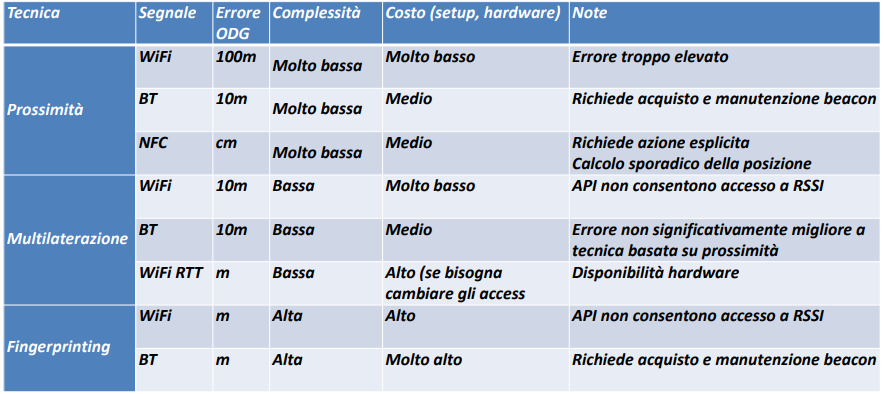
\includegraphics[width = \textwidth]{images/MobiDEV/1. posizionamento indoor/3 tecniche radio.PNG}

\begin{itemize}
    \item prossimità: hanno una minor precisione ma una maggior semplicità, hanno una costo ridotto
    \item multilaterazione: compromesso tra precisione e semplicità ma non aumentano in modo significativo la precisione
    \item fingerprinting: costo alto e complessità alta
\end{itemize}

\section{Sensori inerziali: calcolo dello spostamento}
Ci sono tecniche che permettono di calcolare la posizione come tecniche di dead reckoning utilizzate in diversi ambiti come in quello militare. Viene utilizzato un sommergibile che quando emerge, viene calcolata la posizione con GPS. Durante l'immersione, il segnale sotto una certa profondità non capisce più la posizione, per questo vengono sfruttati gli accelerometri che permettono di misurare l'accelerazione istantanea, dunque otteniamo lo spostamento. 

\textit{Si può usare in dispositivi mobili?}
\\ A bordo del sommergibile ci saranno accelerometri sicuramente più sofisticati rispetto ai telefoni. I sensori inerziali sono soggetti a meno rumore rispetto ad un telefono tenuto in mano mentre si cammina. 

Le tecniche inerziali vanno combinate con altre tecniche perché da sole non calcolano la posizione ma calcolano solo lo spostamento.
Un modo per rendere più robuste le tecniche è di combinare le tecniche inerziali con quelle visive. 

Se non conosco l'orientamento dell'utente, non serve a nulla sapere lo spostamento a meno che non usiamo filtri appositi.

\subsection{Gestione dell'errore}
Il sistema è soggetto a molte forme di errore:
\begin{itemize}
    \item potrebbe sbagliare a contare i passi o la loro lunghezza
    \item potrebbe sbagliare a calcolare la direzione
\end{itemize}
A differenza di tutte le altre tecniche, l’approssimazione nel calcolo della posizione cresce linearmente con il 
tempo. 
\\ Ad esempio ho un fix di posizione e orientamento a t=0s (errore zero). A t=2s mi aspetto un errore di posizione e orientamento contenuto: non posso aver sbagliato di tanto, in così 
poco tempo. A t=4s l’errore è dato dall’errore a t=2 più l’errore accumulato tra t=2 e t=4. Sarà sempre contenuto, ma 
generalmente maggiore dell’errore in t=2. A t=60s ho accumulato l’errore in tutti gli istanti precedenti, dunque generalmente avrò un errore ben più grande rispetto a t=2s.

Questo tipo di errore viene anche chiamato drift.

\subsection{Calcolare un passo}
In teoria è possibile calcolare quando l'utente fa un passo processando i dati di accelerometri e giroscopi. 
In termini pratici però sia iOS che Android rendono disponibile un sensore virtuale che calcola questa informazione (usando i dati di accelerometri e giroscopi), dunque è molto semplice ottenerla.
\\ Il limite di queste tecniche è che contano i passi, ma non si conosce la lunghezza del passo.
\\ Esistono diversi lavori finalizzati a calcolare la lunghezza del passo:
\begin{itemize}
    \item molti assumono che il device mobile sia solidale con il centro di massa dell'utente, come ad esempio lo smartphone legato alla cintura
    \item alcuni considerano il caso in cui il device sia tenuto in mano
    \item altri considerano che una persona faccia passi lunghi sempre uguali, in questo modo se conto i passi e so dove si sposta, posso imparare la lunghezza dei passi stessi da usare in futuro
\end{itemize}

\subsection{Tecniche visuo-inerziali}
Usando tecniche di computer vision è possibile stimare come si sta 
spostando-ruotando la camera.
Le tecniche visuo-inerziali combinano i dati dei sensori inerziali con la stima dello spostamento-rotazione ottenuta attraverso l’analisi del 
flusso video.
\\ Questo permette di ottenere una stima dello spostamento-rotazione 
più robusta rispetto al solo uso dei sensori inerziali.
\\ La tecnica è adottata dalle librerie esistenti di augmented reality.

\section{Tecniche ibride}
Combinano più soluzioni per cercare di avere una soluzione più affidabile.
\\ Un esempio di tecnica ibrida ne è il segnale radio usato in combinazione con la computer vision.
\\ Se ho due stanze identiche in piani diversi, con la tecnica computer vision risulta impossibile identificare la posizione esatta di un utente, per questo viene combinata con il segnale radio. 

Un'altra tecnica è l'utilizzo dei marcatori visivi con il calcolo della posizione. Non puoi chiedere ad un utente di spostarsi inquadrando sempre un marcatore, quindi uso i marcatori visivi. 
\\ Mentre l'utente si sposta uso le tecniche di spostamento, il problema è che dopo un po' la posizione non sarà più calcolata perfettamente, in quanto le tecniche di spostamento accumulino l'errore.
\\ Per azzerare l'errore, l'utente inquadra un marcatore visivo in modo tale che venga fatto anche un fix di posizione. 

\subsection{Tecniche ibride e calibrazione crowsourced}
In questo caso uso più tecniche di posizionamento. 
Quando una tecnica mi fornisce una posizione con buona approssimazione, ad esempio un utente inquadra un marcatore, oppure utente passa vicino ad un beacon, utilizzo questa informazione per calibrare le altre tecniche. Ad esempio tengo traccia della potenza delle antenne WiFi in quella precisa posizione.
Questo procedimento è analogo a quanto avviene in outdoor.


\chapter{Tecniche di aggregazione di dati soggetti a rumore}
\lhead{Tecniche di aggregazione di dati soggeti a rumore - MobiDEV}
\rhead{Lezione 3 - 8 marzo}
\begin{center}
    \textbf{--------- Lezione 3 - 6 ottobre 2020 ---------}
\end{center}

\section{Le reti cellulari}
Le reti cellulari permettono ad un dispositivo mobile di trasmettere voce e dati attraverso un'infrastruttura distribuita nel territorio composta da:
\begin{itemize}
    \item Antenne: sono sparse nel territorio ed ognuna di queste ha una copertura limitata. Per permettere ai dispositivi di avere una copertura sufficiente (una copertura geografica), ci sono molte antenne
    \item Varie componenti di elaborazione delle informazioni 
\end{itemize}

Nascono negli anni ’80 e si sono rapidamente evolute. Esempi di tecnologie: GSM, GPRS, EDGE, LTE.
\\ Queste tecnologie sono organizzate in generazioni (es. 1G, 2G, 3G, ecc.) dove ogni generazione stabilisce delle performance di riferimento. 
Le diverse tecnologie condividono una stessa architettura.

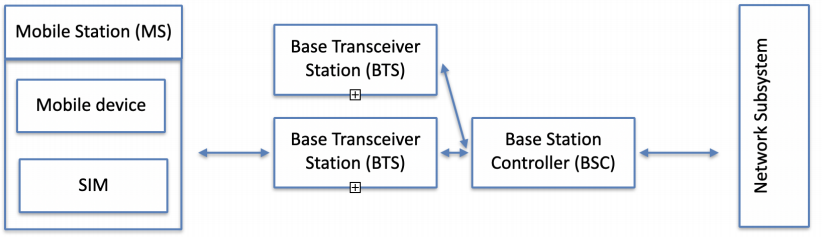
\includegraphics[width=\textwidth]{images/Mobile computing/3. Reti e architetture/architettura.PNG}

La \textit{SIM} è una componente HW che ha la scopo di identificare e autenticare l'utente per l'accesso alla rete. 
Le \textit{Mobile Station (MS)} includono due componenti: la SIM e il device.
La SIM contribuisce a funzioni di sicurezza in quanto contiene chiavi crittografiche utilizzate per realizzare la comunicazione di rete. 
\\ La mobile station comunica via radio con una componente chiamata \textit{Base Transceiver Station (BTS)} che include una o più antenne per la comunicazione e un hw di gestione dell'informazione per gestire il segnale in ingresso e in uscita. Ogni BTS è collegata al \textit{Base Station Controller (BSC)} che coordina varie BTS e a sua volta comunica con l'infrastruttura di rete chiamata \textit{Network Subsystem}. 

La potenza del segnale diminuisce all'aumentare della distanza tra la MS e l’antenna.
La distanza massima di comunicazione dipende dal tipo di tecnologia.
ma in linea di massima entro la quale si può comunicare è anche di diversi chilometri. 
Per erogare il servizio su una scala geografica, sono sparse nel territorio le BTS. 
Ciascuna BTS definisce una cella, cioè una regione geografica dove il segnale di quella BTS è più forte, rispetto al segnale delle BTS circostanti. 
Man mano che ci allontaniamo dall'antenna entriamo in un'altra cella perché il segnale di quest'altra antenna è più forte della precedente. 

Ogni BTS comunica con varie MS tramite onde radio, su intervalli di frequenze che sono specificati dal protocollo utilizzato.
Ogni intervallo è suddiviso in un numero finito di portanti che sono a loro volta suddivise in uplink e downlink (comunicazione verso la BTS).
Ad esempio GSM ha 248 portanti nell'intervallo attorno ai 900MHz.
\\ Ogni portante è suddivisa in canali usando tecniche di FDM (frequency division multiplexing) e TDM (time division multiplexing).
\\ Ogni MS nel momento in cui comunica con la BTS necessita di un canale in uplink e uno in downlink. Il numero massimo di MS che possono comunicare con una stessa BTS è limitato. 
In zone ad alta densità di popolazione è necessario avere celle più piccole, per suddividere la popolazione tra più BTS.
In questo caso una procedura, chiamata session handover, permette il passaggio di controllo di una mobile station ad un'altra e il dispositivo non si accorge di essere passato da un'antenna all'altra. L'IP del telefono rimane invariato. 

\section{Le architetture per dispositivi mobili}
Molto spesso le applicazioni di dispositivi mobili fanno parte di un sistema distribuito e comunicano con un server ed altri dispositivi mobili. 

Ci sono fattori che influenzano molto la progettazione della app:
\begin{itemize}
    \item la connessione potrebbe andare persa. Nei dispositivi mobili è anche normale che l'accesso ad Internet avvenga tramite diversi tipi di connessione che cambiano nel tempo
    \item il tipo di connessione cambia. In alcuni casi grazie al session handover è possibile mantenere la stessa connessione anche quando un dispositivo si sposta all'interno di una rete cellulare, ma la stessa funzionalità non è disponibile quando un dispositivo si sposta tra reti diverse e dunque riceve un nuovo indirizzo IP. Ad esempio un utente è connesso alla rete WiFi di casa, quando esce si connette alla rete cellulare e quando arriva a lavoro si connette ad un'altra rete WiFi che gli assegnerà un nuovo IP
\end{itemize}

\subsection{Connection-oriented vs connection-less}
I due fattori portano a sconsigliare l'utilizzo di protocolli connection-oriented dove si ha una connessione prolungata tra le due entità che comunicano.
Non è consigliabile perché il dispositivo perde la connessione e siccome ho una connessione aperta tra client server, se il client cambia l'indirizzo IP, la connessione va persa.

Nei protocolli connection-less invece non viene mantenuta una connessione prolungata tra due componenti. 
Queste comunicazioni sono più adatte ai dispositivi mobili. 

In un'architettura client-server, il server espone delle API (chiamate) che i client possono sfruttare per portare a termine il loro compito. 

\subsection{Architettura three-tier}
Lo schema architetturale three-tier è comunemente utilizzato per erogare servizi web. 
Il browser fa una richiesta HTTP al web server che legge e scrive i dati su un DB. Una volta che il web server termina la scrittura e la lettura dei dati, esegue lo script lato server, recupera il file necessario ed esegue il codice PHP che può richiedere di interagire con una base di dati. Il web server al browser ritorna la pagina html, il codice javascript che esegue lato client e dei css.
\\ PHP è lo scripting lato server e non viene eseguito lato client, javascript invece è lo scripting lato client e non viene eseguito lato server.

L'architettura per i dispositivi mobili è molto simile.
L'applicazione comunica con un web service tramite HTTP. Il web spesso comunica con un DB che memorizza l'informazione in modo persistente. 
Una delle differenza principali è che l'applicazione client
solitamente riceve dal web service solo i dati richiesti, in quanto il comportamento dell'applicazione, incluse le informazioni su come formattare i dati ricevuti, fanno già parte dell'applicazione stessa. I dati possono essere scambiati in un qualunque formato, incluso il testo semplice. Tuttavia, per dati complessi esistono vari formati, tra cui XML e JSON.

\begin{figure}
    \centering
    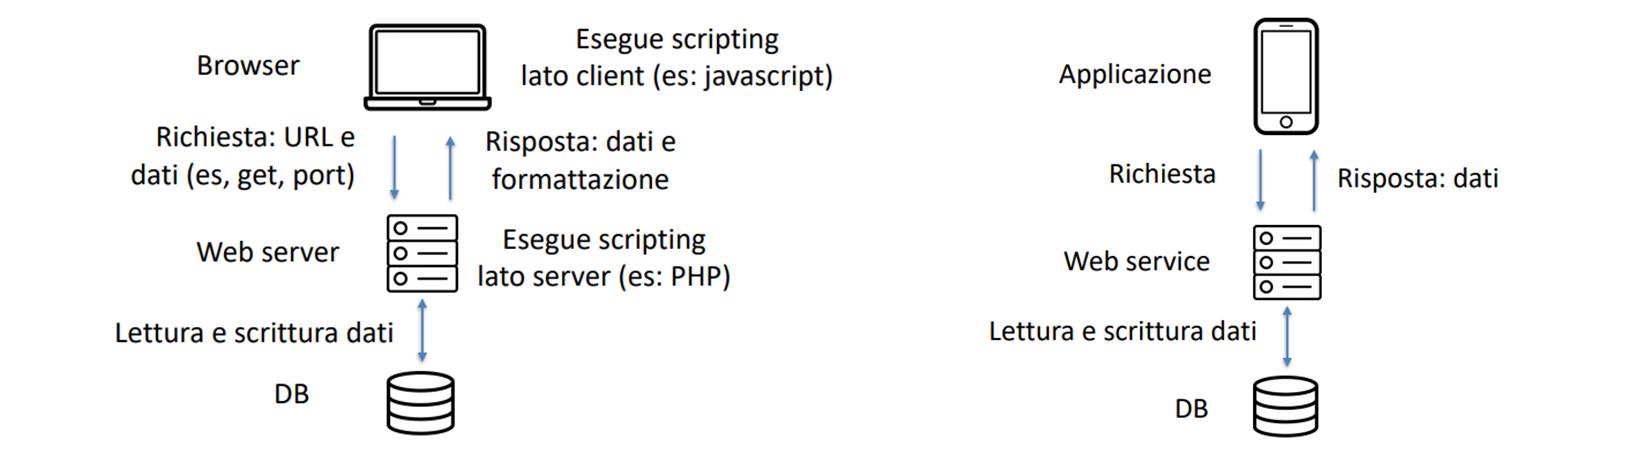
\includegraphics[width=\textwidth]{images/Mobile computing/3. Reti e architetture/architettura tt.png}
    \caption{Schema del modello three-tier applicato al web (sinistra) e alle applicazioni (destra)}
    \label{fig:architettura tt}
\end{figure}

I modelli presentano due componenti diversi:
\begin{itemize}
    \item web server: un server che fornisce informazioni (generalmente HTML+CSS+JS) finalizzate ad essere mostrate (tramite un browser) all'utente 
    \item web service: un server fornisce informazioni finalizzate ad essere ricevute da un’applicazione (anche mobile)
\end{itemize}

Quando facciamo un sistema vero, vogliamo far si che un sistema sia utilizzabile sia su app che su web e vorremmo evitare di scrivere due volte il codice.
Quello che si fa è usare un web server che manda tutti i contenuti al browser e che gli permettono di avere lo stesso comportamento dell'app mobile. 
\\ Invece di avere web service e web server, abbiamo un web service che interagisce con l'applicazione e poi il web server che passa semplicemente al browser la web app. 

\begin{figure}[!ht]
    \centering
    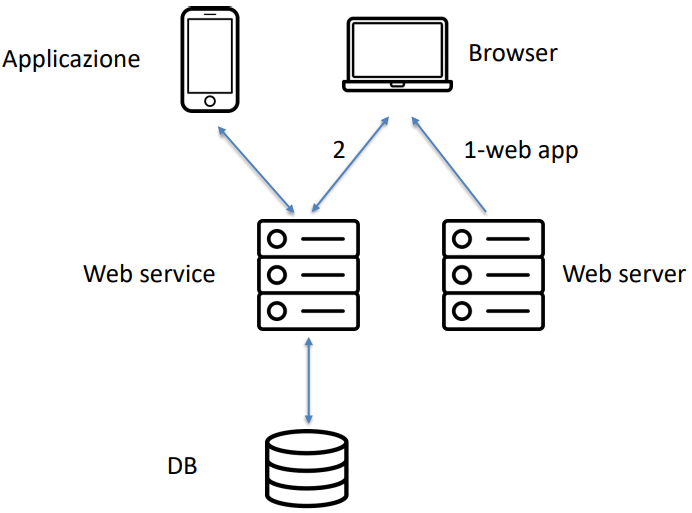
\includegraphics[width=.5\textwidth]{images/Mobile computing/3. Reti e architetture/app_web.PNG}
    \caption{Architettura per supportare contemporaneamente l'accesso da browser e da applicazioni}
    \label{fig:sistemi web_app}
\end{figure}

\subsection{La definizione del protocollo di comunicazione}
Progettare un protocollo di comunicazione non è facile. Vogliamo definire API sul server con le quali i client possono interagire: scambiare i dati con il server e ottimizzare il volume di dati scambiati, tenendo conto dei vincoli dei dispositivi mobili e permettendo una buona esperienza utente. 

Il protocollo è di tipo connection-less. Le chiamate avvengono con connessioni diverse, ma solitamente sono logicamente legate le une alle altre. Bisogna definire in quale ordine avvengono, in quali situazioni, quali dati si devono scambiare, ecc.

\subsubsection{Esempio di comunicazione}
Pensiamo ad un social. Ogni utente ha un profilo (con nome e foto) e uno stato (online o offline). Vogliamo che un utente possa scaricare la lista degli amici. 
\\ Il modo più semplice per implementare questa cosa è richiedere al server l'elenco dei contatti. 
È una soluzione semplice, ma ogni volta che l'utente vuole accedere alla lista, deve riscaricare tutti i contatti (con la foto, il nome e lo stato). 

Un'altra soluzione sarebbe di andare a scaricare in locale gli amici, in modo tale che una seconda volta scarico solamente quelli che precedentemente non avevo ancora scaricato (ad esempio un nuovo amico).
Qui ho un altro problema, perché se un amico aggiorna la foto profilo, io in locale ho quella vecchia. 

La soluzione corretta e ottimizzata è quella di utilizzare un contatore. Per ogni utente il server gestisce un contatore delle foto di profilo caricate (un numero di versione). Quando un utente scarica l’elenco degli amici il server gli manda, per ciascuno, il numero di versione della foto (è un dato di dimensione irrilevante rispetto ad un’immagine). Per ogni amico verifico se ho già salvato in locale la foto giusta e nel caso la mostro, altrimenti chiedo la foto al server e poi la salvo in locale per la prossima volta.

\begin{figure}[!ht]
\begin{center}
    \subfloat[Aggiornamento delle foto]{\fbox{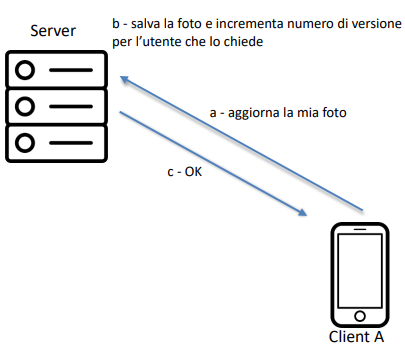
\includegraphics[width=.4\textwidth]{images/Mobile computing/3. Reti e architetture/1.PNG}}}
    \qquad \subfloat[Scarico lista amici]{\fbox{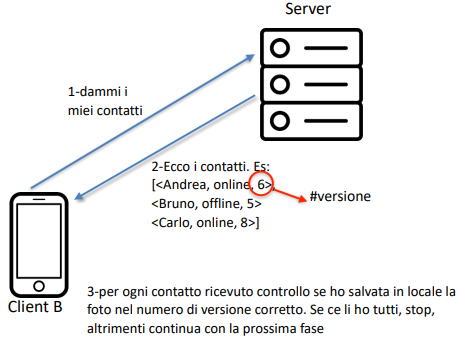
\includegraphics[width=.45\textwidth]{images/Mobile computing/3. Reti e architetture/2.PNG}}}
    
    \subfloat[Scarico foto aggiornate]{\fbox{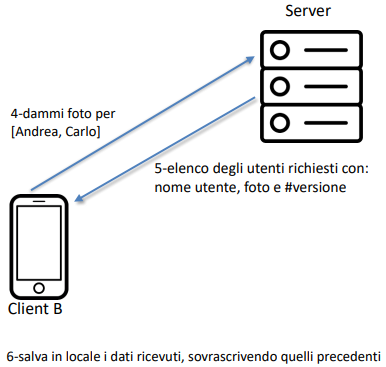
\includegraphics[width=.4\textwidth]{images/Mobile computing/3. Reti e architetture/3.PNG}}}   
\end{center}
\caption{Trasmissione delle immagini profilo in un social network}
\label{fig:immagini social}
\end{figure}
\newpage

\section{La codifica dell'informazione}
In una richiesta HTTP è possibile trasmettere informazioni in testo semplice. 

Prendiamo ad esempio un servizio che prende una parola in input e risponde con un sinonimo.
L'output è sempre una stringa e se non viene trovata nessuna corrispondenza, ritorna la stringa vuota.

Prendiamo ad esempio, invece, un servizio che data una parola in input risponde con una lista sinonimi. 
In questo caso potremmo ad esempio usare una codifica di parole separate da virgole. 

Diventa peggiore se data una parola in input, risponde con una lista di sinonimi e una di contrari.
Dobbiamo rappresentare due liste di parole e potemmo inventarci un modo per separare le due liste, per esempio usare il punto e virgola per separare.

Esistono degli strumenti che ci permettono di codificare l'informazione come ad esempio XML e JSON.

XML è un linguaggio di markup che permette di definire formati dei dati che sono “human and machine readable”. 

Un documento XML è ben formattato se rispetta alcune regole (ad esempio se tutti i tag sono aperti e poi chiusi). 
XML presenta alcuni limiti:
\begin{itemize}
    \item tende ad essere verboso 
    \item non facilmente leggibile da umani
    \item gli schemi XML sono abbastanza difficili da definire e spesso vengono ignorati
\end{itemize}

Un esempio di risposta XML per il servizio dictionary:
\begin{XML}
    <dictionary entry="nice">
        <synonyms>
            <word>pleasant</word>
            <word>agreeable</word>
            <word>enjoyable</word>
        </synonyms>
        <antonyms>
            <word>ugly</word>
            <word>unpleasant</word>
        </antonyms>
    </dictionary>
\end{XML}

JSON concettualmente svolge lo stesso lavoro di XML, cerca di ridurre la verbosità e di migliorare la lettura. 
\\ Un esempio di risposta JSON per il servizio dictionary:
\begin{JSON}
    {
        "entry":"nice",
        "synonyms ":[" pleasant","agreeable","enjoyable"],
        "antonyms ":[" ugly","unpleasant"]
    }
\end{JSON}    

XML definisce delle entità, JSON definisce degli oggetti. 
Sono due rappresentazioni diverse, ma concettualmente sono analoghi, infatti rappresentano i dati di un elemento che vogliamo descrivere.

Un'entità in XML o un oggetto JSON mi definisce uno stato nel mondo reale ma non il comportamento, nei linguaggi di programmazione invece un oggetto definisce sia lo stato che il comportamento ad esso associato. 
Questa distinzione è molto importante in quanto esiste una forte correlazione tra le strutture dati dei programmi e la codifica in XML o JSON. 

\subsection{Serializzazione e deserializzazione}
In memoria principale lavoriamo con oggetti dei linguaggi di programmazione ma questi oggetti non possono transitare in rete. Quello che ci serve è andare a convertirli nella propria rappresentazione XML o JSON. Questa operazione si chiama \textit{serializzazione} (o \textit{marshalling}). Il risultato è una stringa (internamente codificata in XML o JSON). L'entità che riceve la comunicazione di rete può leggere questa stringa e
riconvertirla in struttura dati tramite un’operazione che si chiama \textit{deserializzazione} o \textit{unmarshalling}.
Uno dei vantaggi nell'uso di XML o JSON è che le operazioni di serializzazione e deserializzazione sono supportate, in quasi tutti i linguaggi di programmazione, da apposite librerie.
Un esempio di queste librerie è GSON. 
\\ GSON è lo strumento di conversione, JSON è il formato di rappresentazione.

\subsection{Codifica di dati binari}
Sia in XML che in JSON vengono rappresentati i dati singoli nella loro codifica testuale. Non c'è nessun problema per stringhe, interi, float, boolean, ecc, ma si pone un problema per i dati binari ad esempio le immagini.
Il modo più comune è la codifica Base64 che permette di rimappare la codifica binaria dell'informazione in alcune informazioni testuali.
\\ Definisco una conversione tra 64 simboli (caratteri ASCII) e un valore numerico: A=1, B=2, ecc.
Scelgo dei caratteri ASCII che non mi introducano confusione nelle rappresentazioni XML o JSON (es: non uso "$<$", né ",").
Un simbolo rappresenta dunque 6 bit ($2^6$ = 64).
Dunque per rappresentare 3 byte in binario mi servono 4 simboli (3*8 = 4*6).
Per convertire da binario a Base64 suddivido l’input in gruppi di 3 byte, codifico ciascun gruppo con 4 simboli Base64.
Si usa la Base64 perché è una codifica testuale che usa meno caratteri per rappresentare e perché permette di non utilizzare caratteri strani. 

\subsection{Protocol Buffer}
Protocol Buffer è il protocollo definito da Google per serializzare le informazioni. Risolve lo stesso problema di XML e JSON definendo non solo il formato di scambio, ma anche gli strumenti SW di (de)serializzazione.
\\ Protocol Buffer è un protocollo:
\begin{itemize}
    \item multi-piattaforma, multi-linguaggio 
    \item ottimizzato in termini di dimensione del messaggio da scambiare 
    \item che risolve diversi problemi tipici ad esempio la gestione della versione dei protocolli 
\end{itemize}
\vspace{2em}

\chapter{Augmented Reality}
\lhead{Augmented Reality - MobiDEV}
\rhead{Lezione 4 - 11 marzo}
Non è sufficiente far comunicare i processi in un sistema distribuito per realizzare le funzionalità del sistema. Ci serve praticamente sempre una qualche forma di coordinamento tra le computazioni che ci sono nei vari nodi e quindi coordinare anche le comunicazioni che occorrono per raggiungere gli obbiettivi.

Gli algoritmi di sincronizzazione prevedono uno scambio di messaggi (solo in questo modo i nodi possono parlare e organizzare il loro coordinamento).

\section{Clock Synchronization}

All'interno di un sistema distribuito, ogni nodo è indipendente ed ha quindi un proprio clock interno. Questo clock non è perfetto. Quando ogni macchina ha il proprio clock, un evento che si è verificato dopo un altro evento può comunque essere assegnato ad un timestamp precedente, dunque i sistemi non possono semplicemente basarsi sul confronto dei timestamp.

\section{Physical Clocks}

Non è possibile sincronizzare perfettamente gli orologi, poiché ci sono i tempi di latenza della rete. Possono, però, essere sincronizzati con un certo livello di approssimazione rispetto al tempo preciso. Il riferimento principale è l'UTC.

Il modo in cui noi misuriamo il tempo deriva dall'osservazione di fenomeni astronomici. Di fatto, il tempo è la distanza tra due eventi. Gli orologi comuni dividono il giorno solare medio basandosi sull'oscillazione dei cristalli di quarzo. L'orologio atomico, invece, misura il tempo in termini di transizioni di un atomo di Cesio 133. Dal giorno solare medio viene derivato il secondo solare medio, che corrisponde a circa 9 miliardi di transizioni di Cesio.

Una serie di istituti per la misurazione del tempo, che hanno degli orologi atomici, si accordano tra di loro, facendo una media, dopodiché delle stazioni si occupano di distribuire questo tempo quasi perfetto (TAI). Il TAI non è comunque perfettamente preciso, poiché l'universo non è regolare (la rotazione della Terra diminuisce, i fenomeni astronomici mutano, etc). Dunque, questi istituti, quando si accorgono che ci si sta discostando dall'osservazione astronomica, aggiungono dei secondi chiamati leap seconds che non sono periodici. Questo di solito viene fatto a capodanno.

UTC = TAI + leap seconds

L'ideale è che i nodi di un sistema distribuito corrispondano tutti all'UTC, ma questo non è possibile. Nella realtà, tutti gli orologi saranno più lenti o più veloci, quindi dovranno essere sincronizzati più o meno frequentemente in base a quanto divergono dal perfect clock.

\section{Synchronizing Physical Clocks}

\subsection{GNSS}

È possibile utilizzare i GNSS per ottenere il tempo, poiché i satelliti dei sistemi GNSS hanno a bordo degli orologi atomici. Ogni satellite di un GNSS fa un broadcast di messaggi che contengono il timestamp dell'orologio atomico (nel momento in cui viene inviato il messaggio), oltre all'identificatore del satellite stesso. Il ricevitore ascolta più satelliti e usa metodi di geometria computazionale per determinare la propria posizione (dimensione spaziale) e una dimensione temporanea. Il tempo ottenuto dal GNSS ha una precisione dell'ordine dei micro o addirittura dei nanosecondi (ma dipende in realtà dalla precisione del GNSS).

Il GPS è il sistema di navigazione satellitare globale (GNSS) più utilizzato e riesce a calcolare la posizione guardando quanto tempo impiega il segnale ad essere trasmesso dal satellite al ricevitore e capendo a quante unità di distanza si trova, da qualche parte su una circonferenza. Ricevendo la posizione da un secondo satellite riduce le possibili soluzioni a due punti, ed aggiungendo un terzo satellite deduce più facilmente quale dei due possa essere. Dunque, se il nodo del sistema distribuito ha un GPS, allora ha già un modo per sincronizzarsi in maniera abbastanza precisa con l'UTC. 

Complicazioni del GPS:
\begin{itemize}
    \item ci vuole del tempo prima che i dati sulla posizione di un satellite raggiungano il ricevitore. 
    \item l'orologio del ricevitore generalmente non è sincronizzato con quello del satellite.
    \item la precisione del GPS è principalmente disturbata nel caso in cui il segnale faccia fatica ad arrivare, anche a causa di fenomenti metereologici. Esistono metodi di aggiustamento che si appoggiano a delle stazioni a terra che, osservando i fenomeni metereologici, forniscono l'aggiustamento. 
\end{itemize}

\subsection{Cristian’s algorithm and Network Time Protocol}

Se un nodo del sistema distribuito non ha un GPS, il metodo più comune è rivolgersi ad un server. L'algorimo NTP deriva dall'algoritmo di Cristian: si ispira a quello, ma è stato perfezionato per riuscire a stimare meglio i ritardi dovuti alla rete. 

Non prevede una banale architettura client-server, bensì prevede una gerarchia di server NTP divisi per strato. Lo strato 1 riguarda gli NTP server che hanno un orologio atomico o sono collegati ad esso con una rete a latenza bassissima. Gli strati inferiori, invece, garantiscono meno precisione. 

Il client fa una richiesta ad un server NTP, supposto avere un'ora più o meno precisa, chiedendo l'UTC. L'aspetto complicato di questo algoritmo è calcolare le latenze.  L'idea è che nel messaggio di richiesta venga inserito anche il timestamp. Conoscendo i timestamp di invio/ricezione della richiesta/risposta, può essere calcolata la distanza tra invio e ricezione della richiesta e la distanza tra invio e ricezione della risposta, dividendo per 2 (approssimazione, non è detto che siano uguali). Per fare un'approssimazione migliore di queste latenze, viene ripetuta l'operazione più volte. NTP permette di raggiungere un'accuratezza nell'ordine dei millisecondi.

\subsection{Berkeley Algorithm}

Fino a qui abbiamo visto due metodi (più utilizzati) per effettuare la sincronizzazione con il tempo reale. Non tutti i sistemi, però, hanno bisogno di questo. Se il sistema deve interagire con misure provenienti dal tempo reale, allora è opportuno, in altri casi, quando il sistema è chiuso, potrei anche accontentarmi del fatto che i nodi siano semplicemente tutti sincronizzati su un tempo.

Uno dei nodi funziona da Time Daemon e manda a tutti quanti (anche a se stesso) il proprio orario. I nodi rispondono con la differenza del loro orologio rispetto a quello che hanno ricevuto. Il Time Daemon calcola quindi una media tra gli orari e comunica a tutti di sistemarsi su questa media. 

Non importa che sia l'orario vero oppure no e spesso questo algoritmo viene utilizzato in un ambiente ristretto, dove i nodi sono collegati attraverso una banda larga, per cui la latenza non viene solitamente presa in considerazione. Attenzione, però, che portare indietro un orologio non è una cosa indolore. Quello che avviene, di fatto, è farlo rallentare finché non è allineato, come se fosse stato portato indietro.

\section{Lamport’s Logical Clocks}

In molti casi non è necessario che i nodi concordino sul valore dei loro orologi fisici, bensì è possibile semplicemente utilizzare dei contatori o degli orologi logici (possono essere immaginati come dei contatori). Questo è possibile quando nel sistema distribuito è sufficiente avere una conoscenza condivisa sull'ordine parziale degli eventi, cioè quando occorre che il sistema sappia cosa è accaduto prima/dopo di qualcos'altro. 

Un evento può essere:
\begin{itemize}
    \item evento interno: ogni nodo ha un processo in esecuzione e ci sono eventi che riguardano processing locale
    \item messaggio inviato/ricevuto
\end{itemize}

Il tempo aumenta sempre, dunque utilizzando un contatore con questa stessa proprietà, otteniamo un clock logico. All'interno di ogni nodo viene utilizzato un contatore intero come orologio logico e viene incrementato ogni volta che si verifica un evento interessante (inizialmente saranno tutti uguali a 0). Osservando lo stato del sistema, in un particolare istante, si potrà notare che gli orologi logici avranno valori diversi. 

L'algoritmo di Lamport prevede che:
\begin{itemize}
    \item se A e B sono due eventi, l'espressione A $\rightarrow$ B denota la relazione (transitiva) A accade prima di B
    \item C(A) è il valore di clock logico assegnato dal processo in cui si verifica A
    \item Obiettivo: se A $\rightarrow$ B, allora C(A) $<$ C(B), anche se sono su due processi diversi
\end{itemize}

Se A e B sono eventi sullo stesso processo, il contatore viene semplicemente incrementato. Il problema si pone nel momento in cui A è l'evento di invio da un nodo e B è l'evento di ricezione su un altro nodo. Potrebbero verificarsi molti eventi prima di A e pochi eventi prima di B, avendo così C(A) maggiore di C(B). Ovviamente questo comportamento non va bene, dunque:

\begin{itemize}
    \item prima di eseguire un evento, incremento il contatore
    \item quando il processo Pi manda un messagio m a Pj, inserisce il valore del contatore dopo l'incremento
    \item Pj riceve il messaggio m, osserva il valore del contatore e lo confronta con il proprio. Dopodiché prende il maggiore e lo incrementa di uno
\end{itemize}

Questo, così come tutto ciò che vediamo nei sistemi distribuiti, si implementa attraverso un middleware.

\subsection{Enforcing Total Order}

Alcuni algoritmi vorrebbero un ordinamento totale dei timestamp nel sistema. Per evitare che due valori di clock nel sistema per due eventi diversi siano uguali, viene concatenato l'identificatore del processo (un qualsiasi numero che difficilmente si trovi in altri processi) al contatore. A questo punto, prendendo due valori di timestamp, è possibile stabilire un ordine totale tra questi: si osserva il valore di contatore maggiore/minore e, in caso di uguaglianza, si osserva l'identificatore maggiore/minore. L'obiettivo, quindi, è che ogni evento del sistema abbia associato un timestamp diverso. Attenzione, però, che un ordine totale dei timestamp non significa conoscere la relazione temporale tra ogni coppia di eventi.

\section{Totally Ordered Multicast}

Si assume che nessun messaggio venga perso e che i messaggi dallo stesso mittente vengono ricevuti nell'ordine in cui sono stati inviati.

Il processo Pi invia un messaggio m\textsubscript{i} con un timestamp a tutti gli altri. Il messaggio stesso viene inserito in una coda locale i. Qualsiasi messaggio in arrivo su Pj viene accodato nella coda j, in base al suo timestamp, e viene inviato un ack di ricezione del messaggio ad ogni altro processo (gli eventi di invio e ricezione di messaggi e ack sono totalmente ordinati con Lamport). Pj passa un messaggio m\textsubscript{i} alla sua applicazione se:
\begin{itemize}
    \item m\textsubscript{i} è in testa alla coda j AND
    \item m\textsubscript{i} è stato confermato da tutti gli altri processi 
\end{itemize}

Tutti i processi alla fine avranno la stessa copia della coda locale, quindi tutti i messaggi vengono passati all'applicazione nello stesso ordine ovunque.

\section{Mutual exclusion}

In un sistema distribuito, se un insieme di processi in esecuzione su sistemi diversi vogliono accedere ad una risorsa condivisa, occorre effettuare uno scambio di messaggi.

\subsection{A centralized algorithm}

Un processo, su uno dei nodi, viene utilizzato per gestire la coda. Gli altri nodi, con la solita modalità client/server, se necessitano di accedere alla risorsa lo richiedono al coordinatore. Se la coda è vuota, il coordinatore consente l'accesso, altrimenti il coordinatore non risponde (si suppone che sia sincrono, per cui il processo si blocca) ed inserisce la richiesta in coda. Nel momento in cui il coordinatore riceve il release da parte del processo che stava utilizzando precedentemente la risorsa, estrae la prima richiesta dalla coda (FIFO) e consente l'accesso. Il processo, a questo punto, si sblocca e riceve la possibilità di utilizzare la risorsa fino a che non la rilascerà. 

I problemi di questo algoritmo sono:
\begin{itemize}
    \item single point of failure: in caso di crash del coordinatore nessuno potrà più accedere alla risorsa, a meno che non sia replicato in qualche modo
    \item se l'utente non rilascia la risorsa, occorre un meccanismo di timeout (tempo limite di rilascio) dopo il quale viene tolta forzatamente
    \item bottleneck: passano tutti per lo stesso coordintore
\end{itemize}

\subsection{A distributed algorithm}

Si assume un ordinamento totale dei timestamp e una consegna affidabile dei messaggi, attraverso un meccanismo di ack. 

Un processo P che vuole accedere ad una risorsa costruisce un messaggio contenente il nome della risorsa, l'id del processo ed il timestamp corrente (contatore + identificatore) e dopodiché invia il messaggio a tutti i processi, incluso se stesso.  Quando un processo Q riceve un messaggio, abbiamo 3 casi:

\begin{itemize}
    \item se Q non sta utilizzando R e non ha intenzione di farlo, risponde OK a P
    \item se Q sta utilizzando R non risponde e accoda la richiesta
    \item se Q non sta utilizzando R, ma ha intenzione di farlo, confronta il timestamp del messaggio con quello della propria richiesta. Se quello nel messaggio inviato da P è inferiore risponde OK a P, altrimenti accoda il messaggio
\end{itemize}

Dopo aver inviato il proprio messaggio, P attende un OK da tutti i processi prima di accedere a R. Quando P termina di utilizzare R, invia OK a tutti i processi che aveva precedentemente inserito nella sua coda e la svuota.

Si potrebbe anche ipotizzare di utilizzare l'orologio fisico, ma, anche se fossero sincronizzati correttamente, ci si potrebbe comunque trovare nella situazione di avere più volte uno stesso timestamp, andando ad invalidare l'assunzione, a meno che non si aggiunga al timestamp l'identificatore del processo.

I problemi di questo algoritmo sono:
\begin{itemize}
    \item la mancata risposta da parte di un processo può essere dovuta ad un suo crash
    \item coinvolgere tutti i processi di un sistema distribuito optrebbe essere uno spreco di risorse (con l'aumentare dei nodi)
\end{itemize}

\subsection{A ring algorithm}

Questo algoritmo utilizza una rete di collegamento tra i nodi che non rispecchia la rete di collegamento fisica. Partendo da un gruppo di processi non necessariamente ordinati viene costruito un anello logico, assegnando un identificatore univoco a ciascun processo in esecuzione sui diversi nodi del sistema. Dopodiché viene utilizzato un token, rappresentato da un messaggio, per gestire l'accesso alla risorsa. Il token viene fatto ruotare all'interno dell'anello e chi lo ottiene acquisisce la possibilità di accedere alla risorsa. Essendocene uno solo, non potrà mai essere in due nodi contemporaneamente. Quando il processo termina di utilizzare la risorsa passa il token al processo successivo. Non può usare due volte lo stesso token.

I problemi di questo algoritmo sono:
\begin{itemize}
    \item nel caso in cui si dovesse avere il crash di uno dei nodi si spezzerebbe l'anello. Solitamente per avere un po' più di tolleranza si memorizzano k elementi in avanti
    \item perdita del token
\end{itemize}

%TODO: inserire tabella comparativa

\section{Election algorithms}

Questi algoritmi prevedono una modalità con la quale un insieme di nodi si accorda su quale sarà il coordinatore, eleggendo il processo attivo (in qualsiasi istante potrebbe non esserlo più) con l'identificatore più alto in quel momento. Alcuni algoritmi presumono che ogni processo conosca gli ID e possa comunicare con qualsiasi altro processo. Tuttavia, non possono sapere se un processo è attivo. 

Questi algoritmi non perdono di generalità: può essere creato un ordinamento totale utilizzando il criterio che si ritiene più opportuno nella realizzazione degli identificatori.

\subsection{Bully Algorithm}

Abbiamo un gruppo di processi, di cui uno con l'identificatore più alto. Nel momento in cui un processo, dopo aver tentato di comunicare con il coordinatore, si accorge che questo non è più attivo (timeout scaduto), indice un'elezione, inviando un messaggio a tutti i processi con ID maggiore del proprio (compreso il coordinatore precedente, che nel frattempo potrebbe essere tornato disponibile), non sapendo se questi sono attivi. Quando un processo attivo riceve un messaggio di elezione, risponde con un messaggio di OK. Se un processo riceve almeno un OK, esce dall'elezione, poiché vuol dire che c'è almeno un processo con l'ID più alto del suo che si occuperà dell'elezione. A questo punto, i processi che hanno dato l'OK manderanno nuovamente un messaggio di elezione ai processi con identificare più alto del loro, ripetendo la stessa procedura vista precedentemente. Alla fine, il processo che non riceverà alcuna risposta entro un certo timeout diventerà il coordinatore e manderà un messaggio in broadcast per informare gli altri nodi.

Potrebbero essere indette più elezioni contemporaneamente, ma di solito dovrebbe vincere lo stesso nodo.

\subsection{A ring-based election:\\ Chang and Roberts algorithm (1979)}

Questo algoritmo utilizza una struttura ad anello, in cui i messaggi circolano in senso orario, senza fallimenti, e in cui i processi hanno un identificatore unico. L'obiettivo è eleggere il processo attivo con l'ID più alto (deve essere unico, anche nel caso in cui più elezioni siano indette in modo concorrente).

L'algoritmo funziona nel seguente modo:

\begin{itemize}
    \item i processi sono contrassegnati da un valore booleano che indica se questi sono partecipanti o non, in maniera tale da poter fermare il prima possibile eventuali messaggi di altre elezioni che porterebbero allo stesso risultato
    \item inizialmente tutti i processi sono contrassegnati come non partecipanti 
    \item quando un processo Pk si accorge che il coordinatore non sta più rispondendo, indice un'elezione contrassegnandosi come partecipante e inviando al nodo successivo nell'anello un messaggio $<$ELECTION, ID(Pk)$>$
    \item quando un processo Pm riceve un messaggio $<$ELECTION, ID(Pk)$>$:
    \begin{itemize}
        \item se l'ID del processo Pk contenuto nel messaggio è maggiore dell'ID del processo Pm, inoltra il messaggio al processo successivo nell'anello e si contrassegna come partecipante
        \item  se l'ID del processo Pk contenuto nel messaggio è minore dell'ID del processo Pm, si contrassegna come partecipante e sostituisce l'ID presente nel messaggio con il proprio, inoltrandolo poi al processo successivo nell'anello. Se, invece, il processo era già contrassegnato come partecipante, ferma il messaggio, bloccando così l'elezione
        \item se l'ID del processo contenuto nel messaggio è il proprio, vuol dire che non c'è nessun altro processo attivo con ID più grande. Si contrassegna, quindi, come non partecipante ed invia un messaggio $<$ELECTED, ID(Pm)$>$ al processo successivo nell'anello
    \end{itemize}
    \item quando un processo Pk riceve un messaggio $<$ELECTED, ID(Pm)$>$, si contrassegna come non partecipante, memorizza l'ID del coordinatore e, a meno che non sia lui stesso il coordinatore, inoltra il messaggio al processo successivo nell'anello
\end{itemize}

I problemi di questo algoritmo sono:

\begin{itemize}
    \item Errori di gestione: gli errori dovuti al crash dei nodi nell'anello vengono gestiti da ciascun processo memorizzando, non solo l'indirizzo del processo successivo, ma anche alcuni altri che lo seguono nell'anello. Se la comunicazione con il processo successivo fallisce, il messaggio viene inviato al primo tra quelli che lo seguono che è attivo
    \item Elezioni simultanee: l'uso dello stato partecipante/non partecipante aiuta a estinguere il prima possibile i messaggi non necessari nelle elezioni simultanee 
\end{itemize}

Nel caso peggiore vengono scambiati 3n - 1 messaggi, cioè quando il coordinatore dovrebbe essere il nodo appena prima di quello che ha indetto l'elezione.

Il caso peggiore si verifica quando il processo con l'ID più alto è il processo più vicino in senso antiorario a quello che indice l'elezione. In questo caso abbiamo bisogno di N - 1 messaggi per raggiungere il nodo, altri N messaggi per concludere l'elezione e N messaggi per annunciare il coordinatore, dunque 3N - 1. 

%TODO: inserire immagini

























\begin{comment}
---------------
Fabio

Problemi di sincronizzazione:
(uno degli aspetti fondamentali dei sistemi distribuiti). Serve una forma di coordimento tra le computazioni tra i nodi. Far comunicare un processo nell'ambiente dei sistemi distribuiti necessita di determinate tecnologie (socket, rpc..). 


Clock synchronization:
Problema tempo sistema distribuito: ogni nodo è indipendente e ha un suo clock interno. QUesto clock non è perfetto. Se ogni macchina ha il proprio clock con la propria precisione, ci si può trovare in situazioni strane ad esempio viene timpstampato ad un tempo precedente o futuro da quello effettivo. Basarsi su di un confronto di orologi diventa impossibile se hanno tempi diversi di clock. Come faccio a tenere gli orologi allineati?

Clock fisico:
E' possibile sincronizzare in maniera perfetta gli orologi di due diversi nodi? NO. Perchè ci sono i tempi di latenza di rete, sia che siano tanto distanti sia che siano sotto la stessa rete interna. Dunque si possono sincronizzare in maniera approssimata. 
L'UTC è lo standard di tempo che viene utilizzato dai calcolatori. L'UTC viene dalla misurazione dei fenomeni astrologici. Più specificatamente utilizziamo il giorno solare medio. 

UTC = TAI + leap seconds
Il tempo preciso viene preso con degli orologi atomici che misura il tempo in termini di transizioni di un atomo di cesio 133. (TAI)
Comunque il TAI non è preciso perfettamente perchè l'universo non è regolare. La rotazione della terra diminuisce, i fenomeni astronomici mutano etc etc. Dunque bisogna controllare che il tempo sia sempre allineato con i fenomeni astrologici. Ecco che vengono utilizzati dei leap seconds (che solitamente vengono aggiunti a capodanno) che servono per aggiustare il tempo. 

Clock veloci e lenti:
Dunque l'ideale sarebbe che tutti i nodi del sistema distribuito avessero tutti l'UTC, ma non è possibile.  

Synchronizing phisical clocks:
[GPS] 1°
Un modo di sincronizzare gli orologi fisici è il GPS. Il dispositivo ha un ricevitore (GPS) che riceve il segnale inviato da diversi satelliti. Insieme alla posizione è possibile avere anche il tempo preciso perchè i satelliti del GNSS hanno a bordo orologi atomici. I satelliti hanno a bordo orologi atomici per calcolare la posizione guardando il tempo che ci mette il segnale a raggiungere il dispositivo in ascolto. Dunque se il nodo nel sistema distribuito ha un GPS allora si ha un modo per sincronizzarsi con l'UTC usando il segnale dei satelliti.

Global Positionig System:
Cosa disturba il segnale che arriva al GPS?
essere indoor, sotto terra, dove ci sono palazzi alti etc...
Ma più importante i fenomeni metereologici. Dunque i sistemi si appoggiano a delle stazioni a terra che utilizzano i fenomeni meteorologici per calcolare l'errore

[NTP] 2°
Se non si ha un GPS il metodo più comune è quello di rivolgersi ad un Server. L'algoritmo NTP si ispira all'algoritmo di Cristian. NTP prevede una gerarchia di server NTP. Lo strato 1 riguarda gli NTP server che hanno un orologio atomico o sono collegati ad un orologio atomico. Negli strati inferiori invece garantiscono meno precisione. 
Il client fa una richiesta al server. Il server risponde con l'UTC. Problema, latenza tra le richieste. Idea: quando si manda il messaggio di richiesta si inseriscono i timestamp. Così si riesce a fare calcoli matematici basati sui timestamp per stimare i ritardi. NTP ripete la procedura più volte per approssimare in maniera migliore. NTP prevede di raggiungere un'accuratezza nell'ordine dei millisecondi. 

Non tutti i sistemi hanno bisogno di utilizzare il tempo reale. Ad esempio quando un sistema è chiuso è bene pensare che sia importante avere tutti i nodi che sono sincronizzati su un tempo che può anche non corrispondere a quello reale.
Metodo che viene utilizzato in questo caso:

[Algoritmo Berkeley] 3°
Ipotesi: Uno dei server funge da time deamon. Il protocollo manda a tutti quanti l'orario del deamon. I nodi rispondono con la differenza tra la loro ora e quella ricevuta. (ignoriamo la latenza per l'esempio). Il server calcola una media tra tutti gli orari e ridistribuisce un orario a tutti i nodi. Spesso questo algoritmo si usa in un ambiente ristretto dove i nodi sono collegati con una banda larga e per quello la latenza non viene solitamente presa in considerazione.

Lamport's Logical Clocks
In alcuni casi è possibile semplicemente utilizzare degli orologi logici. Dunque si lasciano gli orologi veri invariati e al posto loro vengono utilizzati dei "contatori" per sincronizzare i nodi. Questo può essere utile perchè in alcuni casi è sufficiente avere una conoscenza distribuita (condivisa) da tutti i nodi sull'ordine di determinati eventi e non tutti.
EVENTO: un evento è mandare/ricevere un messaggio (in questo caso)
Viene utilizzato un contatore (relazionato con il tempo grazie alla proprietà che va sempre in avanti) che viene chiamato clock logico. Principio: Inizio tutti 0, ogni qualvolta che succede un evento, il contatore viene incrementato. Quando si guarda l'intero sistema in un determinato momento del tempo reale, si ha che gli orologi logici sono differenti. Dunque l'algoritmo di Lamport dice che se A e B sono eventi, L'espressione a --> b denota che la relazione a è avvenuta prima di b. La relazione è transitiva
...
... [vedere slide]
...

Enforcing total order
Ci sono degli algoritmi in cui sarebbe utile avere un ordine totale dei timestamp nel sistema. Per evitare che ci siano due valori di clock per due eventi del sistema che sono uguali, si aggiunge al contatore un identificatore (può essere qualunque numero che risulta difficile da trovare in qualsiasi processo). Così facendo, prendendo due qualsiasi valori di timestamp (contatori + identificatore) si può stabilire un ordine totale tra i due. Come si fa? Si controlla il valore del contatore e, nel caso di uguaglianza, si controlla l'identificatore.
Un ordine totale nei timestamp non significa conoscere la relazione temporale tra ogni coppia di eventi, ma conoscere quelli che sono legati dai messaggi che sono stati spostati utilizzando l'algoritmo di lamport.

Mutua esclusione
(Nei sistemi operativi)
Ci sono degli insiemi di istruzioni che devono accedere in modo esclusivo a determinate aree della memoria e devono farlo utilizzando semafori o altri metodi per concorrere.
Nei sistemi distribuiti non si possono utilizzare i semafori. Un esempio tutti devono accedere alla stampante.

Ricart e agrawala (1981) -> Algoritmo distribuito per la mutua esclusione
Assunzioni: Ordine totale dei timestamp e consegna affidabile dei messaggi. (IMPORTANTE!)
Funzionamento: un processo P vuole avere acceso ad una risorsa, costruisce un messaggio con all'interno la risorsa che vuole, l'id del messaggio (processo x), il timestamp corrente (contatore + identificatore). Questo messaggio viene inviato a tutti i processi, compreso se stesso

Example:
0 e 2 vogliono la risorsa allo stesso momento. Entrambi preparano il proprio messaggio e lo inviano a tutti. 1 non vuole accedere alla risorsa e non la sta utilizzando. Riceve il messaggio da 0 e da 2 e manda un messaggio di "ok" ad entrambi (Dato che quella risorsa non gli interessa). 0 ha ricevuto dunque "ok" da 1, ma deve ricevere l'"ok" da tutti prima di poter accedere alla risorsa. Anche 2 invia l'"OK" nonostante anche lui sia interessato alla risorsa perchè si basano sull'ordine totale dei timestamp. Lo 0, oltre a non dare l'"OK" perchè è interessato alla risorsa e sa tramite i timestamp che gli spetta, si deve ricordare che 2 ha chiesto la risorsa e lo fa tramite una coda. Quando 0 ha finito di utilizzare la risorsa, invia il messaggio di "OK" a tutti i processi che hanno richiesto la risorsa (tutti quelli nella coda). A questo punto 2 ha ricevuto l'"OK" da tutti ed entra così nella regione critica. Problema di questo algoritmo? Potrebbe esserci la mancata risposta dei processi e se il sistema fosse peer to peer, il broadcast a tutti sarebbe uno spreco di risorse.


--- AGGIUNTO DA CAP 5 ----------
Algoritmo ad anello: Utilizza una rete di collegamento tra i nodi che non rispetta la rete fisica che c'è tra i nodi. Si parte da un insieme di processi non necessariamente ordinati, si costruisce un anello logico (dove i numeri identificano i processi) e si utilizza un sistema che è si utilizza per costruire le reti lan: il token.
Un token è un "gettone" unico nella rete che viene fatto girare per l'anello e chi ha il token ha la possibilità di accedere alla risorsa. Il processo passa il token al processo successivo seguendo la rete logica dell'anello. 

Comparazione degli algoritmi:
Nell'algoritmo ad anello nel caso in cui uno dei nodi si "rompa" va a rompere l'intero anello. Per questo solitamente per avere un po' più di tolleranza si memorizzano k anelli successivi da memorizzare. Un altro problema è se il token viene perso.
Tra il centralizzato e il distribuito quello che prevede il minor numero di messaggi scambiati è il centralizzato. Nel distribuito si fa un broadcast della richiesta e quindi automaticamente si hanno più messaggi.
[Nel distributed ricordarsi come svuotare le code]

Election algorithms
Prevede una modalità con la quale un insieme di nodi si accorda su quale sarà il coordinatore. L'algoritmo elegge il processo \textbf{attivo} con l'ID più alto (o basso, in base a come vuoi strutturarlo). Non posso assumere che i processi conoscano quali altri processi sono attivi.

[1° Bully Algorithm]
[2° ring-based election]
Si utilizza una struttura ad anello. Si potrebbe diminuire il numero di messaggi e il numero di processi conosciuti dagli altri processi. I messaggi circolano in senso orario (se non sono presenti fallimenti).
Come funziona:
-versione semplice: Nell'anello chi indice l'elezione manda un messaggio di elezione avanti nell'anello "Chi è e che indice un'elezione". QUando un processo riceve un messaggi guarda se il proprio id è più grande di chi ha indetto l'elezione e se lo è lo sostituisce con il proprio. QUando si completa il giro dell'anello si sa chi è il processo che ha l'ID maggiore e lo si propaga agli altri.
-Versione più complessa: C'è un meccanismo in cui i processi hanno un valore booleano che memorizzano che specifica se loro sono partecipanti o meno e serve per ottimizzare quando ci sono più elezioni contemporaneamente. Inizialmente sono tutti non partecipanti. Il processo Pk fa partire un'elezione e dunque si marca come partecipante (variabile booleana true) e invia il messaggio contenente (elezione e Pk). Quando un processo successivo riceve il messaggio e non è già partecipante, si marchia partecipante e, nel caso in cui il valore Pk sia maggiore, lo sostituisce all'interno del messaggio. Nel caso in cui il processo che riceve il messaggio ha già la variabile "partecipante" a true ed è più grande, blocca l'elezione. Se il messaggio che arriva contiene l'identificatore del processo stesso, viene bloccata l'elezione e invia il messaggio al successivo "Sono il coordinatore".




------------

Omar

Non è sufficiente far comunicare i processi nel sistema distribuito per realizzare le funzionalità del sistema. Ci serve praticamente sempre una qualche forma di coordinamento tra le computazioni che ci sono nei vari nodi e quindi coordinare anche le comunicazioni per raggiungere gli obbiettivi.

Gli algoritmi di sincronizzazione prevedono uno scambio di messaggi. Solo in questo modo possono parlare i nodi e organizzare il loro coordinamento. 

Qual è il problema del tempo in un sistema distribuito? Ogni nodo è indipendente, ha un suo clock interno. Questo clock non è perfetto. 
Se ogni macchin ha il proprio clock, quindi otrebbe avere una precisione diversa rispetto agli altri e non segnare il tempo esatto, ci potremmo trovare in una situazione un po' strana: qualcosa che succede dopo ha segnato un timestamp precedente a qualcosa che invece è avvenuta prima. 
I sistemi non possono quindi basarsi sul confronto degli orologi.

Come posso tenere gli orologi allineati? Non è possibile sincronizzare perfettamente gli orologi. Si possono sincronizzare con un certo livello di approssimazione rispetto al tempo preciso. Cos'è il tempo preciso? Il riferimento principale è l'UTC. Il modo in cui noi misuriamo il tempo deriva dall'osservazione di fenomeni astronomici. Di fatto è la distanza tra due eventi. Gli orologi dividono il giorno solare medio basandosi sull'oscillazione dei cristalli di quarzo. L'orologio atomico misura il tempo in termini di transizione di un atomo di cesio 133. Dal giorno solare medio si deriva il secondo solare medio e un secondo corrisponde a 9 miliardi di transizioni del cesio. Ci sono una serie di istituti per la misurazione del tempo che hanno orologi atomici e che si accordano tra di loro, facendo una media. Poi ci sono delle stazioni che distribuiscono questo tempo quasi perfetto (TAI). L'universo non è così regolare, non c'è niente di periodico, anche se così appaiono. Quando ci si accorge che ci si sta scostando dall'osservazione astronomica, questi istituti ogni tanto inseriscono dei secondi chiamati leap seconds. Questo di solito viene fatto a capodanno. Questi leap seconds non sono periodici. Il risultato di TAI + leap seconds è l'UTC.

L'ideale è che i nodi di un sistema distribuito abbiano tutti l'UTC, ma questo non è possibile. Tutti gli orologi reali andranno più lenti o più veloci rispetto all'orologio perfetto che tiene perfettamente l'UTC, quindi dovranno essere sincronizzati più o meno frequentemente in base a quanto divergono rispetto al perfect clock.

Sincronizzare orologi fisici:

Metodo1: GPS
Il ricevitore GPS non ha la potenza per trasmettere un segnale al satellite. Ascolta soltanto il segnale che arriva da un insieme di satelliti. Il segnale di un solo satellite non è sufficiente. Dopodiché calcola la propria posizione e il tempo preciso. Dunque è possibile utilizzare i GNSS per ottenere il tempo. I satelliti dei sistemi GNSS hanno a bordo degli orologi atomici. Il modo con cui il gps riesce a calcolare la posizione, è guardando quanto impiega il segnale ad essere trasmesso dal satellite al ricevitore. Ogni satellite fa un broadcast di messaggi che contiene il timestamp dell'orologio atomico di quando viene inviato il messaggio, oltre all'identificatore del satellite stesso. Il ricevitore ascolta più satelliti e usa metodi di geometria computazionale per determinare la propria posizione (dimensione spaziale) e una dimensione temporanea. Il ricevitore non ha l'orologio atomico, per cui riesce ad avere un'idea piuttosto precisa dell'orologio atomico osservando i timestamp (?). Se il nodo del sistema distribuito ha un GPS, allora ha già un modo per sincronizzarsi in maniera abbastanza precisa con l'UTC. 
Qual è l'idea con cui funziona il GPS? Riesco a misurare la distanza tra me e il satellite misurando la differenza dei tempi da quando è stato inviato e quando è stato ricevuto. Utilizzando le equazioni di velocità di trasmissione del segnale, (?) capisco a quante unità di distanza mi trovo, da qualche parte su una circonferenza. Ricevendo la posizione da un secondo satellite, riduco le possibili soluzioni a due punti. Aggiungendo un terzo satellite, deduco più facilmente quale dei due possa essere.
La precisione del GPS è principalmente disturbata nel caso in cui il segnale faccia fatica ad arrivare ed i fenomenti metereologici alterano il tempo. Esistono metodi di aggiustamento che si appoggiano a delle stazioni a terra che osservando i fenomeni metereologici e danno l'aggiustamento. 

Metodo2: NTP
Se non abbiamo un GPS sul nostro nodo del sistema distribuito, il metodo più comune è rivolgerci ad un server. L'algorimo NTP deriva dall'algoritmo di Cristian, si ispira a quello ed è stato perfezionato per riuscire a stimare meglio i ritardi dovuti alla rete. Non prevede una banale architettura client-server. C'è una gerarchia di server NTP divisi per strato. Lo strato 1 riguarda gli NTP server che hanno un orologio atomico o sono collegati ad esso con una rete a latenza bassissima. Gli strati inferiori garantiscono meno precisione. L'algoritmo chiede ad un server NTP, supposto avere un'ora più o meno precisa, l'UTC. All'istante T4 (disegno di esempio) il client lo riceve. Le frecce sono inclinate per la latenza. La parte complicata di questo algoritmo sta nel calcolare le latenze. L'idea è che quando mando il messaggio di richiesta metto dentro anche il timestamp. Conoscendo i timestamp di T1,2,3 e 4, posso calcolare la distanza tra T1 e T4 e tra T2 e T3, dividendo per 2 (non è detto che siano uguali, approssimazione). Per fare un'approssimazione migliore di queste latenze, ripete l'operazione più volte. NTP permette d iraggiungere un'accuratezza nell'ordine dei millisecondi.

Fino a qui abbiamo visto due metodi (più utilizzati) per sincronizzarsi con il tempo reale. Non tutti i sistemi, però, hanno bisogno di utilizzare lo stesso tempo che sta fuori, cioè il tempo reale. Se il sistema deve interagire con misure che arrivano dal tempo reale, allora è opportuno. In altri casi, quando il sistema è chiuso, potrei anche accontentarmi del fatto che i miei nodi siano tutti sincronizzati su un tempo. Questo quando non è necessario sincronizzarsi con il mondo reale esterno. 

Metodo3: Berkeley Algorithm
Uno dei nodi funziona da Time daemon. Manda a tutti quanti (anche a se stesso) il suo orario. I nodi rispondono con la differenza del loro orologio rispetto a quello che hanno ricevuto. Il Time daemon calcola una media tra questi orari e dice a tutti di sistemarsi su questa media. Non importa che sia l'orario vero o no. Spesso si utilizza in un cluster con garanzie di latenza (?). Portare indietro un orologio non è una cosa indolore, quello che avviene, di fatto, è farlo rallentare finché non è allineato, come se fosse stato portato indietro.

In alcuni casi è possibile non sincronizzarsi con il tempo dell'orologio, ma semplicemente usare dei contatori o degli orologi logici. Questi orologi logici possono essere immaginati come dei contatori. Questo è possibile quando nel sistema distribuito è sufficiente avere una conoscenza condivisa sull'ordine di alcuni eventi. Occorre che il sistema sappia cosa è accaduto prima e cosa è accaduto dopo. 
Un evento potrebbe essere un evento interno (ognuno di questi nodi ha un processo in esecuzione e ci sono eventi che riguardano processing locale) e messaggi inviati/ricevuti. Il tempo aumenta sempre, quindi utilizzando un contatore con la stessa proprietà, questo contatore viene chiamato clock logico. All'inizio saranno tutti 0, ogni evento che accade si incrementa di 1. Ci saranno casi in cui viene incrementato per un evento interno e altri in cui viene incrementato per un evento di scambio di messaggi. 
Osservando lo stato del sistema, in un particolare istante, noterò che gli orologi logici hanno valori diversi. Lamport vorrebbe che sia rispettata un certa proprietà: se A e B sono eventi e A succede prima di B, considero questa una relazione. Sia il valore del contatore assegnato da un processo all'evento A (valore del contatore nel momento in cui A accade) C(A). Se A occorre prima di B, voglio che C(A) sia minore di C(b), anche se questi sono su due processi diversi.
Come posso far valere questa proprietà? Se A e B sono eventi sullo stesso processo, il contatore viene semplicemente incrementato. Il problema si pone nel momento in cui a è l'evento di invio da un nodo e b è l'evento di ricezione su un altro nodo. Posso avere tanti eventi prima di A e avere un valore del contatore alto e pochi eventi prima di B e avere un valore del contatore basso, avendo così C(a) minore di C(b). Ovviamente questo non va bene. Dunque:
- prima di eseguire un evento, incremento il contatore. 
- Quando processo Pi manda messagio m a Pj, manda dentro al messaggio il valore del contatore, dopo che ha eseguito l'incremento.
- Pj riceve il messaggio m e guarda il valore del contatore. Guarda se il proprio contatore è più grande di quello contenuto nel messaggio. Prende quindi quello più grande e lo incrementa di uno. 

Esempio di esercizio: 16 maggiore di 6, rispettato. 40 maggiore di 40, rispettato. 56 minore di 60, quindi il 56 deve diventare 61. Tutti quelli a venire andranno incrementati, andando a mantenere lo stesso valore della distanza.  69 minore di 54, per cui stessa cosa.

Come si implementa questo? Tutto ciò che vediamo nei sistemi distribuiti, si implementa come un middleware (?). 

In alcuni casi, se applichiamo l'algoritmo e osserviamo la situazione del sistema, abbiamo alcuni timestamp che sono stati modificati. Ci sono algoritmi in cui sarebbe utile avere un ordine totale di questi timestamp del sistema. Per evitare che due valori nel sistema per due eventi siano uguali, si aggiunge al contatore un .i, dove i è l'identificatore del processo. Potrebbe essere un qualunque numero che è difficile che sia uguale in altri processi. A questo punto, se io prendo due valori di timestamp, posso stabilire un ordine totale tra questi. Innanzitutto vedo qual è il contatore maggiore/minore. Se sono uguali, guardo l'informazione che ho aggiunto, osservando quale è maggiore/minore. L'obbiettivo, quindi, è che ogni evento del sistema abbia associato un timestamp diverso.

Esempio: un ordine totale dei timestamp non significa che conosciamo la relazione temporale tra ogni coppia di eventi. Questo è importante.

Perché può essere utile questo ordine totale di Lamport? Lamport viene applicato in moltissimi altri algoritmi, che hanno come assunzione che ci sia un ordine totale tra i timestamp degli eventi. Consideriamo una replicazione di un database in due zone geografiche diverse. Ci sono quindi latenze diverse a seconda di dove ci si trovi. Supponiamo che contengano conti correnti. Ci sono due utenti: il primo utente fa un versamento di 100€ sul conto. Il secondo aggiunge gli interessi al conto dell'1\% (operatore della banca). Se sulla replica vicino all'utente uno arriva prima il versamento e il contrario sulla replica 2, abbiamo due importi sui due database inconsistenti (?). Il sistema deve concordare sull'ordine delle due operazioni, per averere la consistenza. L'obbiettivo è che il saldo sia uguale su entrambi i database. Come posso fare questa cosa? Ogni utente manda il messaggio a tutti e due i database. Assunzioni: non vengono persi messaggi. Se utente 1 manda due messaggi con un certo ordine, arrivano con l'ordine in cui li ha mandati. Assumiamo che ci sia un processo di invio per entrambi gli utenti e un processo che cura l'aggiornamento di entrambi i database. La soluzione è che il processo inserisca il timestamp, utilizzando i clock logici, manda il timestamp a tutti gli altri processi. Il messaggio è messo nella coda locale del processo ricevente. Il sistema per funzionare ha bisogno di messaggi di ack. Qualsiasi messaggio che arriva lo mette in una coda locale e ordina in base al timestamp. Dopodiché viene mandato un ack a tutti gli altri processi sulla ricezione del messaggio. Gli eventi di ricezione, invio e ack sono tutti ordinati con Lamport. Verificare che questa soluzione sia valida. Pj passa il messaggio all'applicazione quando due condizioni sono verificate:
- quando il messaggio è in cima alla coda j
- il messaggio è stato confermato da tutti gli altri processi.
Tutti i processi avranno quindi la stessa copia della coda locale, poiché sono ordinati secondo i timestamp. Per questo serve Lamport. Questa è la cosa fondamentale. 
Ogni processo manda l'ack di ciò che riceve. 

Mutua esclusione

Algoritmo centralizzato: prendo un processo su uno dei nodi e lo utilizzo per gestire la coda. Gli altri nodi, con la solita modalità client/server, se hanno bisogno di accedere alla risorsa, chiedono al coordinatore. Esempio: processo 1 chiede di accedere la risorsa. La coda è vuota, per cui il coordinatore gli da l'ok. Non c'è una condizione di conflitto siccome nessun'altro a chiesto. Il processo 2 chiede anche lui di accedere, però il coordinatore decide di non rispondere (supponiamo sia sincrono, per cui si blocca con questa richiesta). Il coordintore lo mette in coda. Il processo (3) coordinatore, ricevuto il release dal processo 1 va nella coda a prendere il primo processo e manda l'ok. Se il 2 è sincrono, si sblocca, riceve la possibilità di usare la risorsa e va avanti fino a quando anche lui farà il release. 
I problemi di questo algoritmo sono:
- single point of failure, se il coordintore va giù, nessuno accede più alla risorsa, se non è replicato in qualche modo.
- se l'utente non rilascia la risorsa, bisognerà avere un meccanismo di timeout (tempo limite di rilascio) dopo il quale viene tolta forzatamente.
- bottleneck, poiché tutti devono passare dallo stesso coordintore

Algoritmo distribuito: si assume ordine totale dei timestamp e consegna affidabile dei messaggi. Per realizzarlo ci mettiamo un meccanismo di ack. Un processo P che vuole accedere ad una risorsa, costruisce un messaggio che dice quale risorsa vuole, l'id del processo e il timestamp corretto (orologio logico più identificatore del processo). Manda il messaggio a tutti i processi, incluso se stesso. Si può anche ipotizzare di usare l'orologio fisico, ma anche se fossero sincronizzati correttamente, ci si può trovare nella situazione di avere uno stesso timestamp, quindi l'assunzione non vale più, a meno che non si aggiunga al timestamp l'identificatore del processo.

Esempio: 3 processi. Supponiamo che 0 e 2 allo stesso momento vogliono la risorsa. Preparano il messaggio. 1 riceve il messaggio da 0 e 2, ma non gli interessa usare la risorsa e manda un messaggio di OK. 0 ha ricevuto OK da uno, ma prima di prendere la risorsa, deve ricevere OK da tutti, il che avviene. 2 gli ha dato OK perché, grazie all'ordinamento totale, il suo timestamp è minore del suo stesso. 0 può quindi entrare nella critical region. Lo 0 ricorda che 2 ha chiesto la risorsa, quindi lo aggiunge in una sua coda locale. QUando ha finito di usare la risorsa, l'algoritmo gli dice di mandare OK a TUTTI i processi che hanno chiesto la risorsa. 2 ora entra nella regione critica perché si è verificata la condizione che lo abilità (aver ricevuto ok da tutti). Ha memorizzato precedentemente ok da 1.

Problemi per questo algoritmo:
- mancata risposta da un processo può essere dovuta da un suo crash.
- se questo fosse un sistema peer to peer con migliaia di nodi, il broadcast sarebbe uno spreco di risorse.

Algoritmo ad anello:


----PEZZO AGGIUNTO DA CAP 5------ OMAR

Mutua esclusione: 
In un sistema distribuito, un insieme di processi in esecuzioni su sistemi diversi vogliono accedere a una risorsa condivisa.  Dobbiamo utilizzare scambio di messaggi.

Algoritmo centralizzato:
Prima soluzione: un processo fa da coordinatore e getisce la coda

Algoritmi distribuiti:
- Seconda soluzione: sfrutta l'ordinamento totale di timestamp (Lamport, orologi logici)
- Algoritmo ad anello: rete di collegamento tra i nodi che non rispecchia la rete di collegamento fisica. Costruiamo un anello logico. Si parte da un gruppo di processi non necessariamente ordinati e si costruisce un anello. Identificatore univoco a ciascun processo in esecuzione su nodi diversi del sistema. Dopodiché, utilizziamo un token, rappresentato da un messaggio. Viene fatto girare il token nell'anello. Chi ha il token può accedere alla risorsa. Essendocene uno solo, non può essere in due nodi contemporaneamente. Quando ha finito di usare la risorsa, passa il token in avanti. Deve aspettare un altro turno per poter utilizzare due volte la risorsa. Il problema è crash, per cui si rompe l'anello. Solitamente si ha un po' di tolleranza e anziché memorizzare solo il sucessivo, si memorizzano k elementi in avanti. Altro problema: se va in crash quello che ha il token si perde il token. Si possono usare timeout o altri modi, ma è più complicato (?).

TABELLA DI COMPARAZIONE DEGLI ALGORITMI
Infinito: è il caso in cui nessuno ha bisogno della risorsa. Se una risorsa è usata raramente, quindi, il ring è meno adatto.

Algoritmi di elezione:
Eleggono come coordinatore il processo attivo che ha l'id più alto in quel momento. Attivo indica che in ogni momento alcuni processi potrebbero non essere attivi. Non perde generalità. Posso creare un ordinamento totale, costruendo l'identificatore utilizzando il criterio che si ritiene più opportuno.

Non posso assumere che un processo sappia quali sono quelli attivi. 

Primo algoritmo di questi: algoritmo del bullo
Abbiamo un gruppo di processi, di cui uno con l'identificatore più alto. Dopo aver tentato di parlare con il coordinatore (timeout scaduto) indice un'elezione. Questo processo non dice a tutti quanti che occorre fare un'elezione, lo dice soltanto a quelli con l'id maggiore del proprio, mandandolo anche al precedente coordintore, che probabilmente aveva l'id più alto del proprio. Ovviamente non sa se gli altri sono attivi. Lo manda anche al coordintore perché magari nel frattempo è tornato disponibile. Questo algoritmo sta su tutti i nodi. Se si riceve un messaggio di elezione e si è attivi, si manda un messaggio di OK. Quando riceve almeno un OK, esce dall'elezione, poiché vuol dire che c'è almeno un processo con l'id più alto che si occuperà dell'elezione. A questo punto, quelli che hanno inviato l'OK mandano un messaggio di elezione ai processi con identificare più alto del loro. Chi lo riceve ed è attivo, manda ancora un messaggio di OK e così via. Se non riceve nessuna risposta entro un timeout, diventa il coordinatore e manda un messaggio in broadcast.

Possono esserci più elezioni contemporaneamente, e di solito dovrebbe vincere lo stesso.

Altro algoritmo basato sull'anello: algoritmo di Chang and Roberts
Algoritmo proposto prima del bully. Si utilizza una struttura ad anello, in cui i messaggi circolano in senso orario senza fallimeneti e i processo hanno id unico. 
L'obbiettivo è eleggere il processo attivo con l'id più alto (deve essere unico, si elegge lo stesso anche nel caso vi siano più elezioni indette in modo concorrete).
Come funziona l'algorimto:
- I processi hanno un valore booleano che dice se sono partecipanti o non, in modo da fermare il prima possibile messaggi di altre elezioni che porterebbero allo stesso risultato.
- All'inizio sono tutti non partecipanti.
- Il processo che capisce che il coordintore non risponde più fa partire un'elezione: si marca come partecipante, mettendo la variabile a true, e manda il messaggio di elezione che contiene il proprio id.
- Se un processo riceve un messaggio di elezione con un identificatore, ci sono diversi casi:
* se il mio id è più grande di quello del messaggio, si marca partecipante e sostituisce il proprio id nel messaggio, mandandolo avanti nell'anello. Se invece partecipava già ed è più grande, ferma il messaggio e blocca l'elezione.Il suo id è già considerato nell'anello. 
* Se il messaggio che riceve ha un id più grande, si marca partecipante e manda semplicemente avanti il messaggio.
* Se riceve un messaggio che contiene il proprio identificatore, vuol dire che non c'è un altro processo attivo con id più grande. Si marca quindi non partecipante e manda e manca il messaggio di ELECTED con il proprio id al successivo, facendo il giro.
* Quando un processo ricevete un messaggio ELECTED, si marca non partecipante e memorizza il coordinatore. Quando arriva al coordintore, lo blocca, poiché sa che è arrivato a tutti.

Tutti i processi hanno lo stesso algoritmo.

Algoritmo più semplice:
Manda un messaggio in avanti nell'anello, dicendo chi è lui e che indice un'elezione. Quando un processo riceve un messaggio, guarda se il proprio id è più grande di quello che ha indetto l'elezione, lo sostituisce con il proprio. Nell'anello gira quindi un messaggio con un ID che viene sostituito quando chi lo prende ha un id maggiore e quando è completato il giro dell'anello si sa qual è il processo con l'id maggiore e si propaga quest'informazione in tutti gli altri. Altro approccio è aggiungere mano a mano l'id anziché sostituire, così da sapere quali sono i processi attivi, ma una volta completato l'anello, uno potrebbe essersi perso nel frattempo.

Invece di memorizzare solo l'indirizzo successivo, memorizzo quello di alcuni nodi dopo. 
Partecipant/non partecipant server per stoppare il prima possibile messaggi non utili se ci sono elezioni concorrenti.
Nel caso peggiore vengono scambiati 3n - 1 messaggi, cioè quando il coordinatore dovrebbe essere il nodo appena prima a quello che ha indetto l'elezione.


====================================
Immaginate di avere gruppi di utenti che partecipano ad un gioco in cui il tempo conta (rispondere a degli enigmi). Vogliamo tenere traccia dei punti anche parziali durante il gioco che ciascuna squadra ottiene. Gli eventi hanno dei timestamp con una buon approssimazione all'UTC. C'è un processing time che il server centrale usa per gestire il calcolo dello score dei team. L'event time è quando veramente succedono delle cose (risposta ad enigma). Viene salvato quindi il tempo di risposta all'enigma. Quando è possibile, vengono inviati al server. Come posso gestire questa discrepanza e fornire nel modo mgliore e efficiente questi punteggi parziali?
===================================
\end{comment}
















\rhead{Lezione 5 - 15 marzo}
\begin{center}
    \textbf{--------- Lezione 5 - 9 ottobre 2020 ---------}
\end{center}

\section{Gestione dei dati di posizione}
Quando il device mobile ha calcolato la posizione, la può usare localmente oppure la può inviare ad un server.

In entrambi i casi si possono adottare tecniche per gestire il dato di posizione. 
Le più comuni sono:
\begin{itemize}
    \item Geocoding e reverse-geocoding: entrambi vengono svolti dal server, geocoding converte l'indirizzo geografico in coordinate spaziali, reverse geocoding è l'operazione inversa
    \item Geofencing: viene svolta in locale dal device, si definisce un'area e il device tiene monitorata la posizione dell'utente quando si entra e si esce dall'area (ad esempio attraverso una notifica)
    \item calcolo delle distanze: esiste una formula che calcola la distanza dalla terra (calcolo in linea d'aria)
    \item calcolo delle distanze su rete stradale: non abbiamo un calcolo in linea d'aria ma si modella la rete stradale come un grafo dove:
    \begin{itemize}
        \item i nodi sono le intersezioni
        \item gli archi sono i segmenti di strada
    \end{itemize}
    Ogni arco è etichettato con la distanza geografica tra i due nodi oppure con il tempo necessario per andare da un nodo all'altro calcolato come:
    \begin{itemize}
        \item tempo: distanza / limite di velocità (non molto affidabile, dipende dal traffico e altri fattori) 
        \item tempo di percorrenza medio di altri utenti
    \end{itemize}
\end{itemize}

Spesso i dati vengono memorizzati lato server dove è necessario definire delle tecniche di trattamento apposite.
\\ Ad esempio molti DBMS utilizzano dati spazio temporali ed offrono delle estensioni a DB classici per gestirli. 

Ci sono tre query comunemente adottate nei servizi e nel DBMS con 
estensioni spaziali:
\begin{itemize}
    \item Range query: si dà in input una zona geografica (che può essere un rettangolo oppure un cerchio) e la query ritorna tutti i punti che appartengono a quella zona indicata. Es: dammi tutte le automobili che sono nel posteggio
    \item Nearest Neighbors (NN): ho un insieme di punti e do in input uno di questi punti. La NN mi ritorna l'oggetto più vicino ad un punto o ad un altro oggetto. Es: dammi le tre stazioni di servizio più vicine a me
    \item Reverse-NN: dato un insieme di punti P e un punto q di P,  ritorna tutti i punti di P che hanno q come punto più vicino. Es: dammi tutti gli utenti che hanno me come loro utente più vicino o dammi tutte le case che hanno quel supermercato come il più vicino
\end{itemize}

I DB implementano delle strutture dati chiamati indici che permettono di rendere le operazioni più veloci. 
\\ Per esempio una range query su un’area “piccola”, rispetto alla distribuzione dei punti, ha una complessità logaritmica nel numero dei punti.






%\chapter{Augmented Reality - tracking}
\lhead{Augmented Reality (tracking) - MobiDEV}
\rhead{Lezione 5 - 15 marzo}
\section{L'analisi delle applicazioni per dispositivi mobili}
Rispetto ad un'analisi del software nei dispositivi tradizionali, nei dispositivi mobili l'utente agisce in un contesto diverso.

Le applicazioni si usano per due motivi:
\begin{itemize}
    \item per risolvere i problemi: l’utente spesso usa le app per risolvere un problema della vita quotidiana, come ad esempio chiamare qualcuno. 
    \item sono pronti all'uso, sono quasi sempre accesi
\end{itemize}

Rispetto ai dispositivi tradizionali, le sessioni d’uso sono mediamente molto brevi, infatti gli utenti vogliono risolvere il loro problema il più velocemente possibile.

L'esperienza dell'utente è un aspetto importante nell'analisi dell'applicazione ed è necessario pensare a come l'utente interagisce con essa. Per questo bisogna eliminare, o minimizzare:
\begin{itemize}
    \item tempi di apprendimento
    \item tempi di set/up e registrazione al servizio
    \item tempi di utilizzo
\end{itemize}

WhatsApp è un esempio tra le prime applicazioni di messaggistica che ha avuto la meglio sulle app concorrenti perché non richiede la registrazione e perché aggiunge automaticamente i contatti tra quelli già presenti in rubrica. 

Uno dei primi giochi che ha basato il suo successo su sessioni di gioco brevissime è Angry Birds, dove una partita può durare alcuni secondi e le istruzioni fornite al primo livello sono presentate in un video di meno di 3 secondi.

\section{Progettazione della user experience}
La user experience (UX) è l'interazione che c'è tra uomo macchina, ciò che una persona prova quando usa un prodotto. 
Include vari aspetti: esperienza nell’uso, utilità, semplicità d’uso
La UX estende:
\begin{itemize}
    \item il concetto di usabilità: è semplice da usare?
    \item il concetto di user interface (UI), una componente della UX
\end{itemize}

Un'app deve: 
\begin{itemize}
    \item avere le funzionalità richieste
    \item funzionare come previsto
    \item essere usabile dall'utente
    \item dare soddisfazione all'utente
\end{itemize}
Tutte queste componenti contribuiscono a formare la UX.

La cosa più importante è che dobbiamo pensare all'utente. 
L'utente vuole risolvere il problema, non vuole sapere la struttura dati o le chiamate al server effettuate a livello programmativo. 
Un aspetto a cui bisogna prestare attenzione è il fatto che le icone e il testo debbano essere scelti con attenzione.

Correggere un errore in fase di analisi costa poco, invece correggerlo in fase di testing, il costo è più elevato in quanto si debba tornare nella fase di analisi e rifare tutte le fasi successive (analisi, implementazione ecc.).

\subsection{Content Prioritization}
All’utente bisogna presentare i contenuti e le funzionalità più importanti. 
L’utente deve poter accedere a contenuti e funzionalità aggiuntive in un secondo momento, ad esempio attraverso un menù. 

Dobbiamo conoscere gli utenti, è necessario sapere a cosa sono interessati. Deve essere effettuata un'analisi iniziale con interviste, questionari, ecc. dove vengono coinvolti gli attori e gli altri stakeholder.
Dobbiamo capire: 
\begin{itemize}
    \item il prodotto serve veramente? Quanto valore ha? Come sarà utilizzato? 
    \item quali funzionalità sono più importanti? 
    \item quali problemi possono emergere? 
\end{itemize}

Dobbiamo ad esempio realizzare un'applicazione per la didattica per bambini. In una fase di analisi parlo con i bambini, gli insegnanti, i genitori, ecc. Poi devo pormi delle domande: useranno l’app in classe o a casa? Da soli o con un adulto? 

Dopo che l’app è stata pubblicata posso raccogliere dati di utilizzo come ad esempio quanto spesso l’app viene usata, quali schermate sono mostrate, quali funzionalità sono usate, ecc.
Esistono vari strumenti, ad esempio Google analytics for mobile, che permettono di svolgere un’analisi data driven che influenza le successive attività di sviluppo.

Ci sono diversi fattori da rispettare: 
\begin{itemize}
    \item la semplicità dell'interfaccia grafica: le interfacce grafiche devono essere il più semplici possibili. Negli schermi dei dispositivi mobili lo spazio dedicato ad elementi grafici non indispensabili toglie spazio a quelli indispensabili. 
    Un esempio di interfaccia grafica confusionaria era quella di Virgilio, quella di Google invece è minimale.
    \item integrità estetica: l'aspetto estetico dell'applicazione deve riflettere la natura dell'applicazione stessa. Un'applicazione per la produttività deve avere un aspetto serio, semplice, lineare e non frivolo, mentre un'applicazione ludica deve avere un maggiore spazio alla grafica ricercata, divertente e appassionante. 
    \item consistenza: l'app dovrebbe funzionare e ricordare altre app che l'utente ha già usato. 
    Se abbiamo delle funzionalità nuove, dobbiamo spiegarle all'utente. 
    \item affordance: caratteristica di un oggetto o di un ambiente di "suggerire" a un individuo la possibilità di compiere un'azione. Attraverso il proprio aspetto l'interfaccia deve invitare l'utente a interagire intuitivamente con essa, sfruttando l'esperienza pregressa (accumulata nel mondo reale o nell'uso di altre app), ad esempio "scroll to refresh"
    \item metafore: i riferimenti al mondo reale aiutano a capire meglio le funzionalità di un’applicazione
    \item personalizzazione: cambiando un modo di fare una certa azione si crea un interesse da parte dell'utente.
    L'interfaccia standard è semplice da usare e il comportamento è consistente con il sistema operativo, ma è poco attraente. L'interfaccia personalizzata crea divertimento, “wow effect”, ma l'utilizzo è immediato? Il comportamento è consistente? È compatibile con diverse versioni OS?
    \item minimizzare l'input: bisogna permettere all'utente di fare meno fatica possibile. Inserire testo su dispositivi mobili richiede uno sforzo per molti utenti, per questo dobbiamo mettere l'utente nelle condizioni di dover scrivere meno testo possibile. \item minimizzare lo sforzo: gli oggetti di interfaccia non devono essere troppo piccoli e devono essere sufficientemente distanziati. Per posizionare gli oggetti di interfaccia dovete pensare a come gli utenti tengono lo smartphone durante l’uso.
    \item prima impressione: è fondamentale nelle applicazioni l'importanza della prima impressione. Dobbiamo fare in modo che non appena l'app venga aperta, sia possibile da parte dell'utente utilizzare subito il servizio. Non dobbiamo chiedere all'utente di registrarsi o loggarsi se non veramente indispensabile e dobbiamo ritardare quanto più possibile la richiesta di permessi
    \item strumenti di interfaccia nativi: usare strumenti di interfaccia tipici delle app native e non del web
\end{itemize}



\chapter[Augmented Reality - display e interaction]{Augmented Reality - display e \\interaction}
\lhead{Augmented Reality (display e interaction) - MobiDEV}
\rhead{Lezione 6 - 19 marzo}
\section{Distributed Ledger Technologies \& Blockchain}
Il problema del consenso è uno dei problemi fondamentali all'interno della blockchain.\\
Nell'ambito business è considerata, tra le tecnologie emergenti, una tecnologia essenziale.

\subsection{Storia}
La nascita della blockchain coincide con la nascita del progetto teorico del Bitcoin (2008). Gli algoritmi che stanno alla base di questa tecnologia invece erano già presenti nell'ambito dei sistemi distribuiti.\\
Nel 2009 esce una prima implementazione opensource di questo sistema. Da questo momento vengono sviluppate altre varianti. Questo meccanismo va bene non solo per denaro elettronico, ma ha potenziali applicazioni in molti altri ambiti. Potrebbe addirittura essere la base per avere applicazioni trusted distribuite, il cui output è trusted nonostante possano essere eseguite anche da nodi malevoli.
\\
Nel 2012-2013 vengono create altre criptovalute basate su DLT. 

\subsection{Perchè blockchain?}
La blockchain implementa un registro di cose che avvengono (ad esempio registro delle transazioni immobiliari/catasto) che è:
\begin{itemize}
    \item immutabile: posso andare a cercare indietro nella storia, ma non posso cancellare informazioni, posso solo aggiungerle
    \item distribuito: non si ha tutte le informazioni in uno stesso posto come un catasto o un registro centralizzato
    \item fault tolerant: non soltanto rispetto ad eventuali crash, ma anche rispetto a comportamenti bizantine, poiché non ho fiducia in alcun nodo che partecipa
\end{itemize}

\subsection{Il modello del sistema DLT}
È un sistema distribuito che ha le seguenti caratteristiche:
\begin{itemize}
    \item controllo decentralizzato, si ha quindi l'assenza di un nodo coordinatore
    \item i nodi sono gestiti da entità separate che non si fidano gli uni degli altri
    \item una copia dei record dei dati è salvata in ogni nodo
\end{itemize}
Il problema del consenso, in questo caso, è che i nodi devono essere d'accordo, non sull'ultimo dato memorizzato, bensì sulla storia dei dati. 

\subsection{Dati nella Blockchain}
Una blockchain è una sequenza storica di transazioni.\\
Una transazione è un record di dati (in ambito finanziario una transazione è un trasferimento di finanze ad esempio in BTC).


\subsection{Approccio}
Ogni transazione che viene inserita viene firmata (tramite criptazione asimmetrica, ossia utilizzando una chiave pubblica e una privata), e questa transazione firmata viene mandata (propagata) a tutti i nodi. \\
All'interno della blockchain si è identificati tramite la coppia chiave pubblica, chiave privata. Di queste coppie se ne possono avere diverse, quindi all'interno della blockhain si possono avere diverse identità(per questo è un sistema così anonimo).\\
Quando un nodo riceve una transazione deve validarla (in un ambiente finanziario un nodo potrebbe vedere nella sua storia se si hanno in fondi necessari per eseguire la transazione).\\
Le transazioni dopo che sono validate sono in stato pending siccome non sono ancora nella parte della catena.\\
\begin{center}
    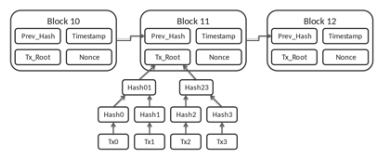
\includegraphics[width = .7\textwidth]{images/lezione6/approccio.png}
\end{center}
In una blockchain le transazioni sono raggruppate in blocchi (di n numeri di transazioni, dove n può essere diverso da un blocco a un altro) che hanno:
\begin{itemize}
    \item Timestamp di quando il blocco è stato creato
    \item Tx\_Root è una struttura dati (merkle tree: molto efficiente capire se una transazione è contenuta o meno nel blocco) che serve per memorizzare le transazioni che stanno dentro al blocco. Ogni transazione ha un hash che la rappresenta. 
    \item Nonce: un numero
    \item Prev\_Hash: collegamento al blocco precedente tramite il suo hash
\end{itemize}
\textit{Ogni nodo partecipante ha una copia della blockchain intera.}

\subsection{Problemi}
I sistemi di cui stiamo parlando sono asincroni, difficili da gestire a causa di latenza indecidibile, sincronizzazione imprecisa del clock e nodi malevoli, tutte caratteristiche che comportano:
\begin{itemize}
    \item l'ordine di arrivo delle transazioni possono essere diversi su diversi nodi
    \item alcune transazioni potrebbero contraddirsi a vicenda
    \item nodi diversi possono costruire diversi blocchi
    \item nodi diversi possono ritrovarsi con catene diverse (non si ha consenso)
\end{itemize}

\subsection{Consenso nella blockchain}
La sfida è quindi avere per ogni nodo il consenso sui blocchi e sulla sequenza di blocchi (sulla catena).\\
L'idea principale dell'algoritmo è:
\begin{enumerate}
    \item calcoliamo l'hash di ogni transazione e di un blocco
    \item quando calcolo l'hash del blocco inserisco nella funzione di hash anche l'hash del blocco precedente
    \item si include un trucco per rendere la computazione dell'hash del blocco molto dispendiosa(processo di mining), ma molto facilmente verificabile (proof of work)
    \item  se abbiamo un certo numero di nodi che vogliono fare un lavoro li si fanno competere e c'è una ricompensa (valuta di quella blockchain) per il vincitore, che si occuperà di distribuire il blocco calcolato a tutti gli altri nodi (è come eleggere un nodo che impone il suo blocco)
\end{enumerate}
L'hash di un blocco, di fatto, è la sua firma digitale. Modificando qualcosa all'interno della catena, la catena non sarà più valida, poiché occorrerà ri-validare tutti i blocchi che seguono attraverso il mining. \\
Per controllare se gli hash delle catene sono uguali, controllo l'hash dell'ultimo blocco di ciascuna catena: se sono uguali, ho il consenso sulla catena. Se non ho consenso ho il rischio che nodi diversi abbiano catene diverse.\\\\
Perchè viene dato un lavoro difficile al miner? \\
Perchè ci vorrà del tempo per risolverlo e quindi sarà più difficile avere soluzioni contemporanee. \\
Questo "puzzle" da risolvere viene calibrato in base alla quantità e alla capacità dei miner. Deve essere un problema risolvibile con algoritmi che operano con tecniche brute force, che si può far diventare più difficile progressivamente e che abbia una certa varianza.\\
Ma qual è questo problema così difficile da risolvere?

\subsection{Hashing}
Abbiamo una funzione di hash crittografica f (SHA-256):
\begin{itemize}
    \item dove f(A) ha una lunghezza fissa (per esempio 256 bit, indipendentemente dalla lunghezza dell'input A)
    \item che è resistente alle collisioni (se A diverso B anche f(A) diverso f(B)) 
    \item dove è molto difficile trovare A a partire da f(A)
    \item dove è molto facile calcolare f(A), cioè è facile verificare dati A e B se B = f(A)
\end{itemize}


\subsection{Algoritmo PoW nella Blockchain}
Il compito del miner è trovare il Nonce tale per cui il valore dell'hash finale sia più piccolo di un certo numero, scelto in modo collettivo, affinchè il tempo di risoluzione rimanga costante nel tempo.\\
Il computer deve provare con un meccanismo di brute force tutti i Nonce fino a quando non trova quello che soddisfa i requisiti.\\
È un problema progettato per richiedere un certo lasso di tempo, in modo da diminuire al minimo la probabilità che due miner risolvano l'enigma nello stesso momento.\\
Quando un miner risolve il puzzle lo annuncia a tutti.\\
Gli altri nodi, quando ricevono un messaggio da un nodo che dice di aver risolto un blocco, se effettivamente è stato verificato, lo aggiungono alla copia locale della loro catena. \\
\begin{center}
    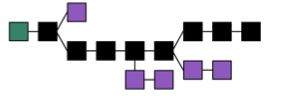
\includegraphics[width = .6\textwidth]{images/lezione6/chain.png}
\end{center}
La catena può avere dei branch (come possiamo vedere anche dalla foto), poiché siamo in una modalità concorrente, cioè i processi vengono eseguiti su nodi diversi ed è difficile prevedere chi finisce prima o dopo o quasi nello stesso momento. \\
È possibile che arrivino due blocchi entrambi validati e che abbiano lo stesso indirizzo del blocco precedente, nonostante siano diversi, formando quindi un branch.\\
La proprietà del Proof of Work fa si che ci sia una catena che si sviluppa più velocemente delle altre e che è quindi la porta ad essere la principale. \\
I blocchi che rimangono pendenti e che non fanno parte della catena prevalente, devono essere svuotati delle loro transazioni, che vengono rimesse nella pool di transazioni pending, a meno che non facciamo già parte di un blocco nella catena principale. \\
Saranno poi pescate in successivi tentativi di composizione dei blocchi.
(?) Un miner prende delle transazioni dal pool del pending, senza nessuna politica di selezione. Diversi miner possono prendere diverse transazioni. Se due miner sono al corrente di uno stesso blocco e sono d'accordo su di questo, prendono due insieme di transazioni diverse, lo risolvono e quando lo restituiscono al nodo vengono aggiunti entrambi generando il branch.(?)

\subsection{Proprietà della blockchain}
\begin{itemize}
    \item Assumendo che il maggior numero dei nodi stanno lavorando sulla stessa catena, quella che cresce più velocemente sarà la più lunga e la più veritiera.
    \item Un nodo malevolo se vuole modificare la transazione di un nodo intermedio deve anche ri-minare tutti i blocchi successivi e deve anche prevalere su tutti gli altri nodi della rete.
    \item Il meccanismo della blockchain è sicuro finchè più del 50\% del lavoro dei miner è onesto
\end{itemize}

\subsection{Limiti del Proof of Woork}
Ci sono tantissime critiche a questo algoritmo di consenso, per cui sono emerse altre proposte. \\
Non è il PoW che fa funzionare la blockchain, è l'algoritmo di consenso in generale ad essere importante.\\
I principali difetti sono:
\begin{itemize}
    \item consumo di energia e risorse (circa 1 miliardo di euro al giorno)
    \item numero di transazioni al secondo limitate
\end{itemize}

\subsection{Proof of Stake}
È detto proof-of-stake (PoS, vagamente traducibile in italiano come "prova che si ha un interesse in gioco") un tipo di protocollo per la messa in sicurezza di una rete di criptovaluta e per il conseguimento di un consenso distribuito. È basato sul principio che a ogni utente venga richiesto di dimostrare il possesso di un certo ammontare di criptovaluta. Si differenzia dai sistemi proof-of-work che sono basati su algoritmi di hash che validano le transazioni elettroniche. Peercoin è stata la prima criptovaluta ad introdurre sin dal lancio il sistema Proof of Stake senza mai implementarlo completamente. Altre note implementazioni del PoS sono BitShares, Nxt, BlackCoin e Cardano.

\subsubsection{Varianti per la selezione di un blocco}
Ogni qualvolta un nuovo blocco viene aggiunto alla blockchain, deve essere scelto il creatore del blocco successivo. Dato che quest'ultimo non può essere l'account che possiede la maggiore quantità della criptovaluta (altrimenti questo creerebbe tutti i blocchi), sono stati escogitati diversi metodi di selezione.


\paragraph{Selezione casuale (random)}
Nxt e BlackCoin utilizzano una funzione casuale per predire il generatore del blocco successivo, impiegando una formula che cerca il valore hash più basso rapportato alla dimensione della somma in gioco. Dato che la conoscenza delle somme è pubblica, ogni nodo della rete può predire - con ragionevole accuratezza - quale account si aggiudicherà il diritto di forgiare un nuovo blocco.

\paragraph{Selezione basata sull'anzianità}
La PoS di Peercoin mescola la selezione casuale con il concetto di "anzianità", un numero ottenuto tramite il prodotto del numero di monete per il numero di giorni in cui tali monete sono state possedute. Le monete che non sono state spese per almeno 30 giorni competono per la creazione del blocco successivo. Gli ammontari di monete più anziani e più grandi hanno una maggiore probabilità di firmare il blocco successivo. Eppure quando un ammontare di monete è utilizzato per firmare un blocco, questo ammontare deve ricominciare con "anzianità zero" e quindi aspettare almeno altri 30 giorni prima di poter firmare un altro blocco. E inoltre la probabilità di trovare il blocco successivo è massima dopo 90 giorni, per prevenire che somme consistenti e molto "anziane" possano dominare la blockchain. Questo processo mette in sicurezza la rete e produce gradualmente nuova valuta nel corso del tempo senza consumare una potenza computazionale significativa. Gli sviluppatori di Peercoin sostengono che questo renda più difficile attaccare la rete dato che cade il bisogno di piattaforme centralizzate di mining e inoltre acquistare più di metà delle monete è probabilmente più costoso che acquisire il 51\% della potenza di hashing della proof-of-work.

\paragraph{Selezione basata sulla velocità}
Il concetto di PoS di Reddcoin basata sulla velocità rivendica di incoraggiare la movimentazione di moneta piuttosto che il suo accumulo.

\paragraph{Selezione basata sul voto}
Invece di utilizzare solamente il concetto di posta in gioco (stake), i creatori dei blocchi possono essere selezionati mediante votazione. BitShares utilizza un sistema che comprende 101 delegati e sceglie casualmente tra essi.[1] Il voto della comunità aumenta l'incentivo dei creatori dei blocchi ad agire responsabilmente, ma al contempo apre alla prospettiva di scenari di sybil attack - come ad esempio nell'eventualità che un singolo utente impersoni i primi cinque delegati.

\subsection{Raft}
Raft è algoritmo per il consenso che è stato progettato per essere facile da capire. È l'equivante a Paxos a livello di fault-tolerance e performance.\\
Questo protocollo scompone il codice in sottoproblemi relativamente indipendenti tra loro e affronta ogni “pezzo” singolarmente.\\
Lo scopo principale di Raft è quello di rendere il consenso disponibile ad un pubblico sempre più vasto e che quest’ultimo sarà in grado di sviluppare nuovi sistemi basati sul consenso.\\
Raft si occupa della replica dei log. Intuitivamente, se si riesce a far apparire la stessa identica sequenza di log sulla maggior parte delle macchine, si è riusciti a far sì che quel cluster di macchine concordi su qualcosa.\\
In effetti, questo è chiamato trasmissione dell'ordine totale.\\ Se si riesce a far apparire ogni voce del log nella stessa posizione in un cluster di macchine, si può usarlo per implementare il consenso. \\
Ad esempio, se una macchina vuole proporre un valore e supponiamo che la sua ultima voce di registro sia nella posizione i, può provare a far sì che altre macchine mettano questo nuovo valore in i + 1 . Dopo che la maggior parte delle macchine nel cluster ha replicato quel valore in i + 1 , ora chiamiamo quel valore impegnato in i + 1 . Questo è effettivamente lo stesso che proporre un valore e farlo accettare da altri nei termini di Paxos.\\
Raft è un protocollo basato su leader. Nel suo normale corso operativo, un solo leader sarà eletto dal cluster di nodi. Gli altri nodi sono seguaci. Il leader accetta le richieste di scrittura del cliente e le replica ai follower.\\
Se si vogliono avere informazioni più approfondite su Raft si può leggere
\href{https://ichi.pro/it/protocollo-raft-consensus-reso-piu-semplice-160718622511489}{questo articolo} che ne spiega in dettaglio il funzionamento.


\subsection{Smart Contracts}
La blockchain è utile per salvare cose che vanno oltre a transazioni finanziarie. Ad esempio Ethereum è stata progettata per gli smart contracts.\\
Gli smart contract sono porzioni di codice software definiti come contratti self-executing.\\Sebbene originariamente sono stati proposti come versione digitale di contratti legali, possono essere dei programmi software generali.\\
Ogni contratto è salvato nella blockchain, diventando così immutabile.\\
Ogni nodo può verificare se le condizioni del contratto sono soddisfatte e eseguire determinate azioni (l'output deve essere validato in maniera distribuita). Alla fine tutti i nodi devono essere d'accordo sullo "stato" risultante.\\
Un esempio di applicazione potrebbe essere una piattaforma di crowdfounding senza autorità centrale.

\subsection{Permissionless vs Permissioned DLT}
Le blockchain di Bitcoin ed Ethereum sono chiamate permissionless poichè:
\begin{itemize}
    \item si ha un DL decentralizzato che traccia tutte le transazioni
    \item non ci sono terze parti fidate
    \item si ha accesso incondizionato al ledger
    \item si ha la validazione delle transazioni e la generazione di nuove monete da parte dei miners
    \item si ha la pseudo-anonimità dei partecipanti
    \item le transazioni sono immutabili
\end{itemize}
Esistono anche DLT permissioned, che vengono sfruttate soprattutto in ambito business dove ci sono molte istituzioni che usano questo meccanismo in un insieme trust limitato.\\
In queste DLT:
\begin{itemize}
    \item si ha un DL decentralizzato che traccia tutte le transazioni
    \item ci sono una o più terze parti fidate
    \item si ha un accesso condizionato al ledger
    \item  si ha la validazione delle transazioni e la generazione di nuove monete da parte dei miners
    \item si conosce l'identità dei partecipanti
    \item le transazioni sono immutabili
\end{itemize}

\subsubsection{Hyperledger Fabric}
Hyperledger nasce nel 2015 come consorzio di industrie che ha lo scopo di sviluppare una blockchain open-source per il business, hostata da Linux Foundation.\\
Fabric è uno dei sottoprogetti, originariamente gestito da IBM) che prevedeva:
\begin{itemize}
    \item permissioned DLT
    \item architettura modulare in grado di adattarsi a diversi requisiti: transazioni private, contratti confidenziali, diversi protocolli di consenso
    \item app (contratti) distribuite in linguaggi di programmazione generici
    \item nessuna dipendenza da criptovalute native
\end{itemize}



\begin{comment}
ociredeF


==============

ramO

Il problema del consenso è uno dei problemi fondamentali nel blockchain.
Nell'ambito business è considerata una tecnologia essenziale.
Nasce dalla nascita di bitcoin in avanti. Gli algoritmi che stanno alla base del paper che ha introdotto il bitcoin sono antecedenti. Il creatore di bitcoin lo ha ideato prendendo sputo da ricerca nei sistemi distribuiti. Questo whitepaper apparso nel 2008 è stato rivoluzionario. Firmato da uno pseudonimo, di cui ancora oggi non sappiamo il nome. 
Bitcoin: p2p cash system
Un mese prima dall'uscita del paper qualcuno ha registrato il nome Bitcoin, intuendo che avrebbe potuto rivoluzionre l'ambito finanziario.
Nel 2009 esce una prima implementazione di questo sistema open source. Da lì varie altre implementazioni e varianti. Questo meccanismo non va bene solo per denaro elettronico, ma ha potenziai applicazioni in molti altri ambiti. Potrebbe addirittura essere la base per avere applicazioni trusted distribuite, il cui output è trusted nonostante possano essere eseguite anche da nodi malevoli.

Nel 2013 nasce Ethereum e poi tante altre DLT.

La caratteristica di blockchain è che implementa un specie di registro delle cose che avvengono (ad esempio il registro delle transazioni immobiliari/catasto) che è immutabile (si può osservare tutta la storia). La novità è la distribuzione, non c'è un "catasto"/database(?) centralizzato che memorizza i dati, bensì è distribuito. L'obbiettivo è rendere storica l'informazione, immutabile (posso solo aggiungere e non posso cancellare), distribuita e fault tolerant (non soltanto crash, ma anche bizantine, poiché non ho fiducia in alcuni nodi che partecipano).

Le applicazioni della blockchain sono ampie. Dai quadri ai videogiochi, etc.

Il DLT System Model è un sistema distribuito. Ha un controllo decentralizzato, in cui ogni nodo esegue lo stesso codice e non c'è un controllore vero e proprio. Questi nodi sono gestiti da entità separate, non c'è un comune amministratore, e non si fidano gli uni degli altri (anche se ci sono DLT con assunzioni di trust). Dunque questo distribuito ha potenzialmente nodi con comportamento bizantino. Mettiamo una copia di tutto dappertutto. Tutti hanno una copia di questo "catasto".
Il problema del consenso, in questo caso, è che i nodi devono essere d'accordo, non sull'ultimo dato memorizzato, bensì sulla storia dei dati. 
Una blockchain è una sequenza storica di transazioni. Una transazione è un record di dati (in generale, dopodiché, essendo stata proposta in ambito finanziario ...).
Una transazione per convenzione deve avere stesso input e stesso output. Non si memorizza mai il saldo, bensì le entrate (?).

Ogni transazione che viene inserita viene firmata. Questa transazione firmata viene mandata a tutti i nodi della blockchain, perché la stessa informazione deve essere memorizzata da tutti. Nella blockchain si è identificati dalla coppia chiave pubblica/privata (se ne possono avere molte e quindi identità blockchain diverse). Quando un nodo riceve una transazione sa che arriva da un certo indirizzo blockchain. Nella transazione c'è anche la ciave pubblica del mittente in modo da fare verifiche ulteriori. C'è quindi un meccanismo di crittografia che garantisce l'origine.
Quando un nodo riceve la transazione, la valida. Come questo avviene fatto dipende dal tipo di applicazione. Bitcoin controlla dallo storico se aveva soldi dallo storico (?). Dopodiché la mette in un pool di transazioni pending. 
Da questo insieme di transazioni pending, si raggruppano in un blocco (non tutti i blocchi hanno stesso numero di transazioni). Questo blocco ha un timestamp (non necessariamente lo stesso di tutte le transazioni che sono dentro). Timestamp di quando ho fatto il blocco, non di quando ciascuna transazione è stata inserita.
ESEMPIO
Il blocco 11 contiene 4 tranazioni. Sono alla base dell'albero da Tx0 a Tx3. Sono organizzate in una struttura dati Merkle Tree, una struttura dati particolarmente efficiente per una determinata operazione. Queste transazioni hanno un corrispondente valore di hash. Abbiamo quindi una funzione di hash. Questa struttura dati è molto efficiente per capire se una transazione è contenuta oppure no nel blocco guardando l'hashing della radice. C'è inoltre un timestamp, un numero (nonce) e un "puntatore" contente un valore digitale che rappresenta il blocco precedente della catena. La cosa importante è che ognugno dei nodi ha un copia di questa blockchain. 
Blocchi e tranaszioni potrebbero avere timestamp diversi in diversi nodi, non avendo sincronizzazione perfetta. 
I problemi sono dovuti al fatto che i sistemi di cui stiamo parlando sono sistemi asincroni. Si possono fare assunzioni e accettare che qualcosa vada male, controllando poi che cosa va male. 
Problemi che in alcuni casi sono impossibili da risolvere in modo perfetto.
- La propagazione non arriva nello stesso ordine a tutti. 
- Transazioni possono essere contraddittorie
- Se le transazioni pending vengono accumulate da ogni nodo, posso avere che due nodi fanno blocchi diversi contemporaneamente.
- Possono avere catene diverse. Tutti devono avere stessa catena (problema del consenso).

L'idea dell'algoritmo proof of work è:
- calcoliamo l'hash di ciascun transazione, che da un valore come output che rappresenta quell'oggetto
- calcolo l'hash del blocco, inserendo nella funzione di hash del blocco l'identità del blocco precedente nella catena
- I nodi che calcolano l'ash del blocco devono fare un lavoro significativo (non tutti i nodi della blockchain lo fanno) chiamato mining. Alcuni dei nodi si rendono volontari di fare questo lavoro di calcolare l'hash secondo un certo trucco che è stato inserito. Chi guarda il lavoro fatto, immediatamente capisce se è fatto bene o male. Costoso da svolgere, ma immediatamente verificabile.
- Se abbiamo un certo numero di nodi (miner) che vogliono fare il lavoro, li facciamo competere. C'è un ricompensa in termini di valuta della blockchain. Si vuole eleggere quello che risolve per primo l'enigma matematico. Ci vuole anche un meccanismo per far sì che sia imrobabile (ma non impossibile) che due risolvano il problema nello stesso istante.
Diamo a ciascun miner un compito difficile in modo che ci debba mettere del tempo e sia molto improbabile che lo risolvano nello stesso momento. Questo puzzle viene calibrato man mano che i miner aumentano la capacità di risolvere il problema. 
Deve essere un problema risolvibile con brute force, che posso far diventare più difficile progressivamente e che abbia una certa varianza.

Abbiamo una funzione di hash crittografica (es. SHA256). Voglio che il suo output non sia dipendente dall'input in termini della lunghezza della stringa. Sempre stessa lunghezza. Se lo applico a due input diversi, l'output deve essere diverso. Deve essere molto difficile ricostruire input da output. Deve essere anche molto veloce calcolare l'hash e posso verificare facilmente che dato l'input A e l'output B, B = f(A).

Demo blockchain:
Il mining consiste nel trovare un nonce tale per cui l'hash del blocco sia più piccolo di un certo numero, scelto in modo collettivo affinché il tempo di risoluzione rimanga costante nel tempo. All'interno della blockchain, ogni blocco contiene l'hash del blocco precedente. L'hash di un blocco, di fatto, è la sua firma digitale. Modificando qualcosa all'interno della catena, la catena non sarà più valida, poiché occorrerà ri-validare tutti i blocchi che seguono attraverso il mining. Per controllare se gli hash delle catene sono uguali, controllo l'hash dell'ultimo blocco di ciascuna catena. Se sono uguali, ho il consenso sulla catena. Se non ho consenso, ho il rischio che nodi diversi abbiano catene diverse (?).

Il numero di transazioni può essere diverso nei diversi blocchi.

I messaggi sono firmati, per cui diventa più semplice risolvere il problema di consenso bizantino. Devo avere almeno la maggioranza dei nodi che non hanno il comportamento bizantino (2k + 1) per falsificare la transazione (?).

Risultato rilevante è il trucchetto della PoW. Quando un miner risolve il puzzle, lo annuncia a tutti. Gli altri nodi, quando ricevono un messaggio che dice di aver risolto un blocco (viene quindi mandato blocco e hash che dimostra la risoluzione facilmente verificabile), se effettivamente è stato verificato, lo aggiunge alla copia locale della catena. La catena può avere dei branch, poiché siamo in una modalità concorrente, cioè i processi vengono eseguiti su nodi diversi ed è difficile prevedere chi finisce prima o dopo o quasi nello stesso momento. è possibile che arrivino due blocchi entrambi validati e che abbiano lo stesso indirizzo del blocco precedente, nonostante siano diversi, formando quindi un branch. La proprietà del PoW fa si che ci sia una catena che si sviluppa più velocemente delle altre e che è quindi quella condivisa da tutti. I blocchi che rimangono pendenti e che non fanno parte della catena prevalente, deve rimettere le transazioni che erano in questo blocco nella pool di pending, a meno che non facciamo già parte di un blocco nella catena. Saranno pescate in successivi tentativi di composizione dei blocchi.

Un miner prende delle transazioni dal pool del pending, però non c'è una politica di selezione. Diversi miner possono prendere diverse transazioni. Se due miner sono al corrente di uno stesso blocco e sono d'accordo su di questo, prendono due insieme di transazioni diverse, lo risolvono e quando lo restituiscono al nodo vengono aggiunti entrambi generando il branch.

I miner sono anche nodi della catena.

Le proprietà che emergono sono:
- se la maggior parte dei nodi lavorano sulla stessa catena ...
- non solo, se vuole cambiare qualcosa nella catena, deve ricalcolare i blocchi, ma deve anche imporsi sulla catena più lunga (?).
- più del 50\% del lavoro dei miner deve essere onesto

Ci sono tantissime critiche a questo algoritmo di consenso, per cui sono emerse altre proposte. Non è il PoW che fa funzionare la blockchain, è l'algoritmo di consenso in generale ad essere importante.

L'elettricità costa parecchio per fare PoW (1 miliardo al giorno) e le transazioni sono poche.

Il consenso non c'è mai sull'ultimo blocco soltanto, ma dev'essere sulla storia della catena.

Sono stati proposti diversi algoritmi di consenso, ad esempio Raft, algoritmo di consenso per altro tipo di blockchain: permissioned (?).
Proof of stake sostiene che chi ha più potere/risorse decide quale blocco aggiungere. In più c'è un meccanismo randomico, non c'è la selezione esatta di chi ha più risorse. Inoltre c'è il discorso dell'età: da quanto tempo questo verificatore del blocco fa parte della blockchain? Più è alto è il tempo, più è alta la fiducia. L'intuizione dietro a questa scelta è che il danno che loro avrebbero nell'essere malevoli nella blockchain è superiore al guadagno. Quando uno di questi volontari viene scelto, il suo account viene congelato fino a quando non si capisce che la validazione è stata corretta e dopodiché viene rilasciato.

In Raft viene fatta un'elezione in modo distribuito. Non sempre è l'id maggiore che vince, poiché questo può essere costruito per esempio guardando quanti soldi hanno nel conto e far emergere quello che ha più soldi. Bisogna escludere quello dal comportamento malevolo, poiché si è deciso di farlo in termini di fiducia. Se il validatore cerca di compromettere il sistema/validare transazioni fraudolenti dentro al blocco, perdono tutto.

Come si previene il double spending problem? (uso i miei soldi per due transazioni cercando di comprare due cose con gli stessi soldi)
VIDEO

Nel 2012-13 è apparso un articolo che propone una generalizzazione dell'uso di blockchain, rendendo esplicita la cosa. Da qui nasce Ethereum, che generalizza, rispetto a transazioni finanziarie, a smart contract (più eterogenea) e ha un suo linguaggio per scrivere gli smart contract.

Queste blockchain vengono chiamate permissionless: chiunque può decidere di partecipare e vedere le transazioni dentro la blockchain. C'è pseudoanonimità dei partecipanti. 

Ci sono anche DLT permissioned. Soprattutto in ambito business ci sono molte istituzioni che usano questo meccanismo tra un insieme di aziende (trust limitato). Limitare la partecipazione e aggiungere un controllo. Abbiamo identità nota dei partecipati. Ci sono delle identità trusted. Ci sono anche qui criptovalute legate a questo. Una di queste piattaforme per la generazione di DLT è hyperledger, in particolare hyperledger fabric (inizialmente fatto da IBM e poi ceduto). È possibile sviluppare gli smart contract (in ethereum c'è un linguaggio apposta) con general purpose programming languages, posso quindi scrivere codice all'interno dei dati che vengono racchiusi in blocchi.

------------
Fabbio
DLT: tecnologie blockchain

Nell'ambito business la blockchain è considerata una tecnologia essenziale. 
Storia:
Nel 2008 nasce un paper firmato da satoshi nakamoto (pseudonimo) intitolato Bitcoin. Bitcoin è un peer-to-peer cash system. Il mese prima dall'uscita del paper qualcuno aveva registrato il nome Bitcoin.
Nel 2009 esce la prima implementazione opensource e da lì in poi varie implementazioni e varianti.
Il meccanismo ha potenziali applicazioni in moltissimi ambiti. Potrebbe essere la base per avere applicazioni distribuite trusted il cui output è trusted nonostante possano essere eseguite anche da nodi malevoli.

nel 2013 esce ETH e via...

La caratteristica di blockchain che ispira altre applicazioni oltre al denaro elettronico è che implementa un registro delle cose che avvengono (tipo registro transazioni immobiliari o catasto immobiliare..). 
A differenza dei database il "catasto" viene distribuito su vari nodi. L'obiettivo è rendere storica, immutabile e full tolerance l'informazione.


Il modello del sistema DLT
-E' un sistema distribuito
-Ha un controllo decentralizzato in cui non c'è un coordinatore e ogni nodo esegue lo stesso codice
-I nodi sono gestiti da entità separate e non si fidano gli uni degli altri
Dunque il sistema distribuito ha assumibilmente nodi con comportamento "bizzantino"

Problema del consenso:
I nodi devono essere d'accordo su di uno storico dei dati. I nodi devono essere d'accordo sulla storia dei dati.

DATI NELLA BLOCKCHAIN
Una blockchain è una sequenza storica di transazioni
Transazione: Record di dati. Nell'ambito finanziario [A trasferisce x a B]
Una transazione per convenzione deve avere lo stesso input e lo stesso output.

L'APPROCCIO BLOCKCHAIN
Ogni transazione inserita viene firmata. Si utilizza il meccanismo di chiavi asimmetriche e ogni partecipante ha una chiave privata e una pubblica. Quando una transazione viene firmata, questa viene mandata a tutti i nodi della blockchain.
Quando un nodo riceve una transazione sa da quale nodo arriva. 
Nel codice condiviso che tutti i nodi hanno, c'è una porzione che dice "Quando arriva una transazione validala". Dunque il nodo che riceve va a vedere nello storico se la transazione è plausibile. 
Dunque: A mette una tranazione nel sistema che va a tutti i nodi. Chi la riceve guarda nello storico se è valida. Poi la mette in un pool di transazioni pending.
QUANDO PASSA IN UNO STATO APPROVED?

APPROCCIO BLOCKCHAIN:
Dall'insieme di transazioni pending, si raggruppano in un blocco (non tutti i blocchi hanno lo stesso numero di transazioni), il blocco ha un timestamp che non è lo stesso di tutte le transazioni che ha al suo interno. Nel blocco X (11 nelle slide) c'è il TX room: struttura dati per memorizzare le transazioni nel blocco. Ogni transazione ha il corrispondente valore di hash e la struttura dati ha la particolarità che è molto efficiente capire se una transazione è avvenuta o no.
C'è un certro numero di transazioni nel blocco e c'è una funzione per capire molto velocemente se all'interno del blocco c'è o meno la transazioni.
Da un blocco all'altro si collegano tramite un puntatore (valore digitale del blocco precedente viene scritto nel blocco successivo e viceversa). 
Ognuno dei nodi ha la copia di questa blockchain.

PROBLEMI:
I blocchi e le transazioni potrebbero avere timestamp diversi su diversi nodi. 
I problemi sono dovuti al fatto che i sistemi sono asincroni dove possono capitare le cose più bizzarre. Alcune transazioni potrebbero essere contraddittorie. Nodi diversi potrebbero creare blocchi diversi. Tutti i nodi devono avere la stessa blockchain. (Problema del consenso)

CONSENSO DELLA BLOCKCHAIN
Idea: si calcola l'hash di ogni transazione che da in output un certo valore che rappresenta l'oggetto. Calcolo l'hash del blocco. Quando calcolo l'hash del blocco inserisco l'identità digitale del blocco precedente e ci includo...
Non tutti i nodi della blockchain fanno il lavoro del calcolo dell'hash, e questo lavoro viene fatto dai miners. I miners introducono nella blockchain nuova valuta.
Alcuni dei nodi dunque si rendono volontari per calcolare l'hash con un trucco particolare. Il lavoro è duro e costoso ma immediatamente verificabile. (Idea dietro l'algoritmo di consenso)
Se si hanno un certo numero di nodi che vogliono minare, li si fa competere su di un blocco. C'è un compenso nella valuta della blockchain. Diversi nodi dunque si mettono a validare un blocco è tra tutti questi bisogna sceglierne uno. Quello che si elegge è quello che risolve prima "l'enigma matematico". Ci può essere il caso in cui 2 riescono risolvere il puzzle allo stesso momento.

PROBLEMI DIFFICILI:
perchè deve essere difficile? Perchè devono metterci tempo così che tutti finiscano in tempi differenti. La difficoltà del puzzle viene aumentata in base alla capacità del miner di risolvere il problema. Il problema deve essere un problema che dal punto di vista computazionale viene risolto in bruteforce, può avere una certa varianza (puoi essere fortunato o sfortunato a risolverlo).
Statisticamente è più difficile che più miners lo risolvono a diversi istanti.

QUAL è QUESTO PROBLEMA?
Funzione di Hashing crittografica con proprietà tipo:
Output indipendente dalla lunghezza dell'input.
Deve essere collision resistent.
Dallì'output deve essere quasi impossibile risalire all'input.
Deve essere facile da verificare.

PROPRIETA' BLOCKCHAIN:
La catena che cresce più velocemente sarà quella che merita fiducia. 


\end{comment}

%\chapter{}
\chapter{Augmented Reality in pratica}
\lhead{Augmented Reality in pratica - MobiDEV}
\rhead{Lezione 7 - 25 marzo}
\begin{center}
    \textbf{--------- Lezione 7 - 25 marzo 2021 ---------}
\end{center}

\section{Panoramica}
Le due librerie principali per lo sviluppo di applicazioni AR sono:
\begin{itemize}
    \item ARKit di Apple: è utilizzabile sui device mobili Apple recenti e non utilizzabile su simulatore
    \item ARCore di Google: può essere utilizzata in nativo su Android ed è utilizzabile, con alcune limitazioni, su simulatore
\end{itemize}
\subsection{Macro funzionalità}
Per realizzare applicazioni in realtà aumentata, ARKit e ARCore forniscono funzionalità per semplificare le seguenti operazioni:
\begin{itemize}
    \item Registration e Tracking
    \item Scene
    \item Display
    \item Interaction
\end{itemize}

ARKit e ARCore condividono alcuni concetti base:
\begin{itemize}
    \item scene (ARKit) / session (ARCore): due nomi diversi per lo stesso concetto, che rappresenta l'ambiente rispetto al quale effettuiamo la registration. Gli oggetti virtuali e reali sono posizionati nel sistema di riferimento della scena/sessione. Fornisce le chiamate per accedere agli altri elementi di AR
    \item configuration: definisce le caratteristiche della scena / sessione da creare:
    \begin{itemize}
        \item rispetto a cosa facciamo la registration, ad esempio rispetto all'ambiente 3D circostante, viene creato un sistema di riferimento in una posizione iniziale e si tiene traccia dello spostamento rispetto a questo sistema
        \item rispetto a cosa siamo interessati a riconoscere
    \end{itemize}
    \item ancore: rappresentano dei punti di riferimento agli oggetti virtuali o reali identificati. Es: quando un oggetto viene riconosciuto, viene associato ad un’ancora. Attraverso l’ancora possiamo risalire alla posizione e rotazione (6DOF) dell'oggetto rispetto alla scena. Le ancore si usano ad esempio quando riconosciamo i piani ed ogni piano è rappresentato dalla propria ancora
    \item hitTest/rayCasting: si tratta di un’operazione per convertire le coordinate schermo (2D) in un punto 3D. Concettualmente devo considerare il raggio, che “esce” dal device verso lo spazio, che interseca zero o più oggetti (reali o virtuali) ed hitTest ritorna l’insieme di questi oggetti
\end{itemize} 

\subsection{Comprendere la scena}
ARKit e ARCore forniscono alcuni strumenti che semplificano il processo di comprensione della scena:
\begin{itemize}
    \item riconoscimento piani
    \item riconoscimento immagini (2D): la procedura avviene in 3 passi:
        \begin{itemize}
            \item aggiunta dell'immagine alle risorse del progetto: si fornisce ad ARKit/ARCore l'immagine da riconoscere e la dimensione attesa nel mondo reale
            \item modifica della configurazione della scena, indicando, da codice, che si vuole riconoscere quell'immagine
            \item specificare cosa fare quando l'immagine viene riconosciuta: si gestisce l'evento di quando l'ancora relativa a quell'immagine viene aggiunta
        \end{itemize}
    \item riconoscimento dei volti
    \item riconoscimento oggetti (3D): dobbiamo prima ottenere un modello 3D dell'oggetto e poi il procedimento di riconoscimento è analogo a quanto avviene per le immagini 2D 
\end{itemize}

\section{Alcune funzionalità di ARKit 4}
\subsection{AR multiuser}
Sia in ARKit che in ARCore si possono avere più scene/sessioni condivise tra più utenti. 
Prendiamo ad esempio un utente identifica dei feature point e poi si identifica tramite l'ambiente. Se quelle stesse informazioni vengono condivise con un altro utente e il device di questo, riesce a capire dove si trova rispetto ai fp del primo utente, possiamo fare la registrazione rispetto ad un sistema di riferimento comune. Questo permette di mostrare un oggetto virtuale nello stesso punto a diversi utenti con diverse angolazioni. 
\begin{center}
    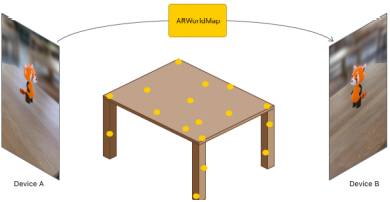
\includegraphics[width=.7\textwidth]{images/MobiDEV/5. augmented reality in pratica/ar multiuser.PNG}
\end{center}

\subsection{Scene geometry}
I device che hanno un sensore di profondità (Lidar) possono creare una ricostruzione topologica dell'ambiente. La libreria AR per i dispositivi con Lidar mette a disposizione funzionalità per:
\begin{itemize}
    \item riconoscere gli oggetti
    \item calcolare quando un oggetto si interpone tra la camera e un oggetto virtuale, così da risolvere il problema dell'occlusione
    \item permettere agli oggetti virtuali di rispettare alcune regole della fisica nell'interazione con oggetti del mondo reale (ad esempio due oggetti che non si possono compenetrare)
\end{itemize} 
Attraverso il lidar è anche possibile andare a creare una configurazione chiamata body tracking dove il sistema riconosce le principali articolazioni del corpo e ce le restituisce come nodi, ovvero punti che possiamo tracciare, cosicché possiamo calcolare la posizione del corpo e come si muove l'utente. Questa procedura si chiama \textbf{Motion capture}.

\chapter[Activity recognition - Gabriele Civitarese]{Activity recognition - Gabriele \\Civitarese}
\lhead{Activity recognition (Gabriele Civitarese) - MobiDEV}
\rhead{Lezione 8 - 8 aprile}
\begin{center}
    \textbf{--------- Lezione 8 - 21 ottobre 2020 ---------}
\end{center}

\section{Approccio alla scrittura del codice}
La scrittura di un programma di un sistema complesso passa attraverso una serie di errori. 

Uno degli errori più comuni è scrivere tutto o buona parte del codice e poi verificare se l'effetto finale del software realizzato è quello desiderato. 
Il problema è che non funziona mai al primo tentativo e correggere gli errori diventa molto complicato, perché non si sa dove possono essere.

L'idea è quella dividere il processo di sviluppo in tanti piccoli passi, ognuno dei quali può essere provato per controllarne il funzionamento. 
Più difficile è il codice che si scrive, più i passi devono essere piccoli. Anche una sola riga di codice, se ad esempio si sta usando una tecnologia che non si conosce bene. 

Il problema è che, a volte, abbiamo delle righe di codice che non producono un effetto visibile, come la gestione degli eventi. 
Per questo bisogna scrivere del codice per verificare lo stato di un'applicazione, come l'utilizzo di messaggi di log.

Il tempo di sviluppo è in buona parte dedicato a correggere gli errori soprattutto quando lo sviluppatore è inesperto che scrive tutto il codice insieme. 
Ridurre il numero di errori e il tempo necessario per correggerli è 
l’obiettivo principale se si vuole sviluppare velocemente.

Dividere il codice in piccole parti verificabili è difficile. 
Prima di iniziare a sviluppare una parte di codice bisogna pensare a come suddividerla in parti, sfruttando l'utilizzo di carta e penna, o di algoritmi in pseudo codice. 
Un errore comune è che viene provata l'app senza sapere cosa aspettarsi. Prima di fare una prova bisogna pensare a cosa ci si aspetta che sia il risultato.

Diverse parti del codice vengono adattate da esempi trovati online. Questi sono i casi nei quali è più facile commettere errori, perché magari non conosciamo esattamente le operazioni che fa il codice. 

Due strategie di sviluppo sono:
\begin{itemize}
    \item top-down: iniziare a scrivere le funzioni principali per poi scrivere i metodi di dettaglio che sono necessari per le funzioni principali
    \item bottom-up: iniziare a scrivere i metodi di dettaglio per poi comporli nelle funzioni principali
\end{itemize}

Prendiamo ad esempio un algoritmo di ordinamento di un array composto da due funzioni:
\begin{itemize}
    \item la funzione principale di ordinamento
    \item la funzione che scambia il valore di due elementi dell'array
\end{itemize}
Nell'approccio top-down prima viene scritta la funzione principale di ordinamento, poi quella che scambia i due valori

Nell'approccio bottom-up prima viene scritta la funzione che scambia i due valori, poi quella di ordinamento.

Nella programmazione tipicamente si usa una combinazione di approccio bottom-up e top-down.

%%%%%%%%%%%%% inizio esempio di algoritmo passo passo %%%%%%%%%%%%%
\begin{comment}

\subsection{Esempio: definizione e problema}
Abbiamo un array che contiene tutte le parole scambiate in 10.000 conversazioni su un sistema di chat. Ogni elemento dell'array è una singola parola. 
L'obiettivo è scrivere un metodo per trovare quante volte occorre una data parola. 

\begin{Java}
    //codice
    ArrayList<String> = wordsArray = ...
    //altro codice
    int a = wordCount(wordsArray, "ciao"); 
    //stampa del valore di a
\end{Java}
\newpage
La prima operazione è quella di ideare la procedura e scrivere il procedimento che risolve il problema: \\
input: array di parole e una parola \\
Output: il numero di volte che la \\
parola occorre nell’array \\
Procedura: \\
- Inizializzo un contatore a zero \\
- Scorro tutte le parole \\
dell'array \\


Poi possiamo procedere a convertire l'algoritmo in codice passo dopo passo:
\begin{itemize}
    \item passo 1: creo un metodo che ritorna sempre lo stesso valore
    \begin{Java}
        private int wordsCount(ArrayList<String> words,
                                String target) {
            return 0;
        }   
    \end{Java}
    \item passo 2: inizializzo e ritorno il contatore
    \begin{Java}
        private int wordsCount(ArrayList<String> words,
                                String target) {
            int counter = 0;
            return counter;
        }   
    \end{Java}
    \item passo 3: verifico di saper scrivere un codice che scorre tutti gli elementi
    \begin{Java}
        private int wordsCount(ArrayList<String> words,
                                String target) {
            int counter = 0;
            for(String word:words){
                counter++;
            }
            return counter;
        }   
    \end{Java}
    \item passo 4: verifico di saper controllare se la prima parola dell’array è quella cercata
    \begin{Java}
        private int wordsCount(ArrayList<String> words,
                                String target) {
            int counter = 0;
            String word = words.get(0);
            if (word.equalsIgnoreCase(target))
                counter++;
            return counter;
        }   
    \end{Java}  
    \item passo 5: metto assieme i due passi precedenti 
    \begin{Java}
        private int wordsCount(ArrayList<String> words,
                                String target) {
            int counter = 0;
            for(String word:words){
                if (word.equalsIgnoreCase(target))
                counter++;
            }
            return counter;
        }   
    \end{Java} 
\end{itemize}
\end{comment}
%%%%%%%%%%%%% fine esempio di algoritmo passo passo %%%%%%%%%%%%%
\section{Testing}
Il testing di un'app ha lo scopo di valutare diversi aspetti:
\begin{itemize}
    \item funzionalità: l'applicazione fa quello che dovrebbe?
    \item usabilità: l'utente riesce ad usare l'app come previsto?
    \item performance: l'applicazione ha le performance desiderate?
    \item sicurezza: l'app è soggetta ad attacchi di sicurezza o privacy?
\end{itemize}

Se emergono problemi durante il testing significa che l'operazione è efficace. 
Se non emergono problemi in fase di test l'applicazione è corretta oppure non sono stati svolti i test corretti. 

Il testing sui dispositivi mobili ha diverse peculiarità: 
\begin{itemize}
    \item i dispositivi sono diversi dal punto di vista hw e sw
    \item diversi contesti di utilizzo: c'è connessione ad internet? potrebbe essere molto rallentata? i server a cui l'app si connette funzionano o sono molto lenti? ecc.
    \item interrupt che avvengono durante l'uso
    \item il codice su dispositivi mobili è basato su eventi. La sequenza con cui avvengono gli eventi spesso non è deterministica e di fatto si pongono dei problemi di concorrenza
\end{itemize}

Il fatto che l’applicazione funzioni una volta non significa che sia corretta perché potrebbe presentare degli errori in futuro, anche se eseguita nello stesso modo sullo stesso HW, SW, nello stesso contesto e con gli stessi interrupt.

Per effettuare un test di un'applicazione concorrente, dobbiamo provare tutte le possibili combinazioni di ordine di chiamate.
Questo però è un problema, perché provare tutte le combinazioni  per ogni device in commercio, è impossibile.

Al posto che svolgere tutti i test per tutti i possibili casi, ciascun test si svolge solo in alcuni caso. In questo modo si hanno meno casi, ma è possibile che qualche caso problematico sia tralasciato. 
\\ Linee guida e best practice da utilizzare:
\begin{itemize}
    \item scegliere i dispositivi più diffusi e caratteristici, tipicamente almeno 2 smartphone e 2 tablet
    \item svolgere i test con la versione minima supportata del SO e uno con la versione più recente
    \item svolgere i test in assenza di problemi e in presenza dei problemi più comuni come la mancanza o il rallentamento della connessione
    \item verificare il funzionamento di tutto il codice
    \item provare l'app su dispositivi diversi
    \item provare l'app in situazioni particolari come assenza o rallentamento della connessione Internet
\end{itemize}

Fare il test di un’applicazione è un’operazione lunga, soggetta ad 
errori che deve essere fatta ogni volta che si mette mano al codice. L'idea è quella di automatizzare il test. 

Alcuni parti possono essere automatizzate, scrivendo del codice che verifica la correttezza di altre parti del codice. 
\\ Questo codice può, ad esempio, creare istanze delle classi del model o generare degli eventi su oggetti di interfaccia. 

Esistono diverse librerie che supportano i test automatizzati. I test automatizzati hanno una chiamata "assert" che indica cosa ci si aspetta sia vero. 
Se tutti gli assert sono verificati, il test ha successo, altrimenti fallisce.
\\ Un esempio ne è il testing del model: viene creata un'istanza della classe che si vuole testare, si richiama il metodo e si verifica, attraverso un assert, che il risultato del metodo sia quello che atteso.
 
Un altro esempio è il testing della view-controller: ci sono librerie che permettono di scrivere del codice al cui interno si possono scatenare degli eventi sugli oggetti interfaccia, ovvero simulare un'azione che farebbe un utente e si verifica che il risultato sia quello atteso.

\subsection{Pro e contro dell'automazione del testing}
Il vantaggio del testing è che dopo aver scritto il codice di test, il test avviene molto velocemente. 
La scrittura di test, però, è onerosa ed è soggetto ad errori: può segnalare errori che non ci sono o ignorare errori che ci sono. 

In generale il test automatizzato è molto vantaggioso per progetti che devono essere mantenuti nel tempo, cioè quasi tutti i progetti commerciali, mentre nei prototipi a volte potrebbe essere controproducente. 

Si può verificare il comportamento delle singole componenti attraverso unit testing. 

\section{Debugging}
Il debugging funziona meglio se combinato con una procedura di scrittura passo passo. 
Il debugging è la procedura attraverso la quale si identifica e risolve un bug, cioè un problema che causa un malfunzionamento.

Si divide in tre passi principali:
\begin{itemize}
    \item riprodurre il malfunzionamento: per algoritmi deterministici è semplice, lo stesso input produce sempre lo stesso output deterministico, ma in realtà in casi pratici non è così. Se si effettua un test manuale (non automatizzato) bisogna trovare una serie di passaggi che generino sempre l'errore: se i passaggi sono lunghi da riprodurre, è conveniente modificare temporaneamente il codice per velocizzare il test
    \item trovare il bug: vengono usati due strumenti principali: logging e debugging. È possibile eseguire un'applicazione in modalità debugging: l'esecuzione si ferma in alcuni punti definiti dal programmatore
    \item risolvere il bug: ci sono varie strategie per trovare e risolvere gli errori:
    \begin{itemize}
        \item "piccoli passi"
        \item tecnica "wolf fence": ricerca dicotomica
        \item "torna indietro e prova": cancello delle righe commentando fino a quando non arrivo ad una riga in cui il codice funziona. Pian piano si decommenta
        \item "semplifica il codice": se il bug si verifica in una riga di codice, ma è complicata. Si può riscrivere la riga di codice in più righe e andare a verificarle una dopo l'altra
    \end{itemize}
\end{itemize}

\subsection{Logging}
Una parte del codice dell'applicazione può essere finalizzata a stampare messaggi per il programmatore, così che possa capire meglio cosa accade nel codice. I log, a volte, vengono inseriti ancora prima di avere un bug, perché servono anche da documentazione del codice.
In Android abbiamo accesso a tutti i log del sistema e il problema è che il nostro messaggio vada perso tra tutti gli altri. 
È possibile filtrare i messaggi di log per:
\begin{itemize}
    \item processo: spesso selezionare il processo giusto non basta, perché ci sono tanti messaggi di log non scritti da noi, ma generati da altre componenti del nostro processo
    \item importanza: vengono mostrati tutti i messaggi più importanti del livello scelto, ma a volte non basta
    \item tag: per ogni messaggio si usa un TAG che permette di categorizzare il messaggio e un testo
\end{itemize}

\subsection{Errori comuni}
\begin{itemize}
    \item il messaggio d'errore non viene letto. In molti casi si può trovare il messaggio lungo e non sempre è semplice capirlo
    \item testare l'app senza sapere cosa aspettarsi: prima di provare l'app bisogna avere chiaro cosa ci si aspetta che l'app faccia
    \item l'app non fa ciò che dovrebbe: ad esempio va in crash
    \item fare sempre le stesse operazioni durante le prove dell'applicazione, ma si rischia di testare le stesse parti del codice
\end{itemize} 


\rhead{Lezione 9 - 12 aprile}
\begin{center}
    \textbf{--------- Lezione 9 - 12 aprile 2021 ---------}
\end{center}

\section{Pre-processing}
I flussi di dati devono essere trasformati in vettori n-dimensionali in modo tale da poter usare tecniche di apprendimento supervisionato per riconoscere attività.

Il pre-processing è una fase che precede la classificazione e necessita di tuning. 
Dopo la misurazione dei dati, abbiamo le seguenti fasi, come in figura \ref{fig:pipeline}:
\begin{figure}[!ht]
    \centering
    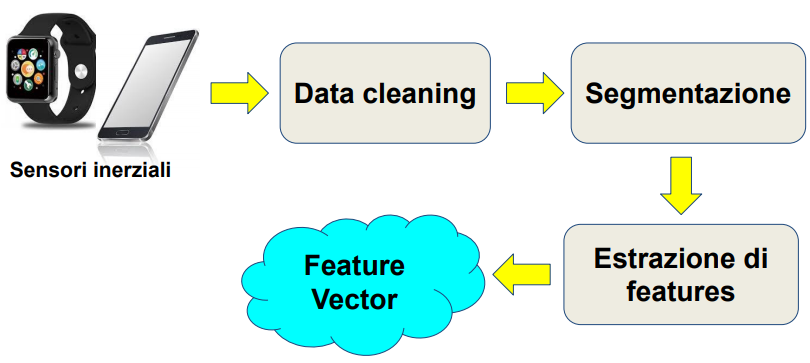
\includegraphics[width=.6\textwidth]{images/MobiDEV/6. activity recognition/pre-processing pipeline.PNG}
    \caption{Pipeline pre-processing}
    \label{fig:pipeline}
\end{figure}

\begin{itemize}
    \item data cleaning: i dati dei sensori sono affetti da rumore e per poter rimuoverlo si utilizzano i filtri, come il filtro mediano:
    \begin{center}
        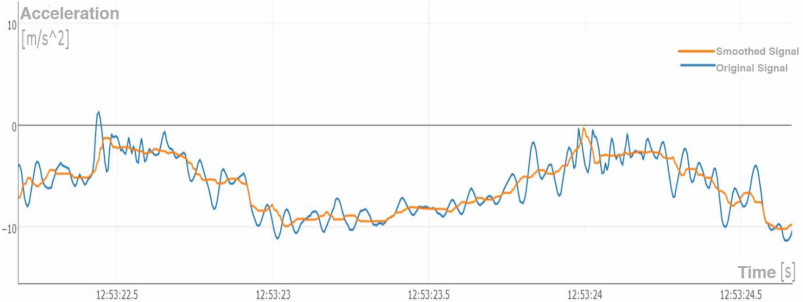
\includegraphics[width=\textwidth]{images/MobiDEV/6. activity recognition/data cleaning.PNG}
    \end{center}
    La linea arancione rappresenta il valore del filtro, quella blu rappresenta i dati grezzi. Ogni valore del segnale viene sostituito con la mediana considerando i valori nell'intorno
    \item segmentazione: il segnale viene diviso in segmenti temporali dove ogni segmento contiene i dati di tutti i sensori presi nello spazio temporale $t_1 t_2$. La tecnica più nota è lo sliding window. Abbiamo un insieme di finestre, dove una finestra può partire a metà della finestra precedente facendo un overlap (la seconda finestra può partire a metà della prima). 
    \begin{center}
        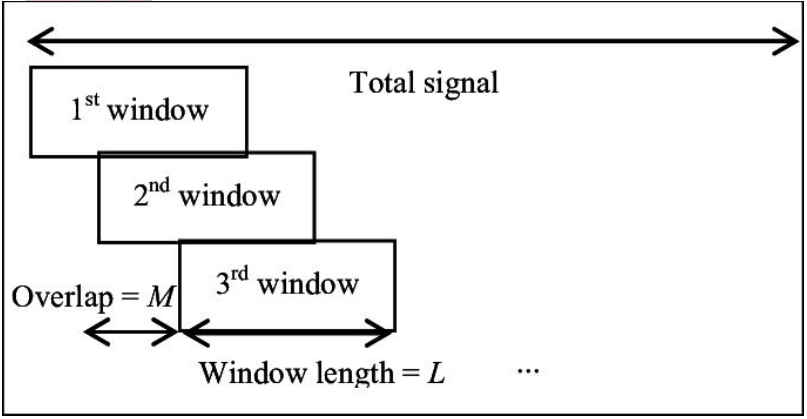
\includegraphics[width=.75\textwidth]{images/MobiDEV/6. activity recognition/segmentazione.PNG}    
    \end{center}
    Questo avviene perché andremo a classificare ognuna di queste finestre. Se le finestre sono affiancate senza overlap rischiamo che ci sia un'azione caratteristica che finisca a cavallo tra due e non riusciamo a riconoscerla. 
    \\ Se consideriamo attività semplici (camminare, stare seduti), di solito la finestra è di 3 o 4 secondi con un overlap del 50\%. Attività più complesse come lavare i piatti, richiedono una finestra più lunga. La dimensione della finestra può essere scelta anche in base a quanto "real-time" vuole essere il sistema 
    \item feature extraction: dai segmenti estraiamo informazioni per creare i vettori, i \textbf{feature vector}.
    
\end{itemize}

\subsection{Features}
Ci sono due tipi di feature, basate:
\begin{itemize}
    \item sul tempo: caratteristiche del segnale che riflettono il suo andamento nel tempo (es: media, varianza, ecc.)
    \item sulla frequenza: caratteristiche del segnale che riflettono la sua periodicità
\end{itemize}

\subsubsection{Generazione del feature vector}
Per ogni dispositivo mobile dell'utente si calcolano le features per ogni sensore inerziale al suo interno. Le features vengono concatenate per generare un vettore n-dimensionale, dove n è il numero di features calcolate. Le features sono solitamente grandi un centinaio. I range di valori delle diverse features possono variare significativamente.

\subsubsection{Feature scaling}
Per costruire un modello di riconoscimento robusto, abbiamo due tecniche:
\begin{itemize}
    \item normalizzazione: vengono normalizzati i range delle features e i valori sono scalati nel range [0,1]. È utile per rappresentare i dati usando una scala comune
    \item standardizzazione: cerca di riportare feature con range diversi, su una distribuzione simile. I valori sono centrati in 0. È particolarmente adatta se i dati hanno una distribuzione gaussiana 
\end{itemize}

Nell'ambito dell'activity recognition, non sempre normalizzare le features migliora il riconoscimento. Va valutato empiricamente se normalizzare e come. 

\section{Riconoscimento di attività: classificazione}
Abbiamo ottenuto i dati dei sensori divisi in segmenti e la notazione delle attività (etichette). La lunghezza dei segmenti dei dati non combacia con la lunghezza dei segmenti delle attività svolte. 
Serve un modo per associare un'etichetta ad ogni segmento. 
\begin{center}
    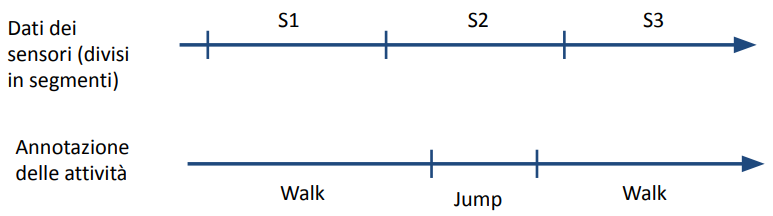
\includegraphics[width=.7\textwidth]{images/MobiDEV/6. activity recognition/labeling dei segmenti.PNG}
\end{center}

La soluzione più comune è associare l'attività prevalente del segmento. Ad esempio in S2, l'attività prevalente è Jump. In alcune situazioni, questa tecnica non funziona.

\subsection{Algoritmi di machine learning "noti" in AR}
Una volta etichettati i segmenti possiamo addestrare il classificatore. 
Tra gli algoritmi di classificazione, i più usati sono:
\begin{itemize}
    \item Support Vector Machine (SVM): supponiamo di avere 2 attività. Pallini neri attività 2, pallini bianchi attività 1. Lo scopo è di trovare un iperpiano che cerca di dividere al meglio gli esempi dell'attività 1 da quelli dell'attività 2.
    Bisogna quindi trovare la retta che distingue meglio le attività
    \begin{center}
        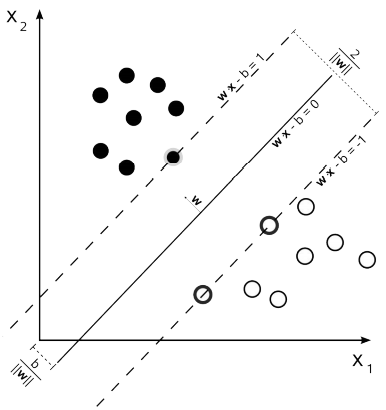
\includegraphics[width=.4\textwidth]{images/MobiDEV/6. activity recognition/svm.PNG}
    \end{center}
    \item Random Forest (basati su Decision Tree): il decision tree è un albero costruito in fase di training. Ogni nodo di questo albero è una condizione su una specifica feature (ad esempio valore dell'accelerometro $<$ 34). 
    Sono condizioni calcolate automaticamente in base ai dati di training. Le foglie di questo albero sono le attività. Si parte dalla radice e si passa attraverso l'albero in base alle condizioni che si trovano in ogni nodo.
    \begin{center}
        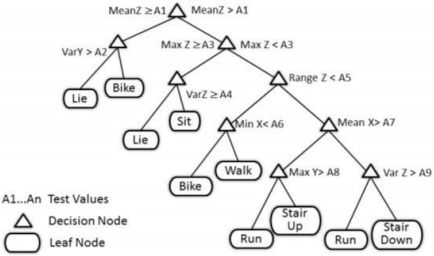
\includegraphics[width=.7\textwidth]{images/MobiDEV/6. activity recognition/decision tree.PNG}
    \end{center}
    Il random forest è una foresta di alberi di decisione. Il feature vector attraversa tutti i decision tree. Ogni albero di decisione è formato in modo randomico ed ognuno arriva alla propria predizione di attività. Attraverso un majority-voting viene presa l'attività prevalente tra tutti i decision tree. 
    \begin{center}
        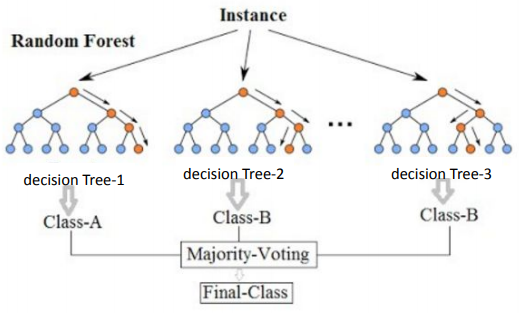
\includegraphics[width=.7\textwidth]{images/MobiDEV/6. activity recognition/random forest.PNG}
    \end{center}
    \item Reti neurali: ci sono tecniche di deep learning che permettono di calcolare le feature in modo indipendente. 
    Per estrarre le feature in modo affidabile, sono necessari molti dati
     \begin{center}
        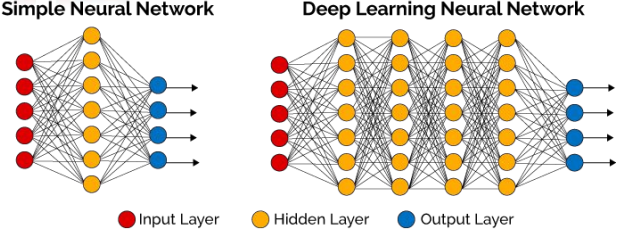
\includegraphics[width=.7\textwidth]{images/MobiDEV/6. activity recognition/reti neurali.PNG}
    \end{center}
\end{itemize} 

\subsection{Modello di riconoscimento}
Il modello di riconoscimento può essere:
\begin{itemize}
    \item personalizzato: allenato solo con dati dell'utente che utilizza il sistema. È molto accurato, ma non è realizzabile
    \item generalizzato: allenato usando dati di utenti diversi da colui che usa il sistema. Il training viene fatto una volta sola, ma il riconoscimento spesso è meno accurato. 
    Le API di Google e Apple adottano questo modello
\end{itemize}

L'ideale sarebbe avere un modello che combini i vantaggi dei due modelli: il training set viene creato inizialmente con un set di utenti diversi da colui che utilizza il sistema e poi viene chiesto all'utente di annotare una piccola porzione di dati per personalizzare il riconoscimento.

Dobbiamo capire se fare il riconoscimento:
\begin{itemize}
    \item offline: raccoglie i dati per un certo periodo e successivamente fa il riconoscimento
    \item online: processa i dati per riconoscere le attività in real-time. Lato online abbiamo pro e contro:
    
    \begin{table}[!ht]
        \centering
        \begin{tabular}{|p{.4\textwidth}|p{.4\textwidth}|}
            \hline
            \multicolumn{2}{|c|}{\textbf{Lato server}} \\
            \hline
            \textbf{pro} & \textbf{contro}\\
            \hline
            capacità computazionali elevate & grosso overhead in termini di comunicazione di rete \\
            \hline
        \end{tabular}
    \end{table}
    \begin{table}[!ht]
        \centering
        \begin{tabular}{|p{.4\textwidth}|p{.4\textwidth}|}
            \hline
            \multicolumn{2}{|c|}{\textbf{Lato mobile}} \\
            \hline
            \textbf{pro} & \textbf{contro}\\
            \hline
            miglior supporto al riconoscimento real-time & bisogna creare modelli di riconoscimento che possano girare efficientemente su dispositivi mobili \\
            \hline
        \end{tabular}
    \end{table}
\end{itemize}

Nei dispositivi mobili, il modello deve essere creato offline usando un training set (esistono svariati tool di machine learning che permettono di farlo) e ci sono apposite librerie che caricano il modello e lo usano per riconoscere in tempo reale le attività. 
Per poter creare e deployare il modello è necessario usare la stessa SDK. 
\\ Le SDK più famose sono:
\begin{itemize}
    \item Weka per Android
    \item CoreML per iOS: si può processare un modello offline ad esempio con librerie di Python, viene validato e una volta soddisfatti lo si può convertire in un formato apposito per CoreML e poi può essere deployato sull'applicazione ed utilizzato per il riconoscimento
    \item TensorFlow Lite per deep learning che può essere integrato sia in Android che in iOS
\end{itemize}

Un tool di Apple che fa parte di XCode e che permette di addestrare un classificatore senza dover scrivere codice è CreateML.

\subsection{Uso del modello}
Una volta che il modello è stato addestrato viene usato nel seguente modo:
\begin{itemize}
    \item il dispositivo acquisisce lo stream di dati dai sensori
    \item segmenta lo stream
    \item per ogni segmento estrae il feature vector
    \item il feature vector viene dato al classificatore che restituisce l'etichetta
\end{itemize}

\subsection{Il risultato del classificatore}
Il classificatore non restituisce solo l'attività ma una distribuzione di attività. 
Ad esempio abbiamo due distribuzioni di probabilità:
\begin{itemize}
    \item Caso 1: $<A, 0.5> <B, 0.4> <C, 0.1>$ 
    \item Caso 2: $<A, 0.5> <B, 0.25> <C, 0.25>$
\end{itemize}
In entrambi i casi l'etichetta più probabile è A, anche se nel primo caso il classificatore è più incerto (A con confidenza 0.5 e B di 0.4). \\
In base alla situazione si può decidere cosa fare del risultato: 
\begin{itemize}
    \item usare sempre l'etichetta con confidenza più alta
    \item definire qualche metrica per decidere quando prendere per buono il risultato del classificatore
\end{itemize}
\rhead{Lezione 10 - 15 aprile}
\begin{comment}
Chicco

\section{Cos'è il contesto?}
Le applicazioni tradizionali non sono in grado di capire il contesto di una richiesta. \\
Le richieste ai sistemi tradizionali devono essere fatte esplicitando tutti i parametri del contesto. \\
In un ambito context aware posso eliminare la richiesta dei parametri a percepirli da altre informazioni (Se voglio andare da X a Y, X potrebbe essere il punto dove mi trovo e Y potrebbe essere un luogo dove ho un meeting, se ho condiviso calendar ecc ecc)\\
La comunicazione con il computer è difficile:
\begin{itemize}
    \item ci sono interfacce limitate, specialmente da mobile
    \item abbiamo bisogno di un meccanismo automatico per acquisire e trasmettere il contesto della nostra richiesta
\end{itemize}
Ci sono molte definizioni di contesto e anche molte interpretazioni in ambito psicologico, filosofico o informatico.\\
Dal vocabolario il contesto è:
\begin{quote}
    un insieme di circostanze o fatti che circondano un particolare evento o situazione (nel nostro caso una mobile service request)
\end{quote}
In informatica sono state proposte diverse definizioni:
\begin{itemize}
    \item luogo, tempo, persone circostanti, stagioni, temperatura...
    \item luogo, ambiente, identità e tempo
    \item stato d'animo, livello di attenzione, luogo, tempo, oggetti e persone circostanti
\end{itemize}
Una definizione comune è:
\begin{quote}
Context is any information that can be used to characterize the situation of
an entity. An entity is a person, place, or object that is considered relevant to
the interaction between a user and an application, including the user and
applications themselves.
\end{quote}
Semplificando:
\begin{quote}
    Tutti i dati utili ad adattare il servizio (nel momento in cui si usufruisce di questo servizio)
\end{quote}

\section{Classificazione del contesto}
TABELLA

\section{Contesto temporale}
Si considera non solo l'ora, il giorno, il mese la stagione.. ma soprattutto la storia del contesto gioca un ruolo importante. Ossia possiamo fare molto di più tenendo traccia del contesto (storia del contesto): possiamo derivare un nuovo contesto o predire il contesto

\section{Adattività}
La proprietà di un sistema di adattarsi a un dato contesto per fornire un servizio/esperienza migliore.\\
Un sistema context-aware acquisice i dati per adattare automaticamente il suo comportamento.\\
Molto importante in ambito mobile per:
\begin{itemize}
    \item cambiamenti nella connessione
    \item cambiamenti nella batteria
    \item cambiamenti della situazione dell'utente
    \item cambiamenti nell'ambiente
\end{itemize}
\subsection{Tipi di adattività}
\begin{itemize}
    \item adattare le funzionalità: mostrare o nascondere funzionalità, cambiare il data flow, aumentare la cache, spostare più computazione server side ecc ecc
    \item adattare i dati: il sistema potrebbe fornire dati più o meno precisi, qualità maggiore o inferiore
\end{itemize}

\section{Ottenere il contesto dai dati}
\begin{itemize}
    \item Basso livello: 
    \begin{itemize}
        \item Dati acquisiti dai sensori o altri sensori: dati raw dai sensori, informazioni explicite dal profilo utente, capacità del dispositivo mobile
        \item Ottenuti da una elaborazione semplice e/o dalla funzione di dati raw: stima della banda di rete facendo la media su valori campione in uno slot di tempo
    \end{itemize}
    \item Alto livello:
    \begin{itemize}
        \item Derivati applicando inferenze sui dati di basso livello: il mood delle persone posso ricavarlo dalle attività delle persone, dal GSR rilevato al polso ecc ecc
        \item possiamo ottenere info di alto livello riutilizzando info di alto livello
    \end{itemize}
\end{itemize}

\subsection{Metodi di inferenza}
Due categorie di approcci: statistici e simbolici.
I simbolici sono basati sulla logica (horn, logica descrittiva, ecc), mentre gli statistici sono quelli dati dal machine learning (classificazione e clustering)

\subsection{Riconoscimento delle attività}
....

\section{Rappresentare il contesto}
È importante per diverse ragioni: 

________________________________________
Fabbio

\textbf{Unserstandig context}
Le applicazioni tradizionali non sono i ngrado di capire il contesto. Ad esempio un servizio nell'ambito del pervasive. Nei sistemi tradizionali se faccio una richiesta devo specificare troppe cose. 
In un ambito context aware il sistema, in base a diversi parametri sia di preferenza personale sia di dati presi dall'ambiente riesce a fornirmi un'esperienza adeguata a quella che cerco senza che io gli specifichi le cose.
Nei sistemi pervasivi si vuole chiedere il meno possibile al sistema ma far si che sia il sistema ad anticipare quello che vogliamo

\textbf{Defining context}
In generale si vorrebbe poter dire con la voce

\textbf{Early defintions}
In alcuni casi si elenca cosa significa "contesto".
(slide)
(F1,f2,f3 erano puntatori ad articoli)

\textbf{A common definition}
(Definizione sulla slide) TUtta l'informazione che riguarda una persona, posto, oggetto ma non in generale...

\textbf{Classification of context}
(slide)
via celoria 18

\textbf{Temporal context}
Il tempo svolge un ruolo fondamentale. La storia del contesto svolge un ruolo fondamentale. Può essere utile per capire le abitudini.

\textbf{Adaptiveness}
L'obiettivo dell'acquisizione del contesto è l'adattività del sistema al contesto. 
Vogliamo un sistema che cambia nel tempo (Si adatta).
Dunque acquisisce dati da vari fattori e cambia il suo comportamento di conseguenza. 

\textbf{Adaptive video streaming}
Progetto del prof per ottimizzare la fruizione del video adattandolo al contesto.  Idea che dati di contesto arrivano da più fonti.

\textbf{Types of adaptiveness}
\begin{itemize}
    \item Adapting functonality: A seconda del contesto il sistema ti mostra solo alcune funzionalità del servizio.
    \item adapting data: Il sistema non agisce sulle funzionalità ma sui dati trattati. 
\end{itemize}

\textbf{Obtaining context data}

\textbf{inferring context data}
High-level context: 

\textbf{Inference methods}
Due categorie principali
statistici: Machine learning. DUe task più noti classificazione e clustering
simbolici: Basati sulla logica

\textbf{Activity recognition}
Fase di preprocessing: in cui si prendono i dati grezzi e si cerca di ridurre il rumore
suddivisione in finestre temporale
aggregazione dei segnali

\textbf{Hybrid reasoning}

\textbf{Context representation}
Perchè dovremmo rappresentarlo? I dati innanzitutto sono ottenuti da sorgenti etereogenee. E' possibile che queste sorgenti utilizzino diverse semantiche. Non c'è uno standard per i dati di contesto quindi c'è una mancanza di semantica condivisa...

\textbf{Requirements}
________________________________

омар 

Le applicazioni tradizionali non sono in grado di capire il contesto. Se faccio una richiesta ad un sistema tradizionale devo specificare un sacco di cose sul contesto, in contrasto con un sistema context-aware che può intuire molte di queste.
Dunque, in generale, è possibile rendere più smart i servizi utilizzando il contesto.
Quando ci si trova ad utilizzare un sistema mobile o pervasivo si vuole interagire il meno possibile con il sistema, per questo motivo questi servizi sono importanti.
Per contesto si intende: location, time, surrounding people, ecc...
Ciascun articolo utilizza una definizione diversa.

Una tra le varie definizioni che spesso si cita è quella di Anind Dey: è tutta l'informazione che riguarda una persona, un posto o un oggetto, ma non in generale. Stiamo sviluppando sistemi per offrire servizi anticipando i bisogni. Nella situazione in cui un'entità vuole usufruire di un servizio, tutto ciò che caratterizza quella situazione può essere utile per adattare il servizio e lo chiamiamo contesto.

Qualcuno ha cercato di farne una tassonomia, visto che le componenti del contesto sono molte, ma questo ovviamente non è scolpito nella pietra. Sono dinamici ed in divenire, poiché si possono sviluppare nuovi metodi per capire una certa dimensione.

Il contesto temporale svolge un ruolo fondamentale nell'adattamento. Non soltanto il mese, la stagione, ecc..., ma soprattutto la storia del contesto nel tempo, avendo l'autorizzazione di conservarlo. Se riesco a correlare la storia del contesto posso capire le sue abitudini rispetto a cosa fa quel giorno, in quell'ora, ecc... Utile quindi tenere traccia del contesto per dedurre nuovo contesto e predire contesto. L'idea è quindi che il sistema proponga qualcosa senza effettuare alcuna richiesta.

L'obiettivo dell'acquisizione dei dati del contesto è l'adattività del sistema pervasivo. Vogliamo un sistema che cambia nel tempo. Vogliamo che il sistema cambi il comportamento ed impari a cambiarlo meglio, in alcuni casi. Acquisisce i dati e modifica il comportamento per ottimizzare il servizio. Questo è importante anche in ambito mobile per capire i cambi nella rete, nella fruizione dell'energia, l'interfaccia che si sta usando al momento, la situazione in cui ci si trova e cambiamenti dell'ambiente. Tutte queste sono adattamento e si può fare a diversi livelli. 

Due modi per adattare i servizi:
- adattare la funzionalità offerta, a seconda di quel che sistema capisce fa vedere solo determinate funzionalità, aumentare cache, muovere computazioni server side, ecc.
- adattare i dati, usando dati più o meno preicisi

Quando si parla di ottenere dati di contesto:
- dati di baso livello: acquisiti direttamente dai sensori o altre sorgenti. Vado semplicemente a leggerli. Consideriamo anche di basso livello i dati ottenuti attraverso un semplice processing o una fusione (ad esempio la media).
- dati di alto livello: contesto ottenuto nell'applicare metodi di inferenza sul contesto di basso livello, che possono anche essere piuttosto complicati. Posso utilizzare contesto di alto livello per derivare altro contesto di altro livello.

Quello di basso livello si acquisisce con un accesso diretto attraverso l'architettura. Alto livello ha bisogno di applicazione di metodi di inferenza sul basso livello. Questi modi di inferenza possibili sono:
- approcci statistici, machine learning. I due task più noti sono quelli della classificazione (dato un insieme di dati e cateogrie, capire a quali categorie questi dati fanno riferimento) e clustering (cerca di mettere insieme insieme di dati, per esempio per scoprire nuove attività che non fanno parte delle categorie e creare una nuova categoria).
- approcci simbolici, basati sulla logica.

Se riesco a capire che attività una persona sta facendo, riesco ad adattare meglio il servizio che devo fornire. Questo è ad alto livello. C'è una fase di preprocessing, qindi prendiamo i dati grezzi dai sensori e cerchiamo di ridurre il rumore, rendendo più evidenti i fenomeni che devono caratterizzare. Si suddividono i fenomeni in finestre temporali e si aggregano i segnali, calcolando le caratteristiche dei segnali in quei segmenti. Dopodiché si cerca di allenare un certo modello.
Facciamo fare attività a degli utenti, annotiamo le ground truths, quindi associamo delle misure che abbiamo acquisito con una verità, quindi alla cetegoria che sappiamo qual è. ALleniamo il modello con i dati e con la categoria osservata, finché non sarà pronto. A questo punto, lo posso utilizzare ed il sistema, guardando i dati fa una predizione senza che nessuno osservi la categoria, tipicamente associando una probabilità/confidenza a questa predizione.
Ci sono metodi completamente basati su approcci simbolici anche per il riconoscimento di attività.
I metodi più efficaci per questo tipo di inferenze si sono rilevati quelli statistici, con la difficoltà che i metodi logici hanno di rappresentare l'incertezza.
Ci sono anche molti modi di combinare i due metodi di inferenza. Esistono diversi modi epr farlo, uno dei quali è metterli in sequenza: usiamo lo statistico, facciamo una predizione e poi confrontimao la predizione fornita (le due o tre su cui è incerto il modello statistico) e proviamo a vedere le regole simboliche, utilizzando il contesto.
Dai dati del sensore possiamo andare a fare ragionamenti di common sense reasoning, ad esempio dove si svolge tipicamente l'attività. Questi ragionamenti possono aiutare. Quello che facciamo con questi ragionamenti è astrarre, cosa che le macchine fanno ancora fatica a fare. L'uso di questo aiuta a raffinare le predizioni.

I dati sono ottenuti da sorgenti eterogenee. È anche psosibile che utilizzino diversi linguaggi per fornire questi dati. Non c'è una semantica condivisa di solito (standard per tutti i tipi dati di contesto). Serve un common representation language e se voglio automaticamente rielaborarlo ho bisogno di una rappresentazione formale in qualche linguaggio. 

I requisiti di un modello di rappresentazione dei dati sono:
- eterogeneità dei dati
- ci piacerebbe riuscire a collegarli, poiché ci sono correlazioni nei dati (catturare relazioni)
- voglio rappresentare la storia
- voglio rappresentare il livello di incertezza
- voglio riuscire a fare ragionamento
- vorrei che fosse facilmente utilizzabile ed efficiente

Per singole applicazioni molto semplici che non devono condividere dati con altri si può usare un sistema molto semplice: modello Flat. Utilizzo una chiave e un valore. Nessuna struttura. Utilizzato da molti application server commerciali. Qualcuno ha cercato di arricchirli un po' con delle gerarchie di attributi usando strutture con XML con un opportuno schema. Il modello flat dà usability, efficiency (poiché reperire questi dati è immediato) e più o meno anche eterogeneità ed estensibilità.

Proposta intermedia: se vogliamo catturare relazioni tra i dati di contesto possiamo usare CML (non più utilizzato), che è una variante dell'E/R in cui sono stati introdotti dei simboli particolare tipici della rapprestanzione delle informazioni di contesto derivanti anche dai sensori. Questo va a migliorare, rispetto al flat, la capacità di rappresentazione delle relazioni e delle dipendente del contesto. Seppur in forma limitata consente anche di rappresentare l'incertezza, tuttavia non ha un sistema di ragionamento automatico. Cattura qualche aspetto temporale, ma in modo limitato. Al massimo c'è una memorizzazione del tempo, non c'è un ragionamento, fino a SQL 2011 (?).

Ontologie: strettamente legato alla rappresentazione simbolica. Per ontologia si intende una specifica formale di uan concettualizzazione (come E/R) condivisa. Cerchiamo di dare una specifica formale ai dati del contesto e alla conoscenza comune in modo condiviso. Una votla d'accordo, tutte le applicazioni possono usarla e se riusciamo a mettere nel midleware qualcosa che fa ragionamento su queste cose, possiamo arrivare a realizzare sistemi intelligenti. Il linguaggio che si usa è una famiglia di linguaggi che si chiama logiche descrittive, che è un sottoinsieme della logica del primo ordine e permette di modellare domini complessi. Ha semantica formale e fa ragionamento automatico e capire se per esempio è stata fatta una descrizione incosistente. Il lignuaggio è OWL per definire ontologie, proposto da w3c (specifica logica descrittiva in cui sono stati selezionati degli operatori). UN modello di questo genere supporta:
- consistenza
- relaization, ho insieme di osservazioni che non sono concetti. Sono contesto di basso livello. Dato un insieme di osservaizoni va a vedere qual è la categoria che cattura queste osservazioni. attività di inferenza basata su regole logiche del contesto
- ???
Ci sono strumenti per fare questo.

Le architetture possono anche essere miste. possiamo fare una prima derivazione di contesto di alto livello con machine learning, capiamo l'azione base che sta facendo, la mettiamo insieme ad altri dati che ci arrivano da altre sorgenti, le metto insieme facendo una forma di aggregazione e poi la passo ad ontologia che mi dice a quale attività corrisponde.

Non è la soluzione definitva. Non sono nate per supportare incertezza, ci sono tentativi. L'incertezza nella rapprestentzaione dei dati di contesto è da investicare, così come i dati storici. Se ontologia complessa non può essere fatta su dispoitivi, ma dev'essere fatta cloud just in time.

in questo momento non esiste un vero ep orpio supporto middleware che includa tutto questo, tranne proposte in ambito di ricerca. I metodi di inferenza si stanno ancora raffinando, anche se la più efficiente è machine learning con correzioni del simbolico. Supporto middleware dovrebbe integrare:
-
-
-
-
-





\end{comment}
\rhead{Lezione 11 - 19 aprile}
\begin{comment}
    
    Omar
    Data privacy
    Importante nell'ambito dei sdp perché trattano dati che potrebbero essere sensibili.
    Cos'è la privacy? Il diritto di essere lasciato in pace, in sintesi.
    Per passare da questo alla data privacy, occorre capire cosa sono i dati personali.
    GDPR dal 2018, nell'articolo 4 si definisce dati personali come: dati/informazioni che riguardano un individuo identificato o identificabile (più debole). La capacitià di un individuo di controllare il rilascio e la distribuzione dei propri dati.
    Quasi-identifier: informazione che combinata con altra informazione può restringere i candidati ai quali i dati corrispondono.

    Servizi online: gruppo di utenti che mandano richieste. L'avversario (potrebbe essere il fornitore del servizio) guarda i dati nelle richieste (magari anche anonime, con username) e, avendo accesso all'external knowledge, si ha violazione di privacy quando da una parte si hanno i dati personali e dall'altra i dati dell'utente, associandoli.
    
    Geo-sn
    Utente, anche non essendo taggato diretatmente ad una risorsa, può essere associato attraverso la location.
    SLIDE
    
    Nei pervasivi:
    Più dati, più esposizione.
    Nuovi tipi di dati, quindi nuovi modi per re-identificare le persone e derivare dati sensibili
    Rispetto ai dati tabellari, abbiamo stream continui di dati e le sequenze possono essere correlate
    Meno consapevolezza delle persone, più difficile esprimere consenso e monitorare
    Mancanza di interfacce per controllare le preferenze
    
    Come possiamo proteggerci:
    GDPR:
    - garantire security
    - privacy by design: non progettare prima e poi pensare alla privacy, pensare alla privacy mentre si progetta
    - pseudonimitazion
    - data minimization
    
    Transaprency: non nascondere all'utente come vengono trattati i loro dati. Avere log dettagliati, blockchain è un modo
    Unlinkability: separare informazioni e non renderle riassociabili, tecniche su slide.
    Intervenability: dev'esserci un modo di intervenire nel processo. Break Glass procedures, data rectification, right to be forgotten, manual override
        
    GDPR non si applica su informazioni anonime
    
    Questi 3 sono importanti oltre a sicurezza e altri 2
    
    Data minimization: raccogliere dati alla precisione che serve per il servizio che si fornisce e non si tengono per sempre, per quello che serve e usarli per lo scopo dichiarato.
    pseudonimitazion: modo di fare unlinking, salvando un id e avendo da qualche parte il mapping. Non è anonimizzazione.
    
    Location k-anonimity: allargo la regione da avere k - 1 utenti in più e anziché mandare la posizione esatta mando l'area
    Un server fidato sa dov'è l'utente e può filtrare la risposta per dare quella più appropriata all'utente, visto che l'area è più imprecisa
    

    
    
    
    -----------------
    Cos'è la privacy?
    Il diritto di essere lasciato in pace.
    Cos'è la data privacy? 
    Abilità di controllare il rilascio, l'uso e la distribuzione di personal data (qualsiasi informazione a cui sono associate un individuo identificato o identificabile)
    
    
    
    
    
    
\end{comment}

\chapter{Introduzione a Swift}
\lhead{Introduzione a Swift}
\rhead{Lezione 12 - 22 aprile}
\begin{center}
    \textbf{--------- Lezione 12 - 22 aprile 2021 ---------}
\end{center}

\section{Swift}
Swift è un linguaggio di programmazione realizzato da Apple.
È un linguaggio moderno, recente anche rispetto ad linguaggi di programmazione come C, Java C\#, Dart.

Gli obiettivi di chi crea un nuovo linguaggio di programmazione sono:
\begin{itemize}
    \item evitare/ridurre gli errori più comuni del programmatore
    \item aumentare la compattezza del codice
    \item migliorare la leggibilità del codice
    \item migliorare le prestazioni
\end{itemize}

Le caratteristiche principali di Swift sono:
\begin{itemize}
    \item multi piattaforma (iOS, watchOS, macOS, tvOS, ecc.)
    \item compilato
    \item supporta due paradigmi di programmazione: 
    \begin{itemize}
        \item Object Oriented
        \item Funzionale
    \end{itemize}
    \item si possono creare applicazioni utilizzando combinazioni di Swift, Objective-C, C e C++
\end{itemize}

\section{Programmazione procedurale in Swift}
Parole riservate:
\begin{itemize}
    \item \textbf{var} definisce una variabile
    \item \textbf{let} definisce una costante
\end{itemize}
L'assegnamento viene fatto con "=", mentre il punto e virgola al termine di ogni istruzione è opzionale ed è preferibile ometterlo, per questioni di stile.

Swift è un linguaggio di programmazione fortemente tipizzato. 
Si può evitare di specificare il tipo di una variabile nel momento in cui essa viene specificata ed il tipo viene inferito in automatico, ma non può essere cambiato a runtime (come invece succede in JavaScript).
\begin{Swift}
    var a = 5 //this is Int
    var b:Int = 3 //this is explicitly an Int
    var c = a+b //this is Int
    var d = "hello!" //this is a String
    c = d; //this gives a compile-time error
\end{Swift}

Come avviene in altri linguaggi si può effettuare la conversione di tipi attraverso determinate funzioni.
Ad esempio per convertire un intero in stringa ci sono due modi:
\begin{Swift}
    var studentNumber = 50
    let label = "Ci sono " + String(studentNumber) + " studenti"
    //prima conversione
    let label2 = "Ci sono \(studentNumber) studenti"
    //seconda conversione
\end{Swift}

\subsection{Tuple}
Una variabile può essere associata ad una tupla di valori, es:
\begin{Swift}
    let httpError = (404, "Not Found") //tupla di valori
    //in questo caso error e' di tipo (Int, String)
\end{Swift}
Per poter leggere i valori di una tupla si può operare nel seguente modo:
\begin{Swift}
    print(httpError) //prints "(404, "Not Found")"
    //modo 1.
    let (statusCode, statusMessage) = httpError
    print(statusCode) //prints 404
    print(statusMessage) //prints "Not Found"
    //modo 2.
    let (statusCodeAgain,_) = httpError; /*just read the 
    error number, not the type
    note: in the line above I have used the "_" symbol 
    meaning "I don't care about the second value"*/
    print(statusCodeAgain) //prints 404
    //modo 3.
    let statusCodeAgainAgain = httpError.0
    print(statusCodeAgainAgain) //prints 404
    let statusMessageAgain = httpError.1
    print(statusMessageAgain) //prints "Not Found"
\end{Swift} 

La differenza tra tupla e classe è il fatto che una tupla ha solo lo stato, mentre una classe ha sia lo stato che il comportamento. 
Le tuple si usano per insieme di dati da usare localmente nel codice, ad esempio valori di ritorno delle funzioni. In altri casi si usano le classi o le strutture.

\subsection{Valori opzionali}
Di default una variabile non può assumere un valore nullo.
Possiamo specificare una variabile come \textbf{optional} per indicare che può assumere il valore nullo:
\begin{Swift}
    var i:Int? = nil 
\end{Swift}
Le variabili opzionali sono di un tipo diverso rispetto alle controparti non-opzionali, ad esempio Int? è diverso da Int. 
Se una funzione prende in input Int, non posso passarle Int?, però vale il contrario. 

Ho una serie di restrizioni quando ho una variabile opzionale:
\begin{itemize}
    \item non posso usarla nelle espressioni (non posso fare a+b se una delle due variabili è opzionale)
    \item non posso accedere ai metodi o accedere alle proprietà
\end{itemize}
Esistono vari metodi per estrarre ("unwrap") il valore non-opzionale da una variabile opzionale o comunque per gestire i tipi opzionali. 
In Java se abbiamo un attributo a di una classe che è null e proviamo a leggerlo, viene dato un NullPointerException.

Ci sono diversi metodi per fare unwrapping:
\begin{itemize}
    \item forced unwrapping: mettendo un ! dopo una tipo opzionale, si va a leggere quel tipo come se non fosse opzionale. Se si usa questa sintassi su una variabile che è nil, viene generata un'eccezione a runtime, quindi bisogna sempre controllare prima che non sia nil.
    \begin{Swift}
        var a = 1 //non-optional
        var b = Int("123") //optional
        var c:Int 
        c = a+b /*this is a is a compile-time error b cannot 
        be used in an expression because it could be nil*/
        //solution:
        if b != nil {
         //we use "!" to unwrap the value
         c = a+b!
        }
        /*force unwrapping of a nil variable generates 
        a runtime exception*/
    \end{Swift}
    \item optional binding: si usa un costrutto sintattico comunemente detto "if let". 
    \begin{Swift}
        var possibleNumber = "123"
        var numberOptional = Int(possibleNumber)
        /*next line: check if numberOptional is nil, 
        if not, assign it to numberNonOptional and run 
        the if condition. Otherwise run the else 
        condition.*/
        if let numberNonOptional = numberOptional {
         print(numberNonOptional) //prints 123
        } else {
         print("cannot convert")
        } 
    \end{Swift}
    La condizione dell'if è verificata se la variabile che vogliamo controllare non è nil ed in quel caso all'interno del costrutto if abbiamo un riferimento ad un'altra variabile, dello stesso tipo ma non opzionale
    \item implicitly unwrapped optionals:
    \begin{Swift}
        var a: String!
        var b: String = ""
        b = a /*generates a runtime error: I am assigning a 
        nil value to a non-optional variable*/
        a = "ciao"
        /*next line: I can use b as if it is not 
        optional (note, I am not using the !)*/
        b=a;
    \end{Swift}
    A volte è possibile avere una variabile optional che ha sempre un valore. Se definisco una variabile con "!" questa è optional, ma la posso usare come se non lo fosse
    \item optional chaining: con una variabile opzionale non è possibile accedere né alle proprietà né richiamare i metodi, ma è possibile richiamare metodi e proprietà con una sintassi particolare, attraverso ?, in modo tale che, se la variabile è nil, viene restituito nil, senza generare eccezioni. I valori ritornati sono sempre opzionali
    \begin{Swift}
        var user: Person?
        var n = "" //an empty non-optional string
        n=user.name /*compile time error: cannot use a 
        property for optional variable user*/
        n=user!.name //run-time exception if user is nil
        n=user?.name /*compile time error: name is a 
        non-optional property, but when used with 
        optional chaining can return nil, so it cannot 
        be assigned to non-optional variable n*/
        var m: String?
        m = user?.name
    \end{Swift}
    \item nil-coalescing operator: l'operatore ?? viene utilizzato per rendere più breve un'operazione comune: data una variabile opzionale a, restituire il valore di a se a non nil, altrimenti un valore b
    \begin{Swift}
        let defaultColorName = "red"
        var userDefinedColorName: String? // defaults to nil
        var colorNameToUse = userDefinedColorName ??
                             defaultColorName
        /*meaning: if userDefinedColorName is not nil (which 
        is not the case in this example), then colorNameToUse 
        is userDefinedColorName. Otherwise colorNameToUse is
        defaultColorName*/
    \end{Swift}
\end{itemize}

La gestione delle variabili opzionali comporta una sintassi più complicata e la necessità di passare da variabili opzionali a non opzionali.
\\ La sintassi, però, è utile per spostare un'eccezione, a livello di errore sintattico identificato, a tempo di compilazione, a differenza di Java che con un NullPointerException ci dà errore a run-time.

Alla fine il risultato è una riduzione degli errori di gestione delle variabili con valore nullo. 

\subsection{Operatori}
Sono molto simili agli operatori C:
\begin{itemize}
    \item unari (-a, !b)
    \item binari (a+b)
    \item ternari (a?b:c che significa "if a then b, else c")
\end{itemize}

In Swift il confronto tra due oggetti funziona con ==. L'operatore === confronta se due variabili puntano allo stesso indirizzo di memoria.
Non esistono gli operatori ++ e --.

\subsection{Gestione dell'overflow}
In Java l'overflow non causa l'eccezione ma un bug. 
\begin{Java}
    int a = Integer.MAX_VALUE - 1;
    int b = Integer.MAX_VALUE - 1;
    int c = a + b;
    System.out.println(c); //-4
\end{Java}
In Swift gli overflow generano un'eccezione a run-time. 
\begin{Swift}
    var a = Int.max
    var b = Int.max
    let c = a + b
    print(c) //error: Execution was interrupted
\end{Swift}

La gestione dell'overflow in Swift aiuta a risolvere il problema ed evita che l'errore si propaghi. Non previene un errore comune, ma ne limita gli effetti e lo rendo più semplice da risolvere. 

\subsection{Operatori di range}
Gli operatori permettono di creare rapidamente dei grupppi di interi o elementi contigui di un array.
\begin{Swift}
    for i in 1...5 {
        print(i)
    } //1, 2, 3, 4, 5
    for i in 1..<5 {
        print(i)
    } //1, 2, 3, 4
    let names = ["Anna", "Alex", "Brian", 
    "Jack"]
    for i in names[1...2] {print(i)} //Alex, Brian
    for i in names[...1] {print(i)} //Anna, Alex
    for i in names[2...] {print(i)} //Brian, Jack
\end{Swift}

\subsection{Collezioni}
Sono predefinite tre strutture dati principali:
\begin{itemize}
    \item array: possono essere definiti con $Array<Element>$ o $[Element]$
    \item set: sono definiti $Set<Element>$, non possono contenere duplicati. Abbiamo a disposizione gli operatori tipici insiemistici (unione, intersezione, ecc.)
    \item dictionary: sono analoghi alle mappe in Java, un insieme di coppie di elementi, in cui il tipo del primo e del secondo elemento sono definiti
\end{itemize}

\subsection{Selezione con costrutto guard}
Guida il programmatore a scrivere il codice in modo più leggibile. Il costrutto guard verifica che valga una determinata condizione ed esegue del codice nel caso in cui non sia valida.
Nel caso in cui non sia valida, si esce dalla funzione, si segnala un errore o si genera un'eccezione.
È un costrutto if in cui si considera solamente il caso in cui la condizione non sia verificata.
\begin{Swift}
    func divide(numerator: Int, denominator: Int) {
        guard denominator != 0 else {
            print("non si puo'")
            return
        }
        print(numerator/denominator)
    }
    
    divide(numerator:10, denominator: 2)
\end{Swift}


\rhead{Lezione 12 - 26 aprile}
\begin{center}
    \textbf{--------- Lezione 13 - 26 aprile 2021 ---------}
\end{center}

\section{Funzioni e closures}
Caratteristiche delle funzioni: 
\begin{itemize}
    \item possono avere più di un valore di ritorno (come le tuple)
    \item i parametri possono avere dei valori di default
    \item le funzioni sono un tipo di dato (un parametro di una funzione ad esempio può essere una funzione)

\end{itemize}
\begin{Swift}
    func greet(person:String) -> String{ //definizione 
        let greeting = "Hello, " + person + "!"
        return greeting
    }
    
    print(greet(person: "Sergio")) //richiamo la funzione
\end{Swift}

\subsection{I parametri}
In Java un parametro è caratterizzato dal nome e dal tipo.

In Swift, invece, ogni parametro ha 3 caratteristiche:
\begin{itemize}
    \item un argument label: specifica l'etichetta da usare quando si richiama la funzione
    \item il nome del parametro: nome della variabile da usare nell'implementazione della funzione
    \item il tipo del parametro
\end{itemize} 

Se non indichiamo la label abbiamo il nome della variabile (nella funzione) preceduto da "\_".

Le label hanno un valore sintattico: in Java non possiamo avere due funzioni che hanno la stessa signature (nome del metodo, l'elenco di tipi del metodo ed il valore di ritorno), in Swift invece la label fa parte della signature, quindi possiamo avere due metodi uguali con una label diversa.

I parametri possono avere un valore di default (opzionali) e per convenzione vengono messi dopo quelli necessari. 

Quando all'interno di una funzione voglio cambiare il valore di un parametro, devo andare a specificare la parola riservata \textbf{inout} e bisogna passare i parametri (quando si richiama la funzione) per riferimento. 

Le funzioni sono un tipo di dato, definito dal tipo dei parametri e del valore di ritorno. 
La funzione sum ad esempio associa un interno ad una coppia di interi. 
\begin{Swift}
    func sum(_ a: Int, _ b: Int) -> Int{
        return a + b;
    }
    
    func dif(_ a: Int, _ b: Int) -> Int {
        return a-b;
    }
    
    func f(theFunction: (Int, Int)->Int, _ a: 
    Int, _ b: Int) -> Int {
        return theFunction(a, b);
    }
    
    let a=5, b=3
    var operation = sum
    print(f(theFunction: operation, a, b)); //8
    operation = dif
    print(f(theFunction: operation, a, b)); //2
\end{Swift}

È possibile assegnare un nome nuovo ad un tipo come:
\begin{Swift}
    typealias Pippo = Int //posso usare Pippo al posto di Int
\end{Swift}
È molto utile quando si usano le funzioni come tipi.

\subsection{Ordinamento di un Array}
Per ordinare un Array, è necessario passare come parametro il criterio di ordinamento: 
\begin{Swift}
    func forward(first:String, second:String) -> Bool {
        return first<second
    }
    func backward(first:String, second:String) -> Bool {
        return first>second
    }
    
    let names = ["Carlo", "Daniele", "Ugo", "Bruno", "Sergio",
                "Mattia"]
    print(names.sorted(by: forward)) 
    //["Bruno", "Carlo", "Daniele", "Mattia", "Sergio", "Ugo"]
    print(names.sorted(by: backward))
    //["Ugo", "Sergio", "Mattia", "Daniele", "Carlo", "Bruno"]
\end{Swift}

È anche possibile definire una funzione dentro ad altre funzioni. La visibilità delle funzioni definite cambia, infatti non è possibile accedere ad una funzione definita all'interno di un'altra.


\subsection{Closures}
Sono simili ai blocchi in C e Objective-C e alle lamdba expression di Java. 
Servono per risolvere in modo più compatto alcuni problemi tipici di questi linguaggi come la gestione degli eventi.
Sono alla base della sintassi di SwiftUI.
Una closure concettualmente corrisponde a definire una funzione nel momento stesso in cui mi serve.

Indichiamo una closure tra parentesi graffe, indichiamo i parametri ed il valore di ritorno, poi usiamo la parola riservata \textbf{in} e indichiamo il procedimento
\begin{Swift}
    let names = ["Carlo", "Daniele", "Ugo", "Bruno", "Sergio",
    "Mattia"]
    print(names.sorted(by:{(first: String, second: String) -> 
                            Bool in
        return first<second}))
    //["Bruno", "Carlo", "Daniele", "Mattia", "Sergio", "Ugo"]
\end{Swift}

Ci sono diverse tecniche per ridurre il codice attraverso le closures:
\begin{itemize}
    \item type inference: quando definiamo una funzione da sola, dobbiamo definire tipi e parametri, se invece una closure è passata come argomento ad una funzione, il compilatore sa già quali tipi aspettarsi, dunque possiamo evitare di indicarli. 
    \begin{Swift}
    print(names.sorted(by:{first, second in
        return first<second
    }))
\end{Swift}
    \item implicit return: se una closure ha una sola istruzione, si può omettere il return
    \begin{Swift} 
        print(names.sorted(by:{first, second in 
                                first<second}))
    \end{Swift}
    \item shorthand argument names: pssiamo omettere di indicare i nomi dei paraemtri, usiamo la notazione \$0 per il primo, \$1 per il secondo parametro, ecc.
    In questo caso possiamo anche evitare la parola riservata "in"
    \begin{Swift}
        print(names.sorted(by:{$0<$1}))
    \end{Swift}
    \item operation methods: se l'unica operazione da compiere è applicare un operatore ai due parametri, possiamo omettere i parametri stessi e indicare solo l'operatore
    In questo caso non indichiamo neanche le parentesi graffe
    \begin{Swift}
        print(names.sorted(by:<))
    \end{Swift}
    \item trailing closure: se la closure è l'ultimo parametro di una funzione, possiamo "spostare" la closure al di fuori dalla funzione. 
    \begin{Swift}
        print(names.sorted{$0<$1})
    \end{Swift}
\end{itemize}

Le closure in Swift:
\begin{itemize}
    \item permettono di essere più compatti
    \item semplificano la scrittura per i programmatori esperti
    \item complicano la lettura del codice per i programmatore alle prime armi
    \item introducono tante eccezioni sintattiche
\end{itemize} 

Le closures (anche le funzioni innestate) possono usare riferimenti a variabili e costanti che sono definite nel contesto dove la closure è definita. 
Quello che non è scontato è che queste variabili e costanti rimangono valide anche quando il contesto esterno smette di esistere




%%%%%%%%%%% DA GUARDARE in MobiDEV %%%%%%%%%%% 
%%%%%%%%%%% lezioni del 3 e 6 maggio %%%%%%%%%%% 